% http://www.idt.mdh.se/phd/thesis/kthesis-1.0/
\documentclass[a4paper,11pt]{kthesis}
\usepackage[T1]{fontenc}
\usepackage[normalem]{ulem}
\usepackage[english]{babel}
\usepackage{boxedminipage}
\usepackage{graphicx}
\usepackage{moreverb}
\usepackage{float}
\usepackage{cite}
\usepackage{tabularx}
\usepackage{units}
\usepackage{amsmath}
\usepackage{wasysym}

\title{A performance-driven SoC architecture for video synthesis}
\date{June 2010}
\type{Master of Science Thesis in System-on-Chip Design}
\department{Department of Software and Computer Systems}
\author{S\'ebastien Bourdeauducq}
\imprint{Stockholm 2010}
\publisher{KTH}
\tmnotice{Milkymist is a trademark of S\'ebastien Bourdeauducq.}
\trita{xxx-nnnn}
\issn{nnnn-nnnn}
\isrn{KTH/xxx/R-{}-nn/n-{}-SE}
\isbn{x-xxxx-xxx-x}
\begin{document}
\begin{abstract}
TODO
\end{abstract}

\tableofcontents
\listoffigures

\mainmatter

\chapter{Introduction}
The open source model supports the idea that any individual, if he or she has the required level of technical knowledge, can realistically use, share and modify the design of a technical system. During the nineties, this development model gained popularity in the software world with, most notably, the Linux operating system. But it was not viable for complex SoCs until a few years ago, because the cost of prototyping semiconductor chips is prohibitive and field programmable gate arrays (FPGAs) used to be too slow, too small, and too expensive. System-on-chip design and hands-on computer architecture therefore remained a field reserved to well-funded academia and research and development laboratories of companies of a significant size and wealth, who had access to large FPGA clusters or even semiconductor foundries.

\begin{figure}[htp]
\centering
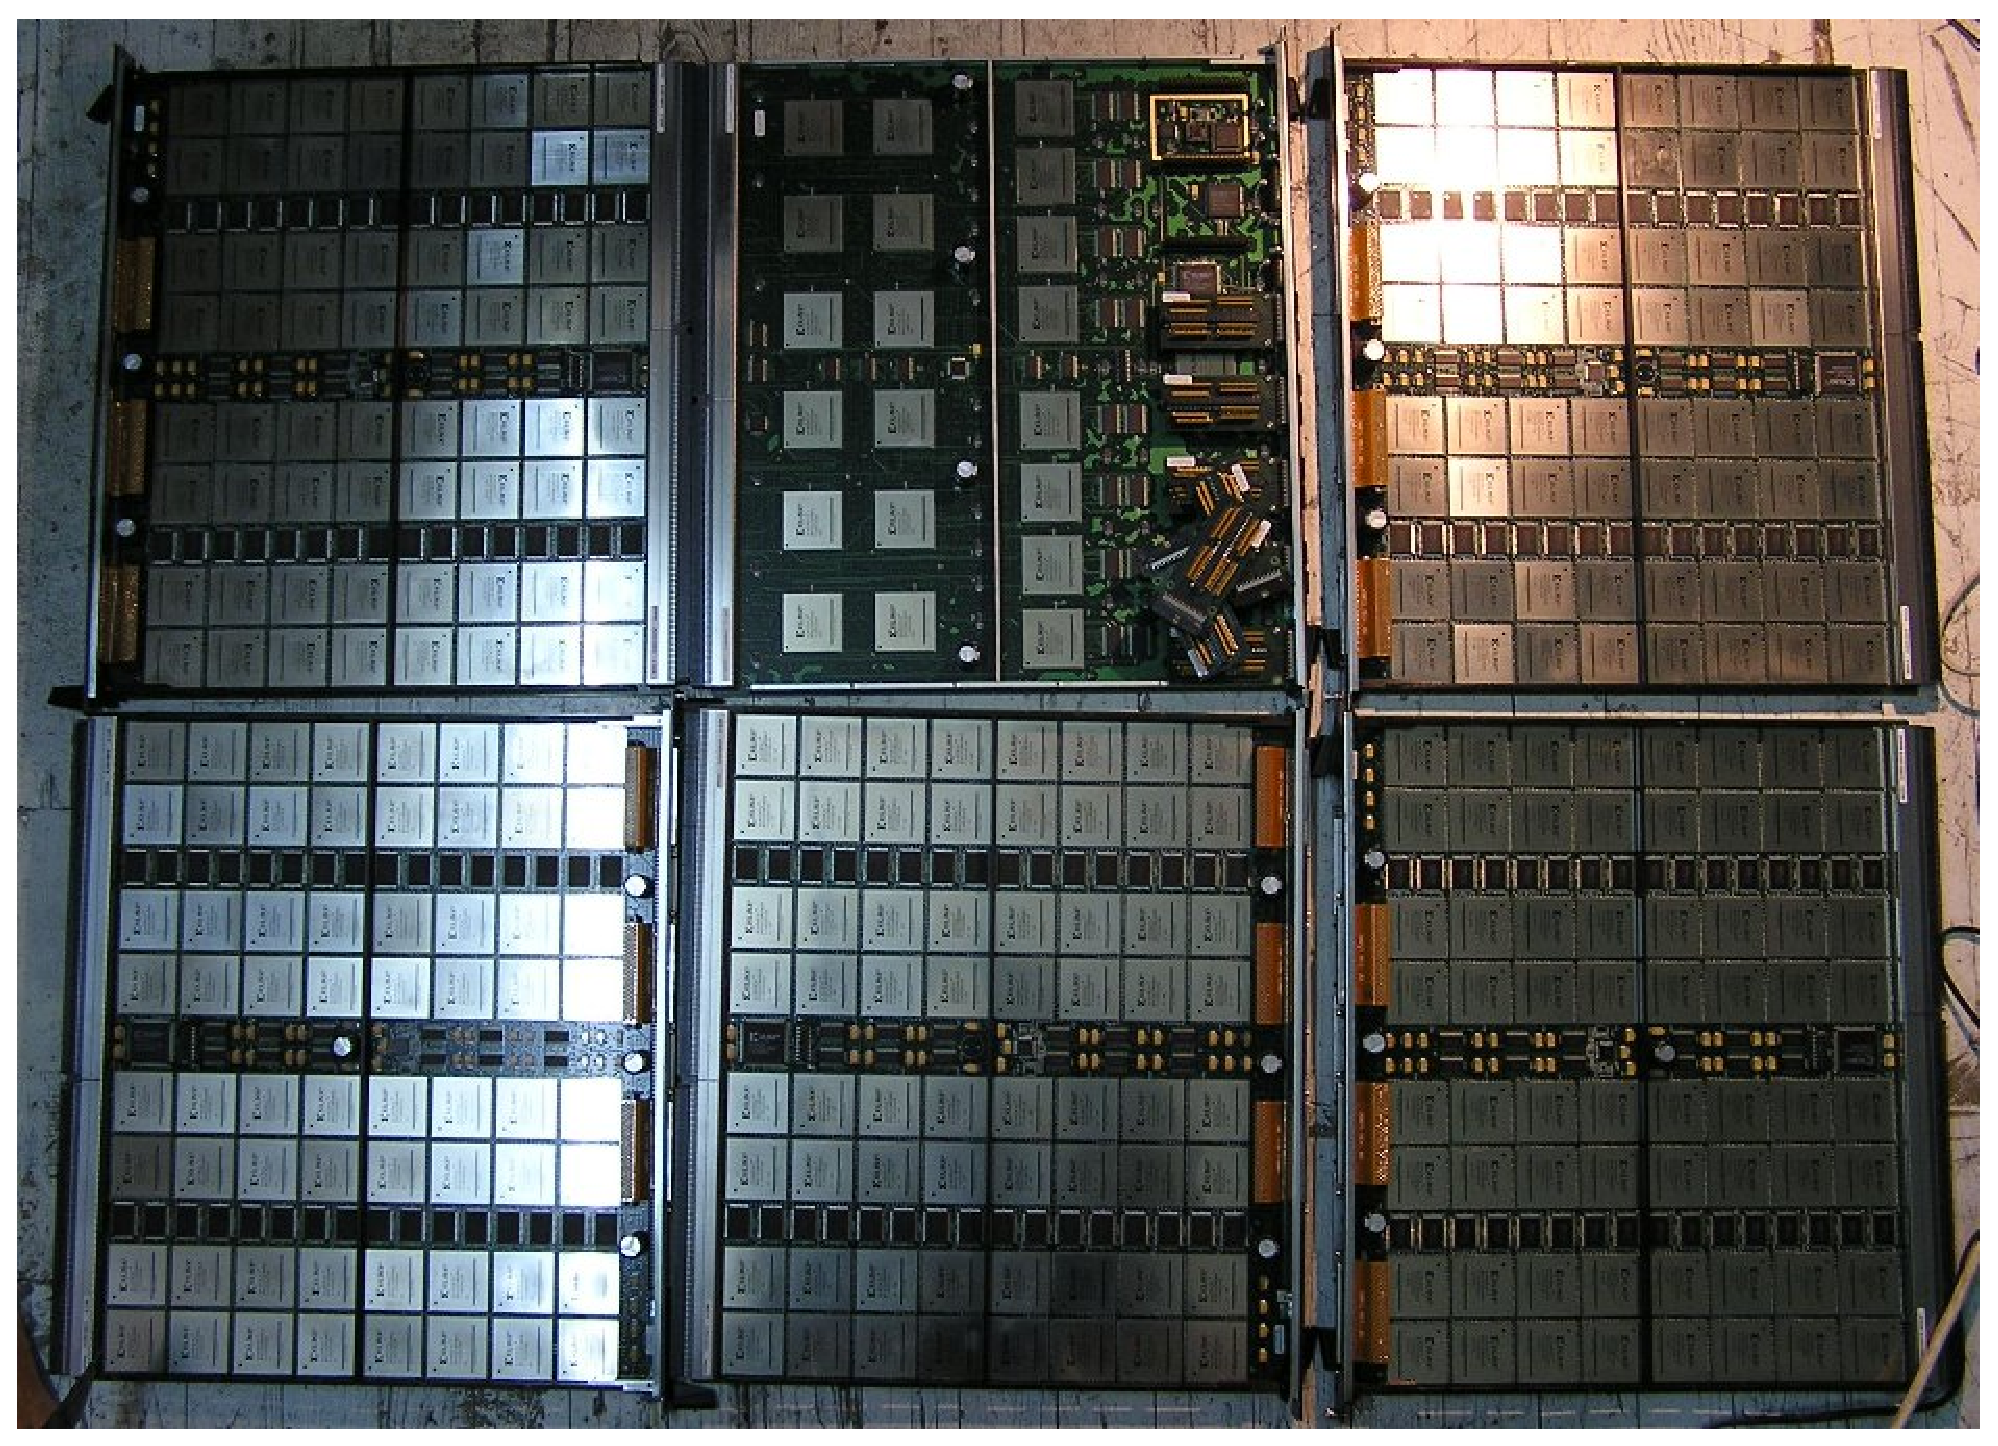
\includegraphics[height=95mm]{ikosboards.eps}
\caption{FPGA boards of the Ikos Pegasus ASIC emulator (ca. 1999).}
\label{fig:ikos}
\end{figure}

But the cost of FPGAs is falling (this was already the case between 1985 and 1994~\cite{fpgacost} and the trend has continued since then) and relatively fast and high-density devices are today becoming available to the general public. For an example of this falling cost (and increasing densities and speed), we will mention the Ikos Pegasus application specific integrated circuit (ASIC) emulator, whose insides are depicted in figure~\ref{fig:ikos}. The LatticeMico32 CPU core used in the system-on-chip described in this thesis occupies alone 60\% of the resources of one of the XC4036XL FPGAs of this device, and runs at 30MHz. The Ikos Pegasus was a state-of-the-art device a decade ago. It consumes up to 3 kilowatts of power, weights dozens of kilos and probably costed the equivalent of several millions of SEK. The same CPU core now occupies about 15\% of a modern FPGA costing less than 500 SEK, where it runs in excess of 100MHz.

\begin{figure}
\centering
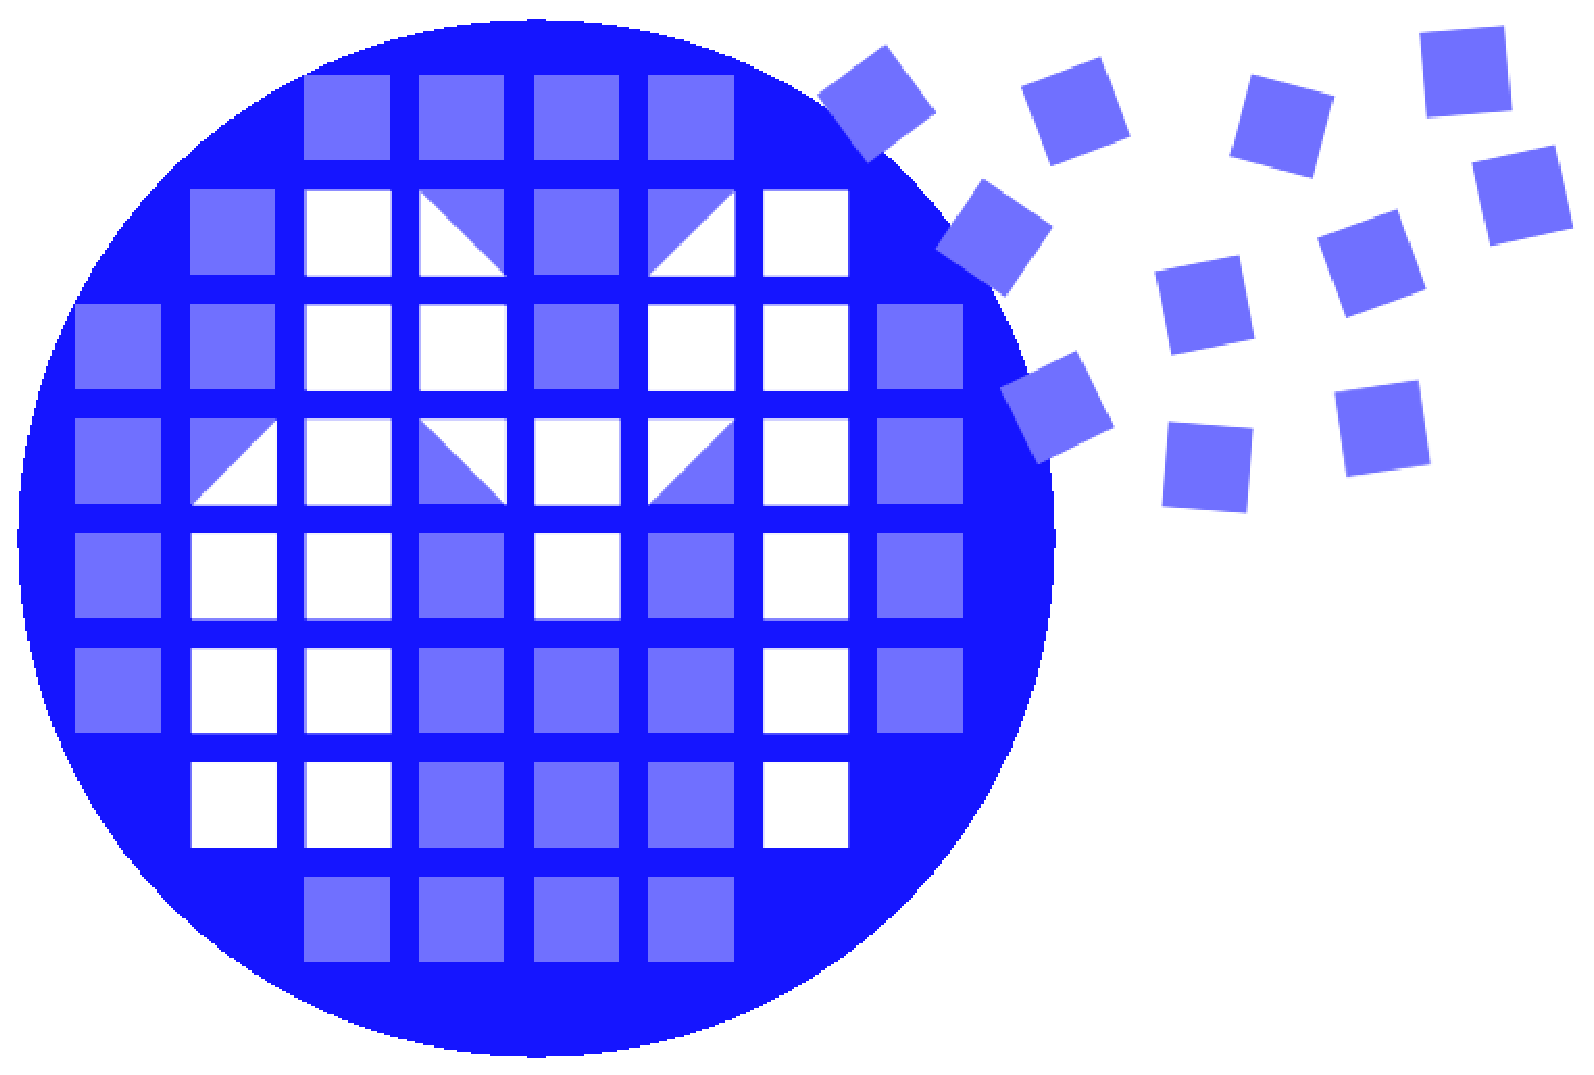
\includegraphics[height=55mm]{newlogo.eps}
\caption{Project logo.} \label{fig:projectlogo}
\end{figure}

This evolution makes it possible to implement complex high-performance system-on-chips (SoC) that can be modified and improved by anyone, thanks to the flexibility of the FPGA platform.

This master thesis introduces Milkymist\texttrademark \cite{milkymist}, a fast and resource-efficient FPGA-based system-on-chip designed for the application of rendering live video effects during performances such as concerts, clubs or contemporary art installations. Such effects are already popularized by artists known as ``video jockeys'', or ``VJs''. VJing is commonly done with a PC and computer software such as GrandVJ~\cite{grandvj} or Resolume~\cite{resolume}. However, this approach has some drawbacks and using an embedded device instead would be interesting:
\begin{itemize}
\item A device of very small size and weight is possible, which is convenient in mobile or temporary setups.
\item Boot and set-up time (launching the software) can be greatly reduced (to a few seconds).
\item Many interfaces for interactive performances (MIDI, DMX, video input, low-level digital I/O for user sensors) can be integrated. By comparison, the equivalent PC-based solution would be expensive and bulky.
\end{itemize}

Besides the fact that this is an interesting, creative and popular application, it is also demanding in terms of computational power and memory performance. Such a project would also be a proof that high performance open source system-on-chip design is possible in practice; with a view to help, foster and catalyze similar ``open hardware'' initiatives. As the Milkymist system-on-chip is entirely made of synthesizable Verilog and, for the most part, released under the GNU General Public License (GPL), its code can be re-used by other open hardware projects.

Meeting the performance constraints while still using cheap and relatively small FPGAs is perhaps the most interesting and challenging technical point of this project, and it could not be done without substantial work in the field of computer architecture. This is what this master thesis covers.

\chapter{Background}
\section{Video synthesis}
\subsection{Overview}
MilkDrop~\cite{milkdrop} (figure~\ref{fig:milkdrop}) is a popular open source video synthesis framework that was originally made to develop visualization plugins for the Winamp audio player. People have since then ported MilkDrop to many different platforms~\cite{wpmilkdrop} and made it react to live events, such as captured audio and video~\cite{visikord} (figure~\ref{fig:visikord}) or movements of a Wiimote remote control~\cite{wiimodemd}.

The idea behind the Milkymist project is to implement an embedded video synthesis platform on a custom open source system-on-chip, that is based on the same rendering principle of MilkDrop but with more control interfaces and features. The device built around the system-on-chip should be stand-alone, which means that a graphical user interface for configuring the visual effects should be implemented (figure~\ref{fig:flickernoise}).

\begin{figure}[htp]
\centering
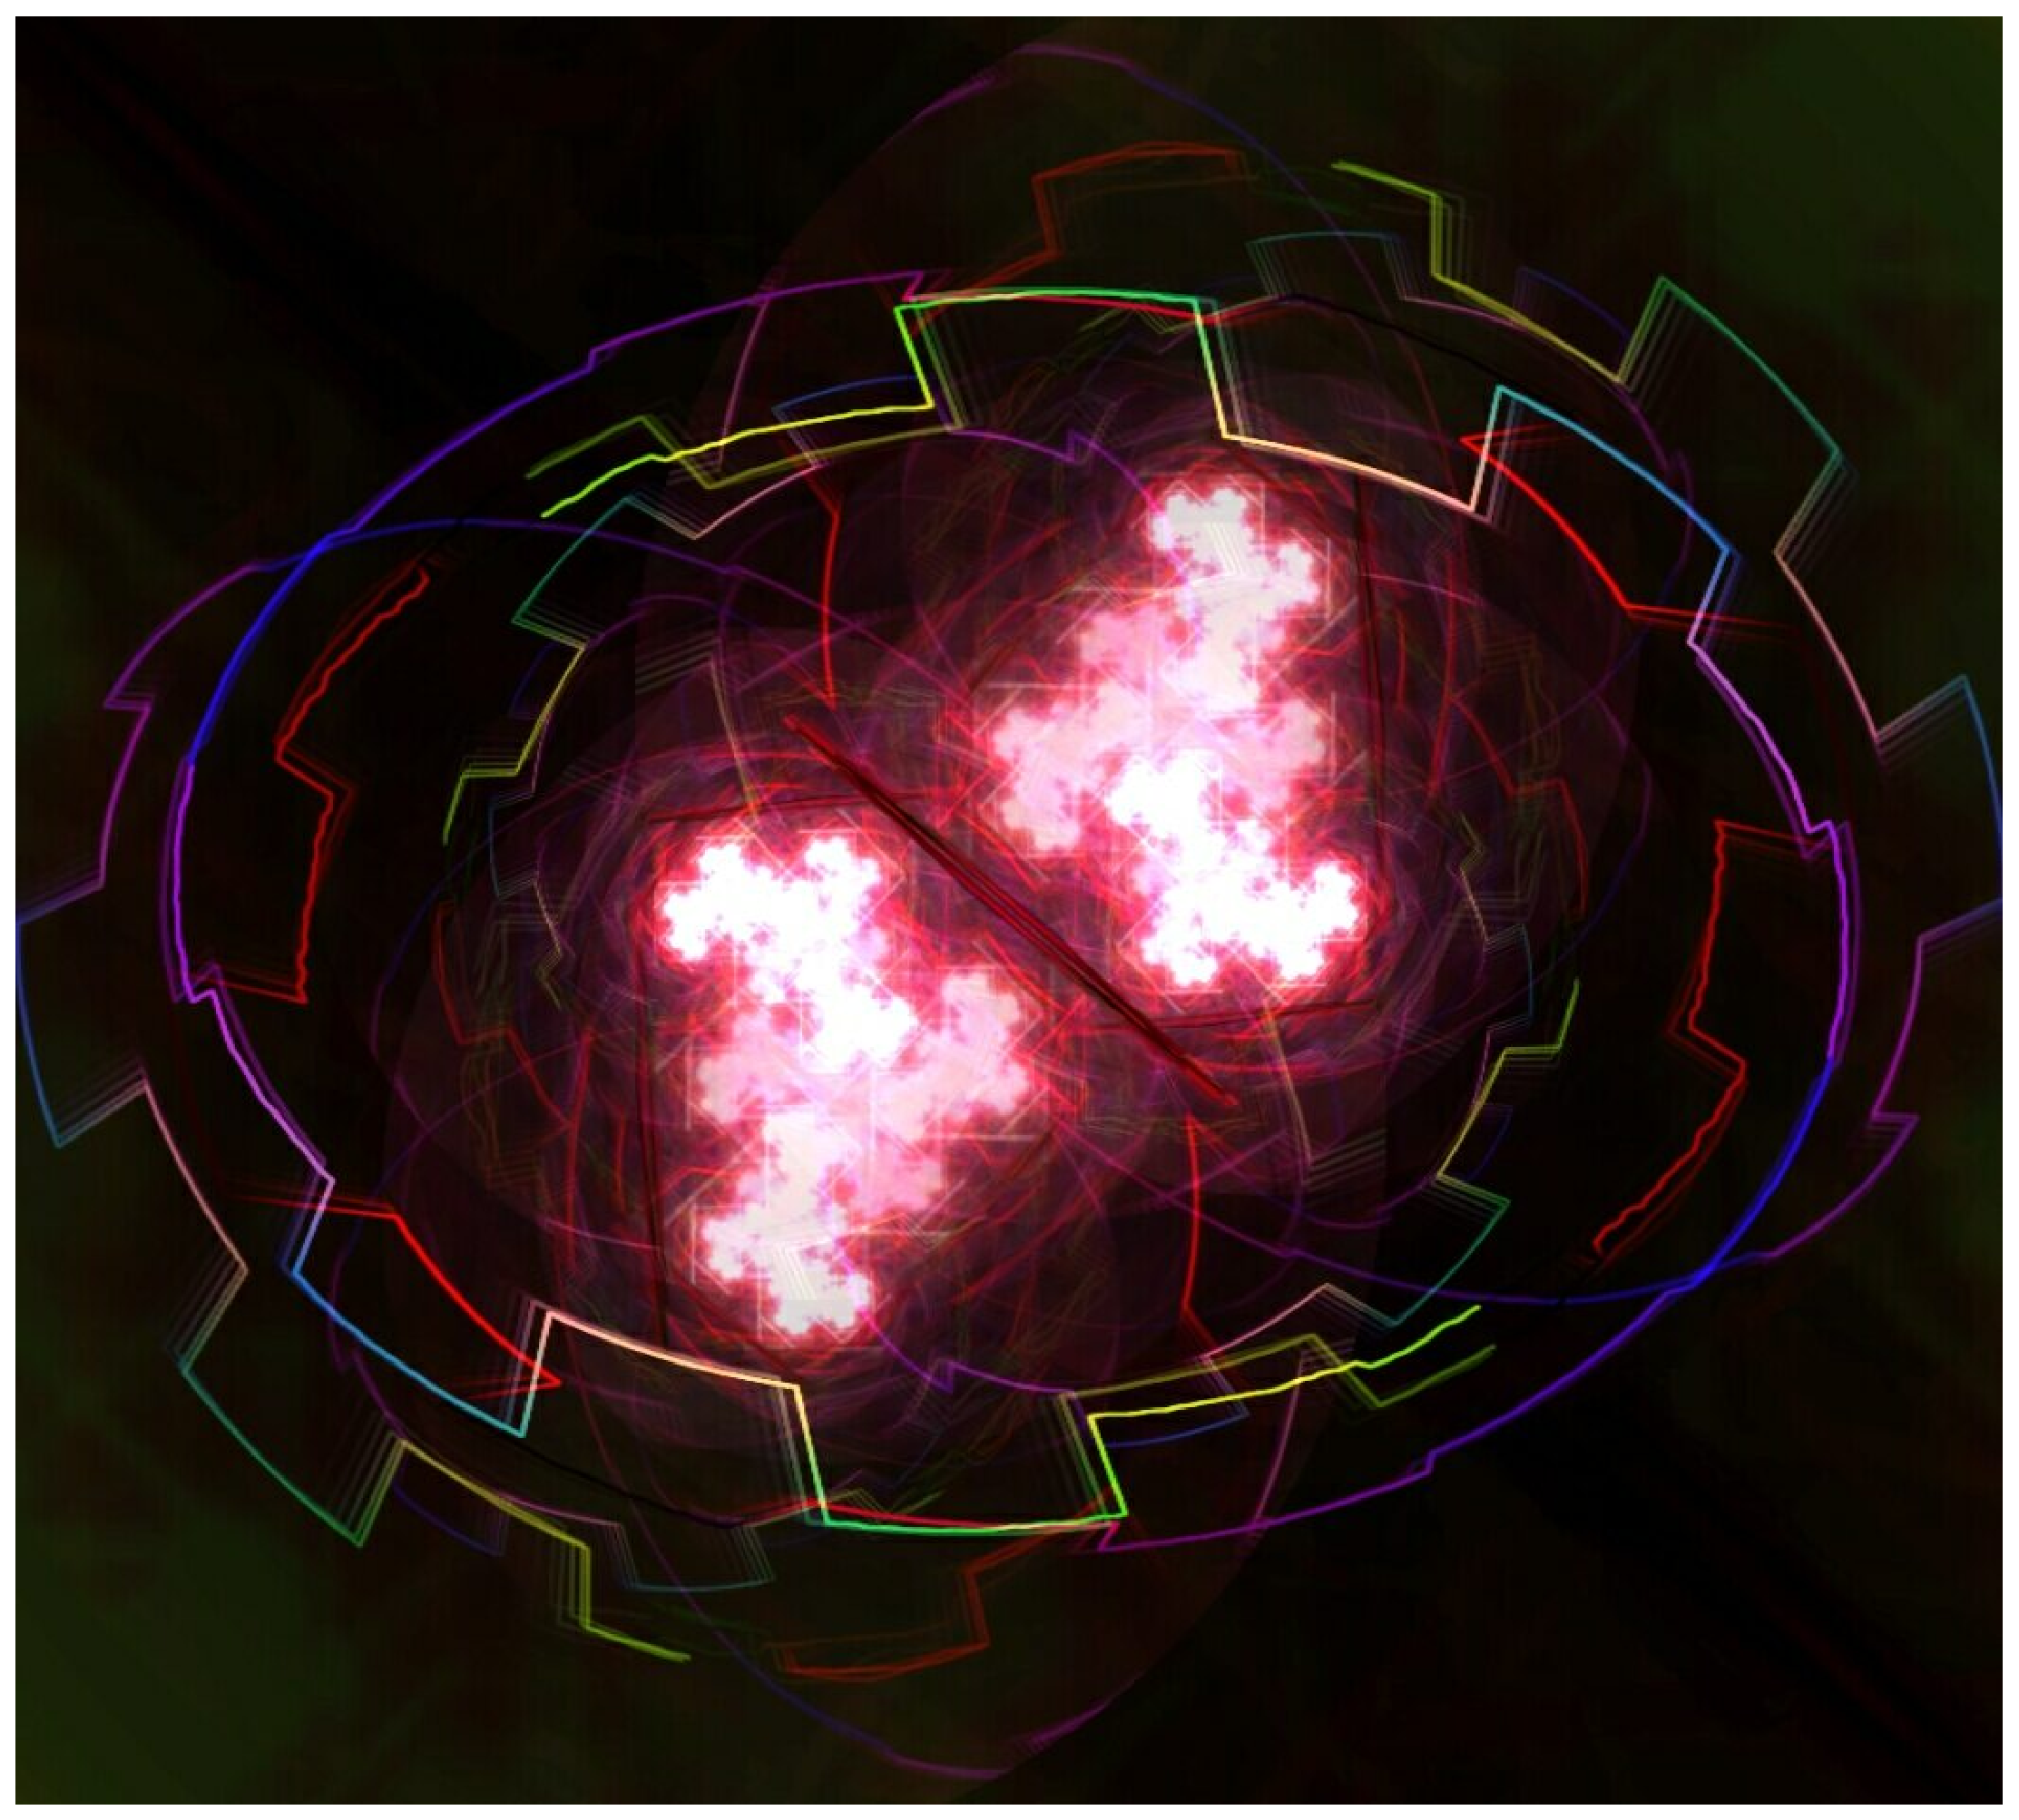
\includegraphics[height=65mm]{milkdrop2.eps}
\caption{Sample video frame from the MilkDrop visual synthesizer.}
\label{fig:milkdrop}
\end{figure}

\begin{figure}[htp]
\centering
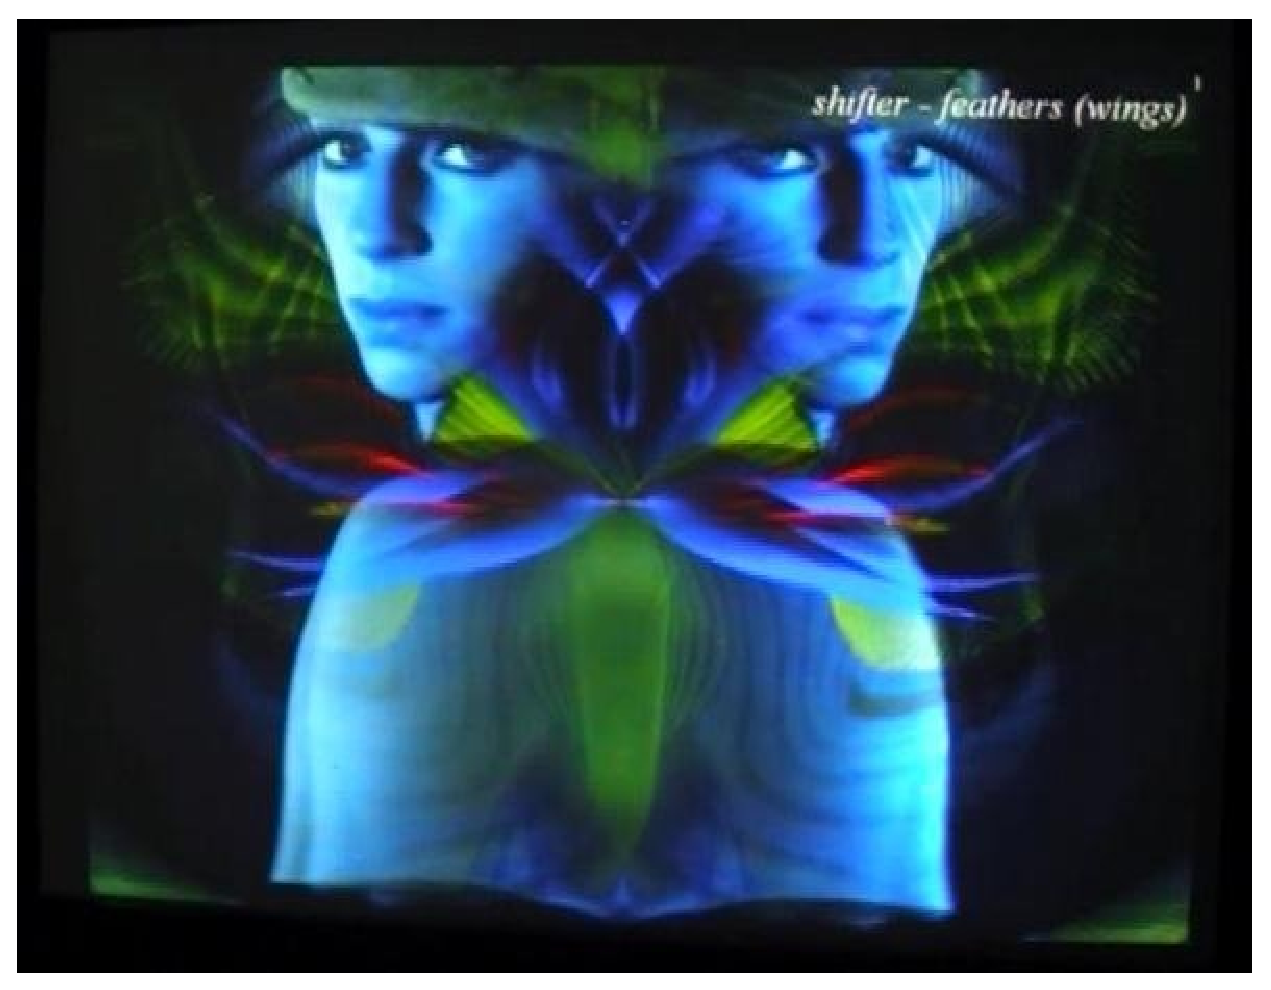
\includegraphics[height=60mm]{visikord.eps}
\caption{Sample video frame from Visikord, a program mixing live video into MilkDrop.}
\label{fig:visikord}
\end{figure}

\begin{figure}[htp]
\centering
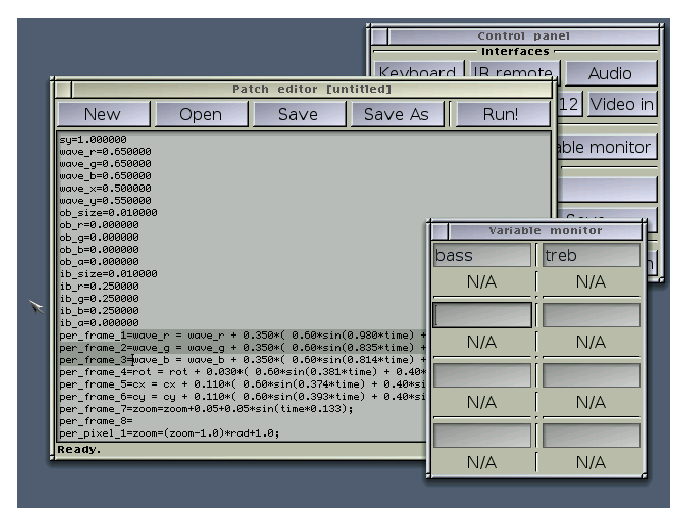
\includegraphics[height=85mm]{flickernoise.eps}
\caption{The embedded user interface (based on Genode FX~\cite{genodefx}) of Flickernoise, the Milkymist VJ application. The patch editor is shown, with per-frame and per-vertex equations.}
\label{fig:flickernoise}
\end{figure}

\subsection{Principle}
\label{subsec:mdprinciple}
\subsubsection{General mode of operation}
The MilkDrop-like renderer is the most compute and memory intensive process, from which stem most of the technical challenges. We will now get into more details about how the renderer works.

Rendering is based on a framebuffer on which the steps below are continuously repeated. This repetition is at the origin of many feedback or ``fractal'' effects.
\begin{itemize}
\item The current frame is distorted (zoomed, translated, warped, scaled, rotated...) by texture mapping. This step will be described with more detail in section~\ref{sec:tm}.
\item The frame is darkened (the colors are shifted to black).
\item A waveform of the currently played music is drawn. The wave can be drawn linearly (like an oscilloscope), in a circle, etc.
\item Borders around the screen are drawn. If the distortion zooms out, the borders will be pulled into the picture (some effects are based on this).
\item \textit{Motion vectors} are drawn. Motion vectors are simply a grid of dots, which can be used to generate effects by playing with the distortion.
\item The process repeats from the beginning.
\end{itemize}

These are the basic features of MilkDrop. There are more (custom waves, shapes,...) which are listed on the MilkDrop website~\cite{milkdrop}. Some other features (such as adding live video) will be added to the Milkymist renderer in the future.

This process is done on an internal framebuffer whose horizontal and vertical dimensions are a power of 2. This framebuffer is then scaled to the size of the screen in order to be displayed. This brings two features:
\begin{itemize}
\item The sizes being a power of 2 allows out-of-bounds texture coordinates to be wrapped (in order to repeat the texture) by simply performing a bitwise AND of the coordinate, instead of the full computation of a division remainder which is a much more expensive operation (even on the traditional GPUs MilkDrop was designed for).
\item It enables the implementation of the \textit{video echo} effect: after the internal framebuffer has been drawn to the screen at its nominal dimensions, a zoomed and semi-transparent copy of it can be overprinted.
\end{itemize}
It must be noted that this two-step process increases the computation time and the consumption of memory bandwidth.

All the steps of the rendering are heavily parametrizable by the user, using a coded format called a \textit{patch} or \textit{preset} which defines the aspect and the interaction forms of a particular visual effect. The listing of a sample patch is given by figure~\ref{fig:samplepatch} and the meaning of the language is explained below.

\begin{figure}
\centering
\begin{boxedminipage}{13cm}
\begin{verbatim}
fDecay=0.980000
nWaveMode=2
bTexWrap=1
bMotionVectorsOn=0
zoom=1.046000
rot=0.020000
cx=0.500000
cy=0.500000
warp=0.969000
sx=1.000000
sy=1.000000
wave_r=0.600000
wave_g=0.600000
wave_b=0.600000
wave_x=0.500000
wave_y=0.470000
per_frame_1=wave_r = wave_r + 0.400*( 0.60*sin(0.933*time)
  + 0.40*sin(1.045*time) );
per_frame_2=wave_g = wave_g + 0.400*( 0.60*sin(0.900*time)
  + 0.40*sin(0.956*time) );
per_frame_3=wave_b = wave_b + 0.400*( 0.60*sin(0.910*time)
  + 0.40*sin(0.920*time) );
per_frame_4=zoom = zoom + 0.010*( 0.60*sin(0.339*time)
  + 0.40*sin(0.276*time) );
per_frame_5=rot = rot + 0.050*( 0.60*sin(0.381*time)
  + 0.40*sin(0.579*time) );
per_frame_6=cx = cx + 0.030*( 0.60*sin(0.374*time)
  + 0.40*sin(0.294*time) );
per_frame_7=cy = cy + 0.030*( 0.60*sin(0.393*time)
  + 0.40*sin(0.223*time) );
per_vertex_1=sx=sx-0.04*sin((y*2-1)*6+(x*2-1)*7+time*1.59);
per_vertex_2=sy=sy-0.04*sin((x*2-1)*8-(y*2-1)*5+time*1.43);
\end{verbatim}
\end{boxedminipage}
\caption{Excerpt from the MilkDrop preset ``Geiss -- Warp of Dali 1'' (with some simplifications).}
\label{fig:samplepatch}
\end{figure}

\subsubsection{Initial conditions}
The patch begins with a series of parameters which are used to initialize the renderer, and many of them are kept constant during the execution of the patch. For example:
\begin{itemize}
\item \verb!bMotionVectorsOn=0! turns off the drawing of the motion vectors.
\item \verb!nWaveMode=2! selects one of the many ways of drawing the audio waveform.
\item \verb!sx=1.000000! and \verb!sy=1.000000! set the X and Y scaling factors of the distortion to 1 (i.e. the frame is initially not scaled).
\item \verb!wave_r=0.600000!, \verb!wave_g=0.600000! and \verb!wave_b=0.600000! set the initial RGB color with which the wave is drawn (it is initially grey).
\end{itemize}

\subsubsection{Per-frame equations}
Using initial conditions only limits the interaction and evolution possibilities of the patch.

It is therefore possible to make the parameters evolve over time, thanks to the per-frame equations. As their name suggests, the per-frame equations are mathematical expressions that are evaluated at each frame.

The example patch (figure~\ref{fig:samplepatch}) shows some of them (the lines beginning with \verb!per_frame!). In this example, they change the wave color over time by modifying the \verb!wave_r!, \verb!wave_g! and \verb!wave_b! values in sinusoidal patterns, as well as the zoom, rotation (\verb!rot!) and center of rotation (\verb!cx! and \verb!cy!).

Per-frame equations can make the patch react to sound, for example through the \verb!bass!, \verb!mid! and \verb!treb! variables that indicate the intensity of the sound in three frequency bands. One of the ideas in Milkymist is to add other variables that can be controlled by the DMX512 and MIDI protocols, enabling the use of a whole range of devices commonly found among musicians (electronic instruments, faders, stage light consoles, joysticks,...) to control the visual effects.

\subsubsection{Per-vertex equations}
Per-vertex equations are used to fine-tune the distortion applied to the picture.

Indeed, as explained further in section~\ref{sec:tm}, the distortion works by using a mesh of control points (vertices) that can be moved to transform the image in many different ways (effects such as zooming, scaling and rotating are implemented by moving the vertices).

Per-vertex equations are thus evaluated at each vertex (whose position can be retrieved through the \verb!x! and \verb!y! variables), and alter the position of that vertex. In the example patch (figure~\ref{fig:samplepatch}), the image is locally scaled horizontally and vertically by factors depending on the position of the vertex and on the time, resulting in a twisted visual effect.

As discussed in chapter~\ref{ch:tmu}, the floating point computations for each vertex are intensive and required the use of a dedicated coprocessor.

\section{Open source SoC platforms}
There is an existing effort to build open source system-on-chips. It is interesting to review these projects in order to look forward to building upon them --- possibly adding hardware accelerators or performing other modifications in order to improve performance.

There are many SoC designs available on the Internet, which are more or less mature. The system-on-chip projects listed here meet the following criteria:
\begin{itemize}
\item they have been shown to work on at least one FPGA board
\item they are released under an open source license
\item they comprise a synthesizable RISC CPU
\item the CPU is supported by a C and C++ compiler
\item they include a RS232 compatible UART (for a debug console)
\item they support interfacing to off-chip SDRAM memory
\end{itemize}

\subsubsection{OpenSPARC}
OpenSPARC~\cite{opensparc} is the well-known SPARC processor of Sun Microsystems which is now released under an open source license and included into a SoC FPGA project.

Implemented on a FPGA, this processor is extremely resource-intensive. A cut-down version of the CPU core only, called the ``Simply RISC S1'', occupies at least 37000 FPGA look-up tables (LUT) without the caches~\cite{simplyrisc}. This is about twice the logic capacity of the Virtex-4 XC4VLX25 FPGA.

As it turns out, the OpenSPARC architecture is a very complex design which implements a huge number of techniques which increase the software execution speed (instructions per clock cycle). While this is a wise choice for a software-centric processor implemented on a fully custom semiconductor chip, with a FPGA process it is more appealing to keep the software processor simple in order to save resources and make room for custom hardware accelerators, taking advantage of the FPGA flexibility.

\subsubsection{GRLIB}
GRLIB~\cite{grlib} is a very professional and standard-compliant library of SoC cores. The library features a comprehensive set of cores: AMBA AHB/APB bus control elements, the LEON3 SPARC processor, a 32-bit PC133 SDRAM controller, a 32-bit PCI bridge with DMA, a 10/100/1000 Mbit Ethernet MAC,  16/32/64-bit DDR SDRAM/DDR2 SDRAM controllers and more.

However, its drawbacks are:
\begin{itemize}
\item Code complexity. GRLIB is written in VHDL and makes intensive use of custom types, packages, generate statements, etc.
\item Cores are not self-contained. GRLIB defines many ``building blocks'' that are used everywhere else in the code, making it difficult to re-use code in another project which is not based on GRLIB.
\item Significant FPGA resource usage. A system comprising the LEON3 SPARC processor with a 2-way set-associative 16kB cache and no memory management unit (MMU), the DDR SDRAM controller, a RS232 serial port, and an Ethernet 10/100 MAC uses 13264 FPGA look-up tables (LUT). They map to 79\% of the Virtex-4 XC4VLX25 FPGA. We have carried out the test with the Xst synthesizer, Xilinx ISE 11.3, and GRLIB 1.0.21-b3957 (GPL release) using the default provided synthesis scripts. This undermines the possibility of adding hardware acceleration cores. In~\cite{softcorecomp}, a significant resource usage was also reported for an older version of LEON.
\item Relatively low clock frequency. With the same parameters as above, the maximum clock frequency is 84MHz.
\end{itemize}

Because of these reasons, GRLIB was not retained.

\subsubsection{ORPSoC (OpenRISC)}
ORPSoC is based on the OpenRISC~\cite{openrisc} processor core, which is the flagship product of OpenCores, a community of developers of open source system-on-chips. ORPSoC is essentially maintained by ORSoC AB.

ORPSoC notably features the OpenRISC OR1200 processor core, the Wishbone~\cite{wishbone} bus, comprehensive debugging facilities, a 16550-compatible RS232 UART, a 10/100Mbps Ethernet MAC and a SDRAM controller.

Unfortunately, ORPSoC is resource-inefficient and buggy. The OpenRISC implementation is not well optimized for synthesis. We carried out tests on the August 17, 2009 OpenRISC release. Still using the XC4VLX25 FPGA as target, synthesis with Xst and Xilinx ISE 11.4 yields an utilization of 5077 LUTs for the CPU core only (using the default FPGA configuration: no caches, no MMU, multiplier, and with the implementation of the RAMs using the RAMB16 elements of the FPGA selected), running at approximately 100MHz. A similar resource usage is reported in~\cite{softcorecomp}. The synthesis report shows asynchronous control signals where there should not be (such as on the output of the program counter), which can be an indication of poor quality of the design. Other IP cores comprising ORPSoC have similar issues (we tested the 16550 UART and the Ethernet MAC). Finally, the provided SDRAM controller only supports the low-bandwidth 16-bit single data rate option, has a high latency due to the extensive use of clock domain transfer FIFOs, does not support pipelined transfers and has a poorly written code.

OpenRISC and ORPSoC therefore do not seem to be a good platform for the performance-demanding and resource-constrained video synthesis application.

\subsubsection{LatticeMico32 System}
This product~\cite{mico32} from the FPGA vendor Lattice Semiconductor is comparable to Microblaze~\cite{microblaze} and Nios II~\cite{nios} from its competitors, respectively Xilinx and Altera.

Like its competing products, LatticeMico32 System features a broad library of light, fast and FPGA-optimized SoC cores.

One interesting move made by Lattice Semiconductor is that parts of the LatticeMico32 System are released under an open source license, and most notably the custom LatticeMico32 microprocessor core. LatticeMico32 System is also based upon the Wishbone~\cite{wishbone} bus, whose specification is free of charge and freely distributable.

While it is perhaps technically possible to build Milkymist on top of the LatticeMico32 System, there are licensing issues concerning most notably the DDR SDRAM controller which is proprietary.

However, the LatticeMico32 microprocessor core is interesting. Synthesized for the XC4VLX25 with the 2-way set-associative caches, the barrel shifter, the hardware divider and the hardware multiplier enabled, it occupies only about 2400 4-LUTs and runs at more than 100MHz.

This microprocessor core has been retained for use in Milkymist, as described in chapter~\ref{ch:sw}.

\subsubsection{Microblaze and Nios II}
Even though we are not interested in proprietary designs, we still give a brief overview of the resource usage of Microblaze and Nios II systems as a comparison.

\paragraph{Microblaze.} In~\cite{softcorecomp}, the Microblaze core is reported to use approximately 2400 LUTs, like LatticeMico32. TODO: frequency.

\paragraph{Nios II.} According to an Altera report~\cite{niosbench}, Nios II/f uses 1600 Cyclone II LEs. A LE is mainly comprised of a 4-LUT and a register, which is comparable to the Virtex-4 architecture on which LatticeMico32 was tested. Thus, it seems that the Nios II core would be approximately two thirds of the area of LatticeMico32.

Some differences can be noted between the LatticeMico32 configuration and the Nios II/f configuration used in the Altera report:
\begin{itemize}
\item Caches are direct-mapped and 512 bytes (each).
\item There is no multiplier.
\item Nios II/f uses a dynamic branch predictor, while LatticeMico32 uses a static branch predictor.
\item The report does not say if the optional hardware divider, multiplier and shifter (that were enabled in LatticeMico32) were selected.
\end{itemize}

The Nios II is also reported to run at 140 MHz with this configuration and UART, JTAG UART, SDR SDRAM controller and timer peripherals. This is very fast, but cannot be compared to the LatticeMico32 results on Virtex-4 for two reasons:
\begin{itemize}
\item Routing resources and logic delays for the two FPGA families are different.
\item It is possible that Altera hand-tuned the Nios II processor to their FPGA technology.
\end{itemize}

\section{DRAM technology}
DRAM is by far today's dominant memory technology, often being the only affordable solution when relatively large densities (typically more than a few megabytes) are required. Unfortunately, DRAMs are not straightforward devices and we need preliminary knowledge specific to this technology in order to understand the choices discussed in chapter~\ref{ch:memory}. Indeed, in order to reduce system costs, the intelligence has been moved away from the memory chips and into the memory controller~\cite{dramlowcost}, leaving the controller designer with the task of dealing with the low-level details of the DRAM technology.

We will therefore explain how the SDRAM (synchronous DRAM) technology works. These principles are the same for the original single data rate (SDR) SDRAM, and for the subsequent double data rate DDR, DDR2 and DDR3 memories. In all that follows, we suppose that the logic level 0 is represented by a voltage of 0 volts, and a logic level 1 is represented by a positive voltage H.

A DRAM memory bank (figure~\ref{fig:drambank}) is organized as a two dimensional array of cells. Each cell is comprised of a transistor connected to a capacitor. A cell stores one bit of information, indicated by the presence or not of a charge in the capacitor. The transistor acts as a switch that connects the capacitor to the \textit{bit line} (vertical lines) when the \textit{word line} (horizontal lines) its gate is connected to carries a high logic level.

A decoder translates the row address presented to the DRAM device and activates one of the word lines, according to the address.

Each bit line is connected to a \textit{sense amplifier}, which is a positive feedback device that, when switched on, turns any voltage X on the bit line between 0 and H into 0 (if $X < \frac{H}{2}$) or H (if $X > \frac{H}{2}$). The set of sense amplifiers is called the \textit{page buffer}.

\begin{figure}
\centering
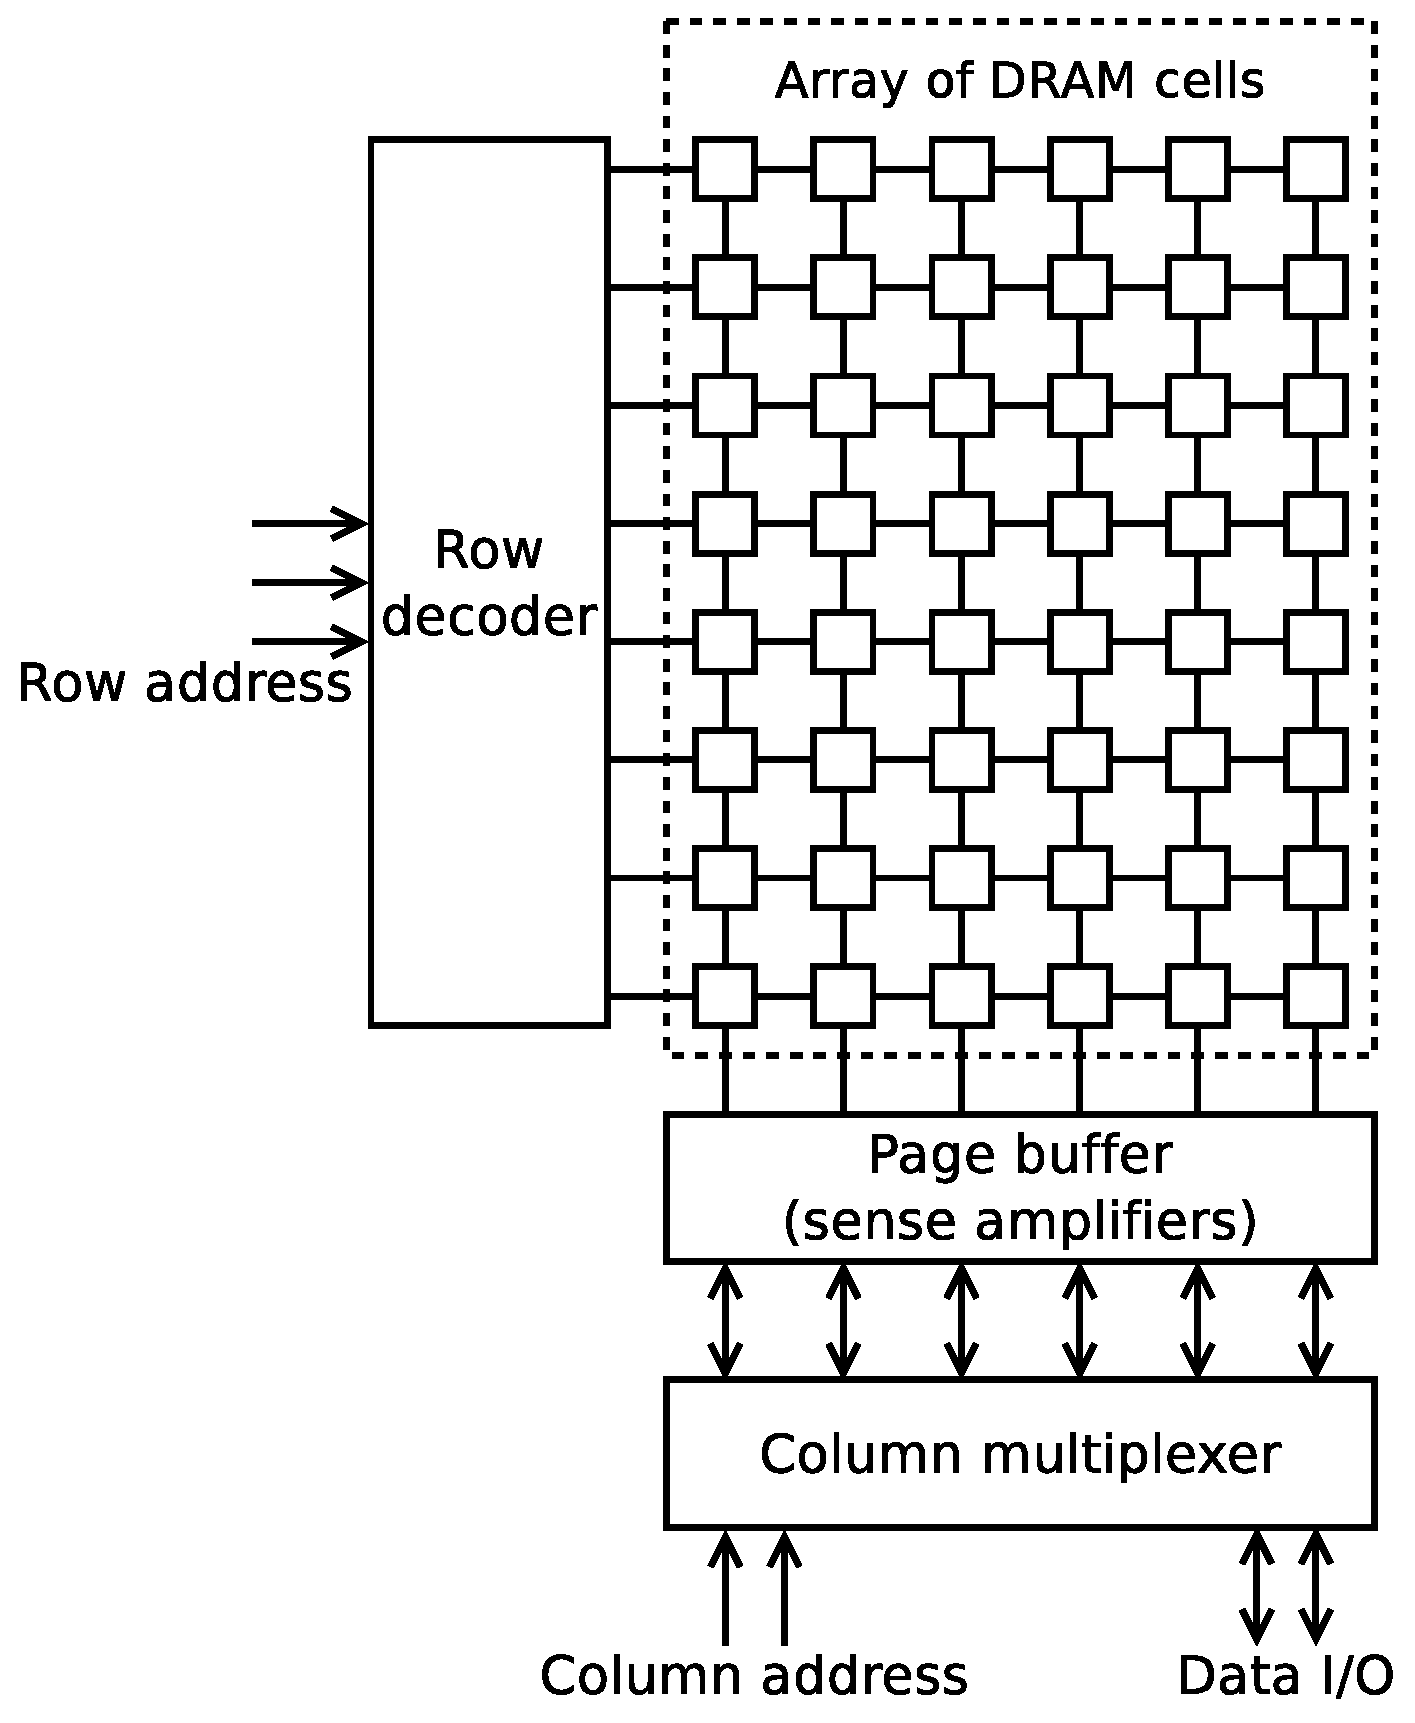
\includegraphics[height=100mm]{drambank.eps}
\caption{Block diagram of a DRAM memory bank.}
\label{fig:drambank}
\end{figure}

Accesses to a SDRAM bank are made as follows:
\begin{enumerate}
\item We assume the SDRAM is in the \textit{precharged} (idle) state. In this state, no word line is active, the sense amplifiers are turned off and all the bit lines are held at a voltage of $\frac{H}{2}$.
\item The SDRAM controller presents the row address and issues an ACTIVATE command. In response to this command, the SDRAM device enables the row decoder and one of the word lines is asserted. This has the effect of connecting all the capacitors of the DRAM cells in the row to their respective bit lines. A transfer of electric charge occurs between the ``parasitic'' capacitors of the word lines (which were charged at a voltage of $\frac{H}{2}$) and the DRAM cell capacitors, which were either discharged (at 0 volts) or charged at a voltage of H. This causes a small change $\epsilon$ in the potential of the bit line, which becomes $\frac{H}{2}-\epsilon$ or $\frac{H}{2}+\epsilon$ (depending on the charge initially stored in the DRAM cell capacitor). Then, the SDRAM device turns on all the sense amplifiers of the bank. On each bit line, the positive feedback takes over and amplifies the voltage difference $\epsilon$ until the level of the bit line reaches 0 or H. The ACTIVATE command is now completed and the row is said to be \textit{opened}. The DDR SDRAM chips used in the project (on the Xilinx ML401 board) take $20\unit{ns}$ to complete these operations.
\item Once a row has been opened, the controller can present the column address and issue READ and WRITE commands to transfer data. Reading is done by simply measuring the voltages on the bit lines, and writing can be achieved by forcing the bit lines to a particular level. There is a delay, called the CAS\footnote{CAS stands for Column Address Strobe, which is the name of the DRAM chip pin that the controller asserts at this stage.} latency, between a READ command being sent and the data being returned by the device. This delay is of $20\unit{ns}$ with the chips used in the project. However, read operations are pipelined, which means that a new READ command can be sent while the previous one is still transferring data. With proper scheduling, a full utilization of the available I/O bandwidth can be achieved.
\item Before accessing another row, the memory controller must disconnect the opened row from the bit lines and go back into the precharged state. It does so by issuing a PRECHARGE command to the device. The device takes some time to process the command (during which the bank cannot be accessed), which is $20\unit{ns}$ with the chips used in the project.
\end{enumerate}

From this principle of operation, it becomes apparent that a performance-oriented controller should try to make several transfers in the same row before opening another one, in order to reduce the time wasted to switching rows.

\subsection{Multiple banks}
SDRAM memory chips contain multiple DRAM banks internally, which share the I/O, command and address pins. Additional bank address pins select the bank to send commands to.

Having multiple banks brings two advantages:
\begin{itemize}
\item Being able to execute several commands simultaneously (assuming there is no resource conflict for the pins). For example, one bank can be activating one row while another bank is transferring data.
\item Having several rows open (one per bank), which can reduce the number of required row switches and thus improve performance.
\end{itemize}

The controller is responsible for managing the banks, and mapping absolute memory addresses to particular banks. Appropriate bank mapping can improve performance~\cite{pagemode}.

Standard DDR SDRAM chips come with four internal banks.

\subsection{Refreshing}
Because the DRAM capacitors are not perfect, they gradually lose their charge over time, which results in data corruption.

The solution is to periodically recharge the capacitors, which is done by opening the rows one by one. SDRAM chips provide an AUTO REFRESH command which opens and closes one row in all banks (and increments an internal counter so that the next AUTO REFRESH command will target another row), but it is the responsibility of the controller to issue it. Furthermore, the controller must precharge all banks before a refresh.

With the memory chips used in the project, a refresh must be made every $7.8\unit{\mu s}$ and takes in the worst case $20+80+4 \cdot 20=180\unit{ns}$ (precharge time\footnote{All banks can be precharged at the same time with a single command.} + refresh time + activation time for each bank), so it has a small impact on the memory bandwidth (about 2\%).

\section{Texture mapping}
\label{sec:tm}
Texture mapping is a common computer graphics operation found in accelerated 3D APIs like OpenGL and DirectX. It is typically used to draw textured 3D polygons on the screen. It can also distort an image (see figure~\ref{fig:distorted} for an example), and MilkDrop uses it for this purpose.

\begin{figure}
\centering
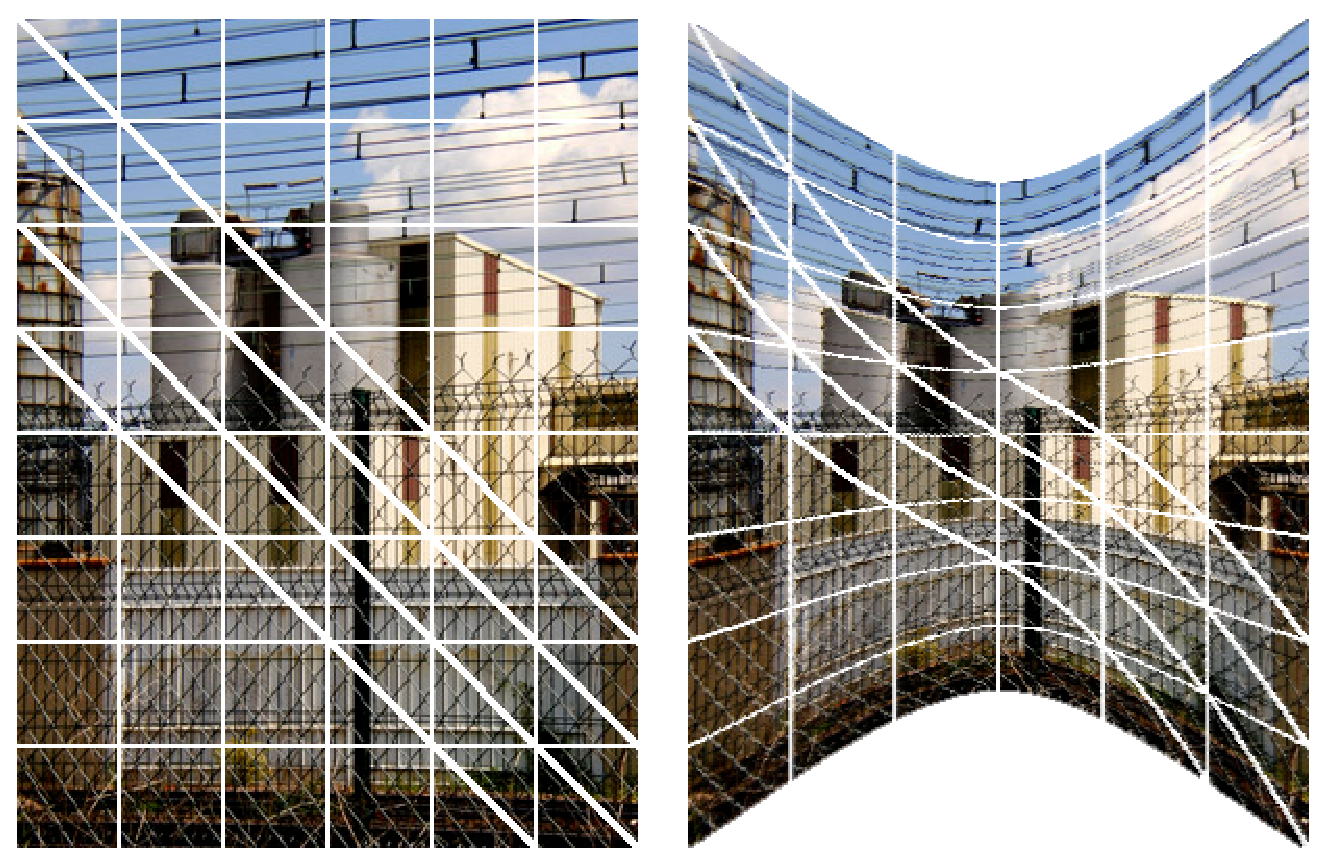
\includegraphics[height=70mm]{tesselsanofi.eps}
\caption{Example of distorted picture.}
\label{fig:distorted}
\end{figure}

With common GPUs, texture mapping is performed on triangles (and more complex polygons are broke down into a series of triangles). The inputs to the algorithm are the 2D (possibly projected from the original 3D coordinates) positions of the three vertices of the triangle to be filled, and the 2D texture coordinates for these three vertices.

The algorithm will then draw a textured triangle pixel by pixel, by interpolating linearly the texture coordinates of the vertices for each pixel and then copying the texture pixel (\textit{texel}) at these coordinates.

Image processing operations like zooming, rotating or scaling can be implemented with texture mapping, by simply changing the vertices' positions or the textures coordinates at each vertex.

More often than not, the results of the linear interpolation will not be integer, which means that the texture should be sampled between four adjacent pixels (figure~\ref{fig:bilinear}). In this case, for a better rendering, the four pixels should be read and their colors should be averaged (with different weights depending on the fractional parts). This process is called \textit{bilinear filtering} and is required to obtain a good rendering of MilkDrop presets (see figures \ref{fig:mdbilin} and \ref{fig:mdnearest}).

\begin{figure}
\centering
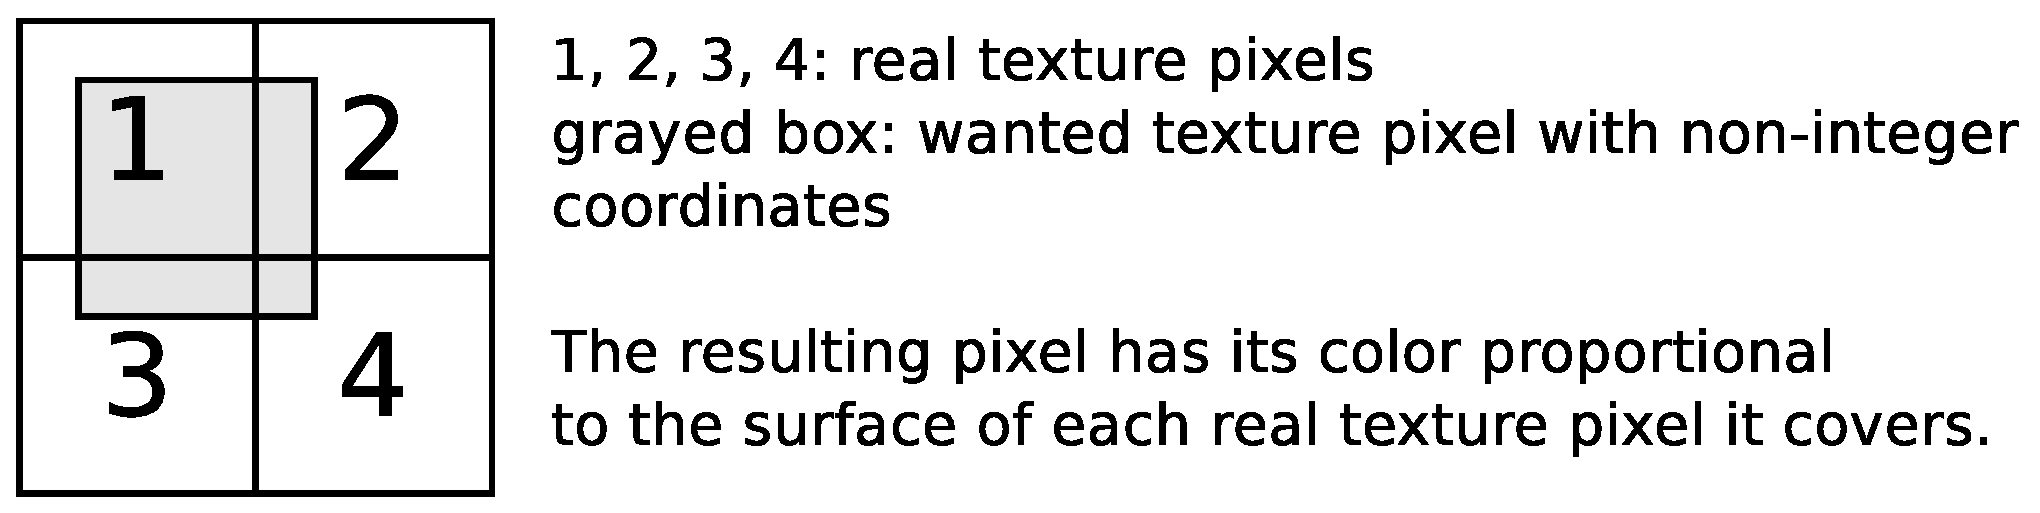
\includegraphics[height=30mm]{bilinear.eps}
\caption{Principle of bilinear texture filtering.}
\label{fig:bilinear}
\end{figure}

\begin{figure}
\centering
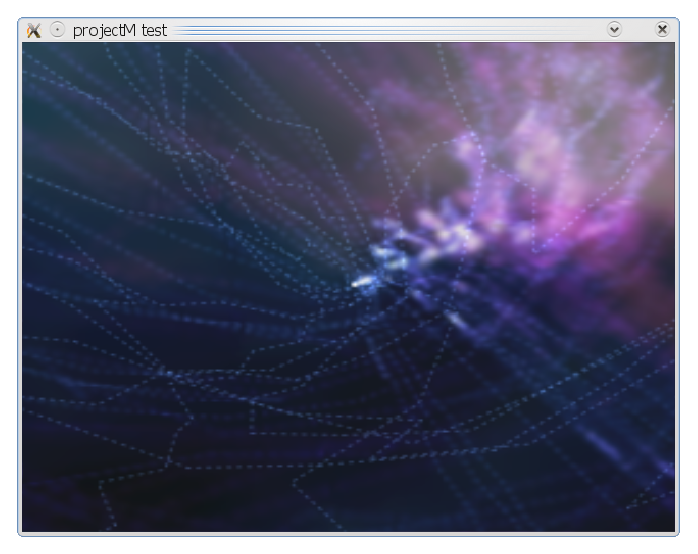
\includegraphics[height=70mm]{mdbilin.eps}
\caption{Rendering with bilinear filtering enabled.}
\label{fig:mdbilin}
\end{figure}

\begin{figure}
\centering
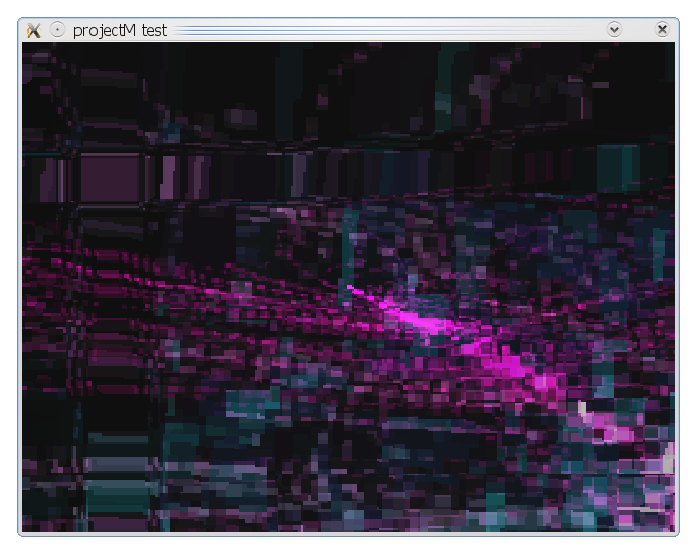
\includegraphics[height=70mm]{mdnearest.eps}
\caption{Rendering with bilinear filtering disabled (the nearest texel is used).}
\label{fig:mdnearest}
\end{figure}

In MilkDrop (and Milkymist), a special case of the texture mapping is used, as the only purpose is to distort a 2D image. The target surface is always a rectangle that covers the destination picture, on which the vertices are distributed evenly as a mesh which is always kept the same regardless of the applied distortion. The distortion is defined by altering the texture coordinates at each vertex.

Texture mapping, especially when bilinear filtering is desired, is a very compute intensive process, as explained in chapter \ref{ch:tmu}. A custom hardware accelerator has been developed, whose details are also covered in this chapter.

\section{Organization}
According to this background, we can derive the following project guidelines:

\begin{itemize}
\item develop a fast, resource-efficient and FPGA-optimized system-on-chip
\item develop an efficient memory subsystem
\item reuse a light-weight softcore CPU
\item partition carefully the tasks between hardware and software
\item develop custom hardware accelerators
\end{itemize}

The proposed solution is outlined in figure~\ref{fig:block}. Not all the blocks are ready at the time of this writing, nor all of them are within the scope of this Master's thesis, which focuses on computer architecture.

More specifically, the following components are not developed yet:
\begin{itemize}
\item microSD controller (the current prototype use a CF card through Xilinx SystemACE)
\item USB controller
\item Video input
\item IR receiver
\item MIDI controller
\item DMX512 controller
\end{itemize}

Hardware accelerators have been developed for the computation of vertices positions (PFPU) and for texture mapping (TMU), which have been found to be the most compute-intensive parts of the process. They are discussed in detail in chapters \ref{ch:pfpu} and \ref{ch:tmu}, respectively.

Graphics processing also requires a significant amount of memory bandwidth, which is discussed in chapter~\ref{ch:memory}.

Chapter~\ref{ch:intercon} describes the on-chip interconnect used to make the various blocks communicate with one another.

Finally, chapter~\ref{ch:sw} deals with the software execution environment and how the software is architected to obtain a good performances from the hardware.

\begin{figure}
\centering
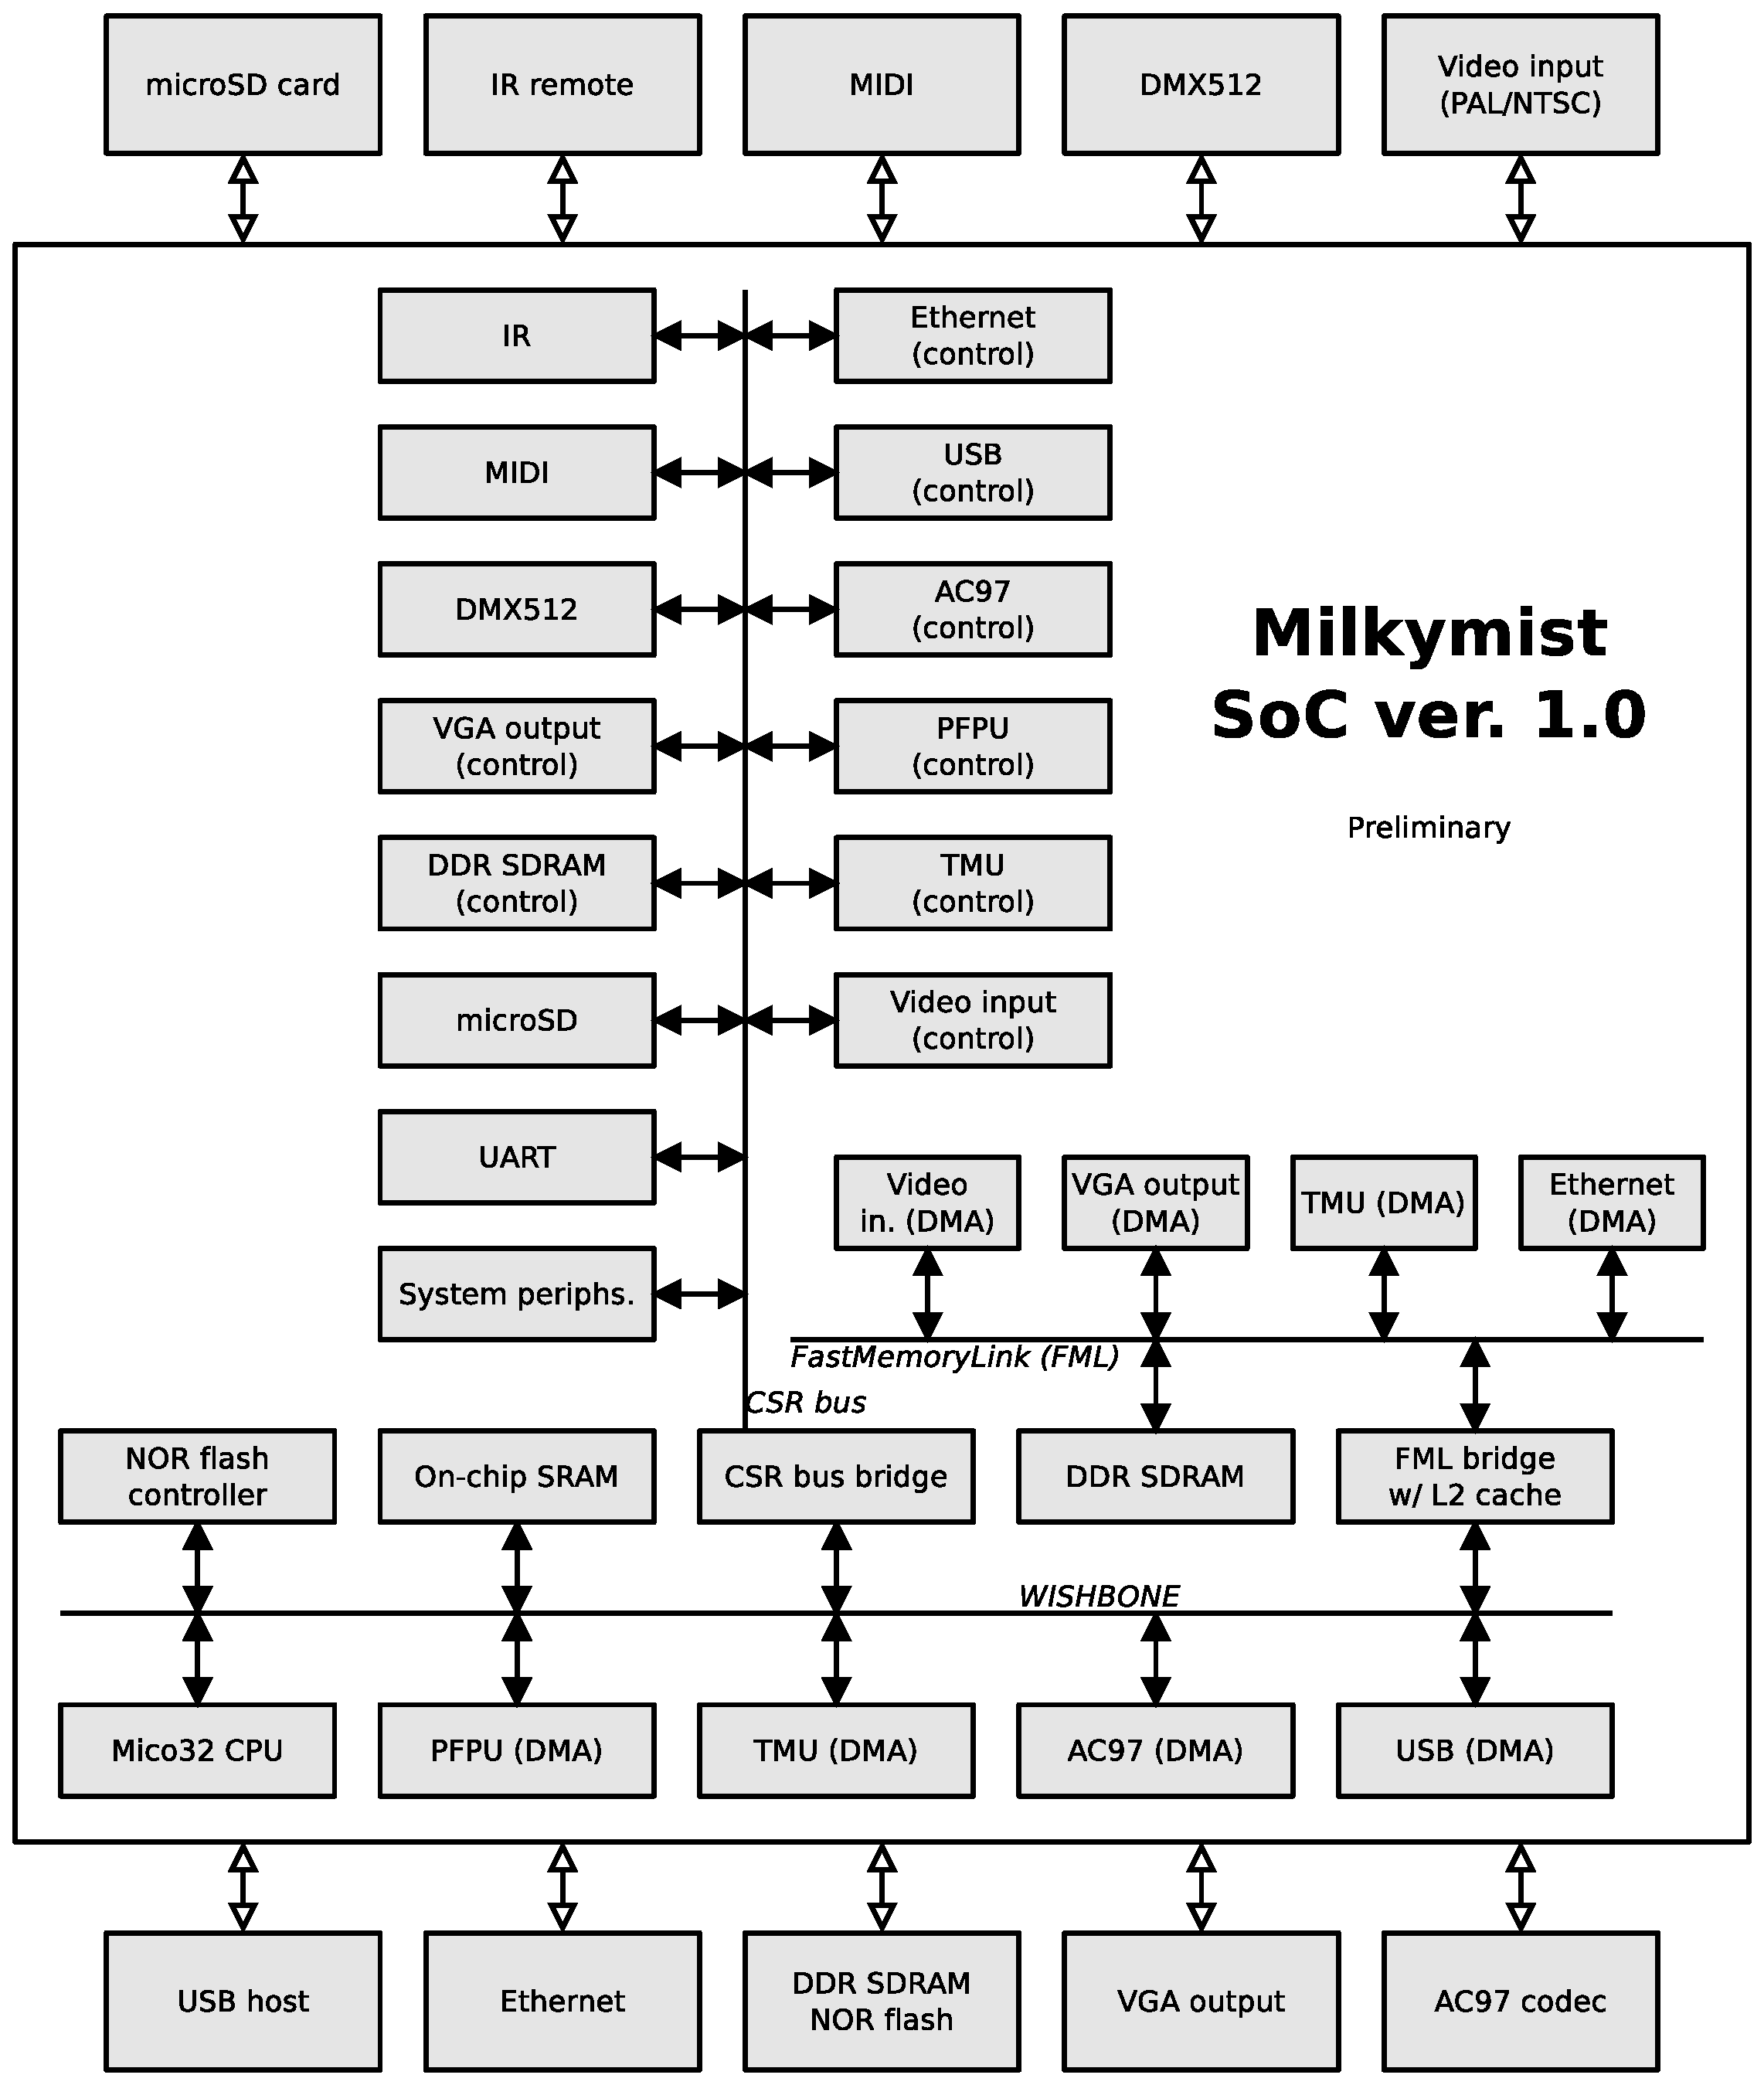
\includegraphics[height=170mm]{soc_architecture.eps}
\caption{SoC block diagram.}
\label{fig:block}
\end{figure}


\chapter{Memory subsystem}
\label{ch:memory}
\section{Attacking the memory wall}
\label{sec:memorywall}
A recurrent point in many modern computer systems is the memory performance problem. The term \textit{memory wall} was coined~\cite{memorywall} to refer to the growing disparity of performance between logic such as CPUs and off-chip memories. While microprocessor performance has been improving at a rate of 60 percent per year, the access time to DRAM has been improving at less than 10 percent per year~\cite{memvscpu}.

Memory performance is measured with two metrics:
\begin{itemize}
\item \textit{bandwidth}, which is the amount of data that the memory system can transfer during a given period of time.
\item \textit{latency}, which is the amount of time that the memory system spends between the issue of a memory read or write request and its completion.
\end{itemize}

A memory system can have both high bandwidth and latency. If the logic making the memory accesses is able to issue requests in a pipelined fashion, sending a new request without waiting for the previous one to complete, high latency will not have an impact on bandwidth.

Latency and bandwidth are however linked in practice. Decreasing the latency also increases the bandwidth in many cases, because latency blocks sequential processes and prevents them from utilizing the full available bandwidth.

High-end processors for servers and workstations have a good ability to cope with relatively high memory latency, because techniques such as out-of-order execution and hardware multi-threading enable the processor to issue new instructions even though one is blocking on a memory access.

Thus, most of today's SDRAM controllers do a lot to optimize bandwidth but have little focus on latency. Bandwidth-optimizing techniques include:
\begin{itemize}
\item reordering memory transactions to maximize the page mode hit rate.
\item grouping reads and writes together to reduce write recovery times. Along with the above technique, this has a detrimental impact on latency because of the delays incurred by the additional logic in the address datapath.
\item running the system and the SDRAM in asynchronous clock domains in order to be able to run the SDRAM at its maximum allowable clock frequency. This requires the use of synchronizers or FIFOs, which have a high latency.
\item configuring the SDRAM at high CAS latencies in order to increase its maximum allowable clock frequency. This trend is best illustrated by the advent of DDR2 and DDR3 memories whose key innovation is to run their internal DRAM core at a submultiple of the I/O frequency with a wide data bus which is then serialized on the I/O pins. Since the internal DRAM core has a latency comparable to that of the earlier SDR and DDR technologies, the number of CAS latency cycles relative to the I/O clock is also multiplied.
\end{itemize}

An extreme example of these memory controller bandwidth optimizations is the MemMax\textregistered ~DRAM scheduler~\cite{memmax}. This unit sits on top of an already existing memory controller (which already has its own latency), adding seven stages of complex and high-latency pipelining that produces a good - but compute-intensive - DRAM schedule. The actual efficiency of this system has been questioned~\cite{dramqos} because of that significant increase in latency.

\section{Another approach}
The out-of-order execution and hardware multithreading processor optimizations discussed above that cope with high memory latency are complex and impractical in the context of small and cheap embedded systems, especially those targetted at FPGA implementations. For example, FPGA implementations of the OpenSPARC~\cite{opensparc} processor, which employs such optimizations, typically require an expensive high-end Xilinx XUPV5 board whose Virtex-5 FPGA alone costs roughly 13000 SEK.

Milkymist therefore uses simple in-order execution schemes in its CPU and in its accelerators, and strives to improve performance by focusing on reducing the memory latency.

The memory system features that improve latency (but also bandwidth) are discussed below.

\section{Memory system features}
\subsection{Single SDRAM and system clock domain}
The typical operating frequency of early SDR and DDR SDRAM (technologies that are prior to DDR2 and do not have a clock divider for the internal DRAM core) is close to the 100MHz frequency at which the FPGA is able to meet timing for the complete SoC. Thus, it was decided to run the DRAM and the system synchronously in order to remove the need for any clock domain transfer logic and reduce latency. The SDRAM I/O registers are clocked by the system clock, and timing of the SDRAM interface is met through the use of calibrated on-chip delay elements and delay-locked-loops (DLLs) to generate the off-chip SDRAM clock and the data strobes.

\subsection{Page mode control algorithm}
The Milkymist memory controller takes the so-called \textit{page mode gamble}: after an access, the DRAM row is left open in the hope that the next transaction to the memory bank will occur within the same row. If the memory controller is right, the read or write command can be immediately registered into the SDRAM, and only the CAS or write latency is incurred. If the memory controller is wrong, it must first precharge the DRAM bank and open the correct row, causing extra delays.

Thus, if the memory controller is often wrong, taking the page mode gamble will actually impact performance negatively. However, a study has shown~\cite{pagemode} that, with typical memory timings, the point at which the gamble pays off is for a page hit probability of 0.375 only, attainable with many practical memory access patterns.

Page hit probability is improved by the ability of the Milkymist memory controller to track open rows independently in each of the four memory banks that commercial SDRAM chips are equipped with.

This optimization positively affects both latency and bandwidth.

\subsection{Burst accesses}
\label{subsec:fmlburst}
All memory accesses are made using bursts, i.e. when an access for a word is made, the following words are also read or written. Burst mode is a feature of the SDRAM chips: only one read of write command is sent to them, and several words are transferred on subsequent clock cycles.

Using bursts frees the bus and DRAM control signals while other words are transferred, allowing the issue of new commands overlapping the data phase of the previous transaction.

Burst access is a form of prefetching that improves latency. It is only efficient when the prefetched data can be used by the requesting bus master. In the Milkymist system-on-chip, this is often the case:
\begin{itemize}
\item The CPU core has caches which access memory by complete cache lines. Thus, if the cache line length is a multiple of the burst length, the bursts can be easily fully memorized.
\item The video framebuffer repeatedly reads the same block of data in a sequential manner, and can easily make full use of the prefetched data assuming that is has sufficient on-chip buffer space.
\item The texture mapping unit also has a cache and a write buffer which work well with burst accesses. This will be discussed in Chapter~\ref{ch:tmu}.
\end{itemize}

\subsection{Burst reordering}
\label{subsec:fmlborder}
This feature enables the use of the critical-word-first scheme in caches, reducing the overall memory latency.

When a request is issued at an address which is not a multiple of the burst length, the order of the words in the burst is changed so that the first word that comes out is the very word that is at the requested memory address. The prefetch address is then incremented and wraps to stay within the same burst.

For example, assuming a burst length of 4:
\begin{itemize}
\item a request at address 0 fetches words 0, 1, 2 and 3 (in this order)
\item a request at address 2 fetches words 2, 3, 0 and 1 (in this order)
\end{itemize}

\subsection{Pipelining}
\label{subsec:fmlpipe}
The memory bus of Milkymist~\cite{fml} is pipelined. During the transfer of the prefetched (burst) data, a new request can be issued. This is illustrated for a read request by the table below:

\begin{tabular}{|c|c|c|c|c|c|c|c|}
\hline
\textbf{Address} & A1 & A1 & A1 & A2 & A2 & A2 & A2 \\
\hline
\textbf{Data} & -- & -- & M(A1) & M(A1+1) & M(A1+2) & M(A1+3) & M(A2) \\
\hline
\end{tabular}\\

\begin{tabular}{|c|c|c|c|}
\hline
\textbf{Address (cont.)} & -- & -- & --\\
\hline
\textbf{Data (cont.)} & M(A2+1) & M(A2+2) & M(A2+3) \\
\hline
\end{tabular}

Together with burst access, this helps acheiving high performance: the memory controller can hide DRAM latencies and row switch delays by issuing the requests to the DRAM in advance, while the previous transaction is still transferring data.

\section{Practical implementation}
\label{sec:memimpl}
The Milkymist SoC uses 32-bit DDR SDRAM, configured to its maximum burst length of 8. Since the DDR SDRAM transfers two words per clock cycles (one on each edge), this is turned by the I/O registers into bursts of four 64-bit words synchronous to the system clock.

\begin{table}
\centering
\begin{tabularx}{13cm}{|X|l|}
\hline
\textbf{Task} & \textbf{Required bandwidth} \\
\hline
VGA framebuffer, 1024x768, 75Hz, 16bpp & 950Mbps \\
\hline
Distortion: texture mapping, 512x512 to 512x512, 30fps, 16bpp & 250Mbps \\
\hline
Live video: texture mapping, 720x576 to 512x512 with transparency, 30fps, 16bpp & 300Mbps \\
\hline
Scaling: texture mapping, 512x512 to 1024x768, 30fps, 16bpp & 500Mbps \\
\hline
Video echo: texture mapping, 512x512 to 1024x768 with transparency, 30fps, 16bpp & 900Mbps \\
\hline
NTSC input, 720x576, 30fps, 16bpp & 200Mbps \\
\hline
Software and misc. & 200Mbps \\
\hline
\textbf{Total} & \textbf{3.3Gbps} \\
\hline
\end{tabularx}
\caption{Estimate of the memory bandwidth consumption.}\label{tab:membw}
\end{table}

The memory is run at 100MHz, yielding a peak theoretical bandwidth of 6.4Gbps, which is more than enough for the intended video synthesis application (table~\ref{tab:membw}). This bandwidth is however never attained: events such as switching DRAM rows which takes significant time and, to a lesser extent, DRAM refreshes introduce dead times on the data bus. We will see in section~\ref{sec:memperf} that such an oversizing of the off-chip memory is needed if we want to keep the memory system simple.

\begin{figure}[H]
\centering
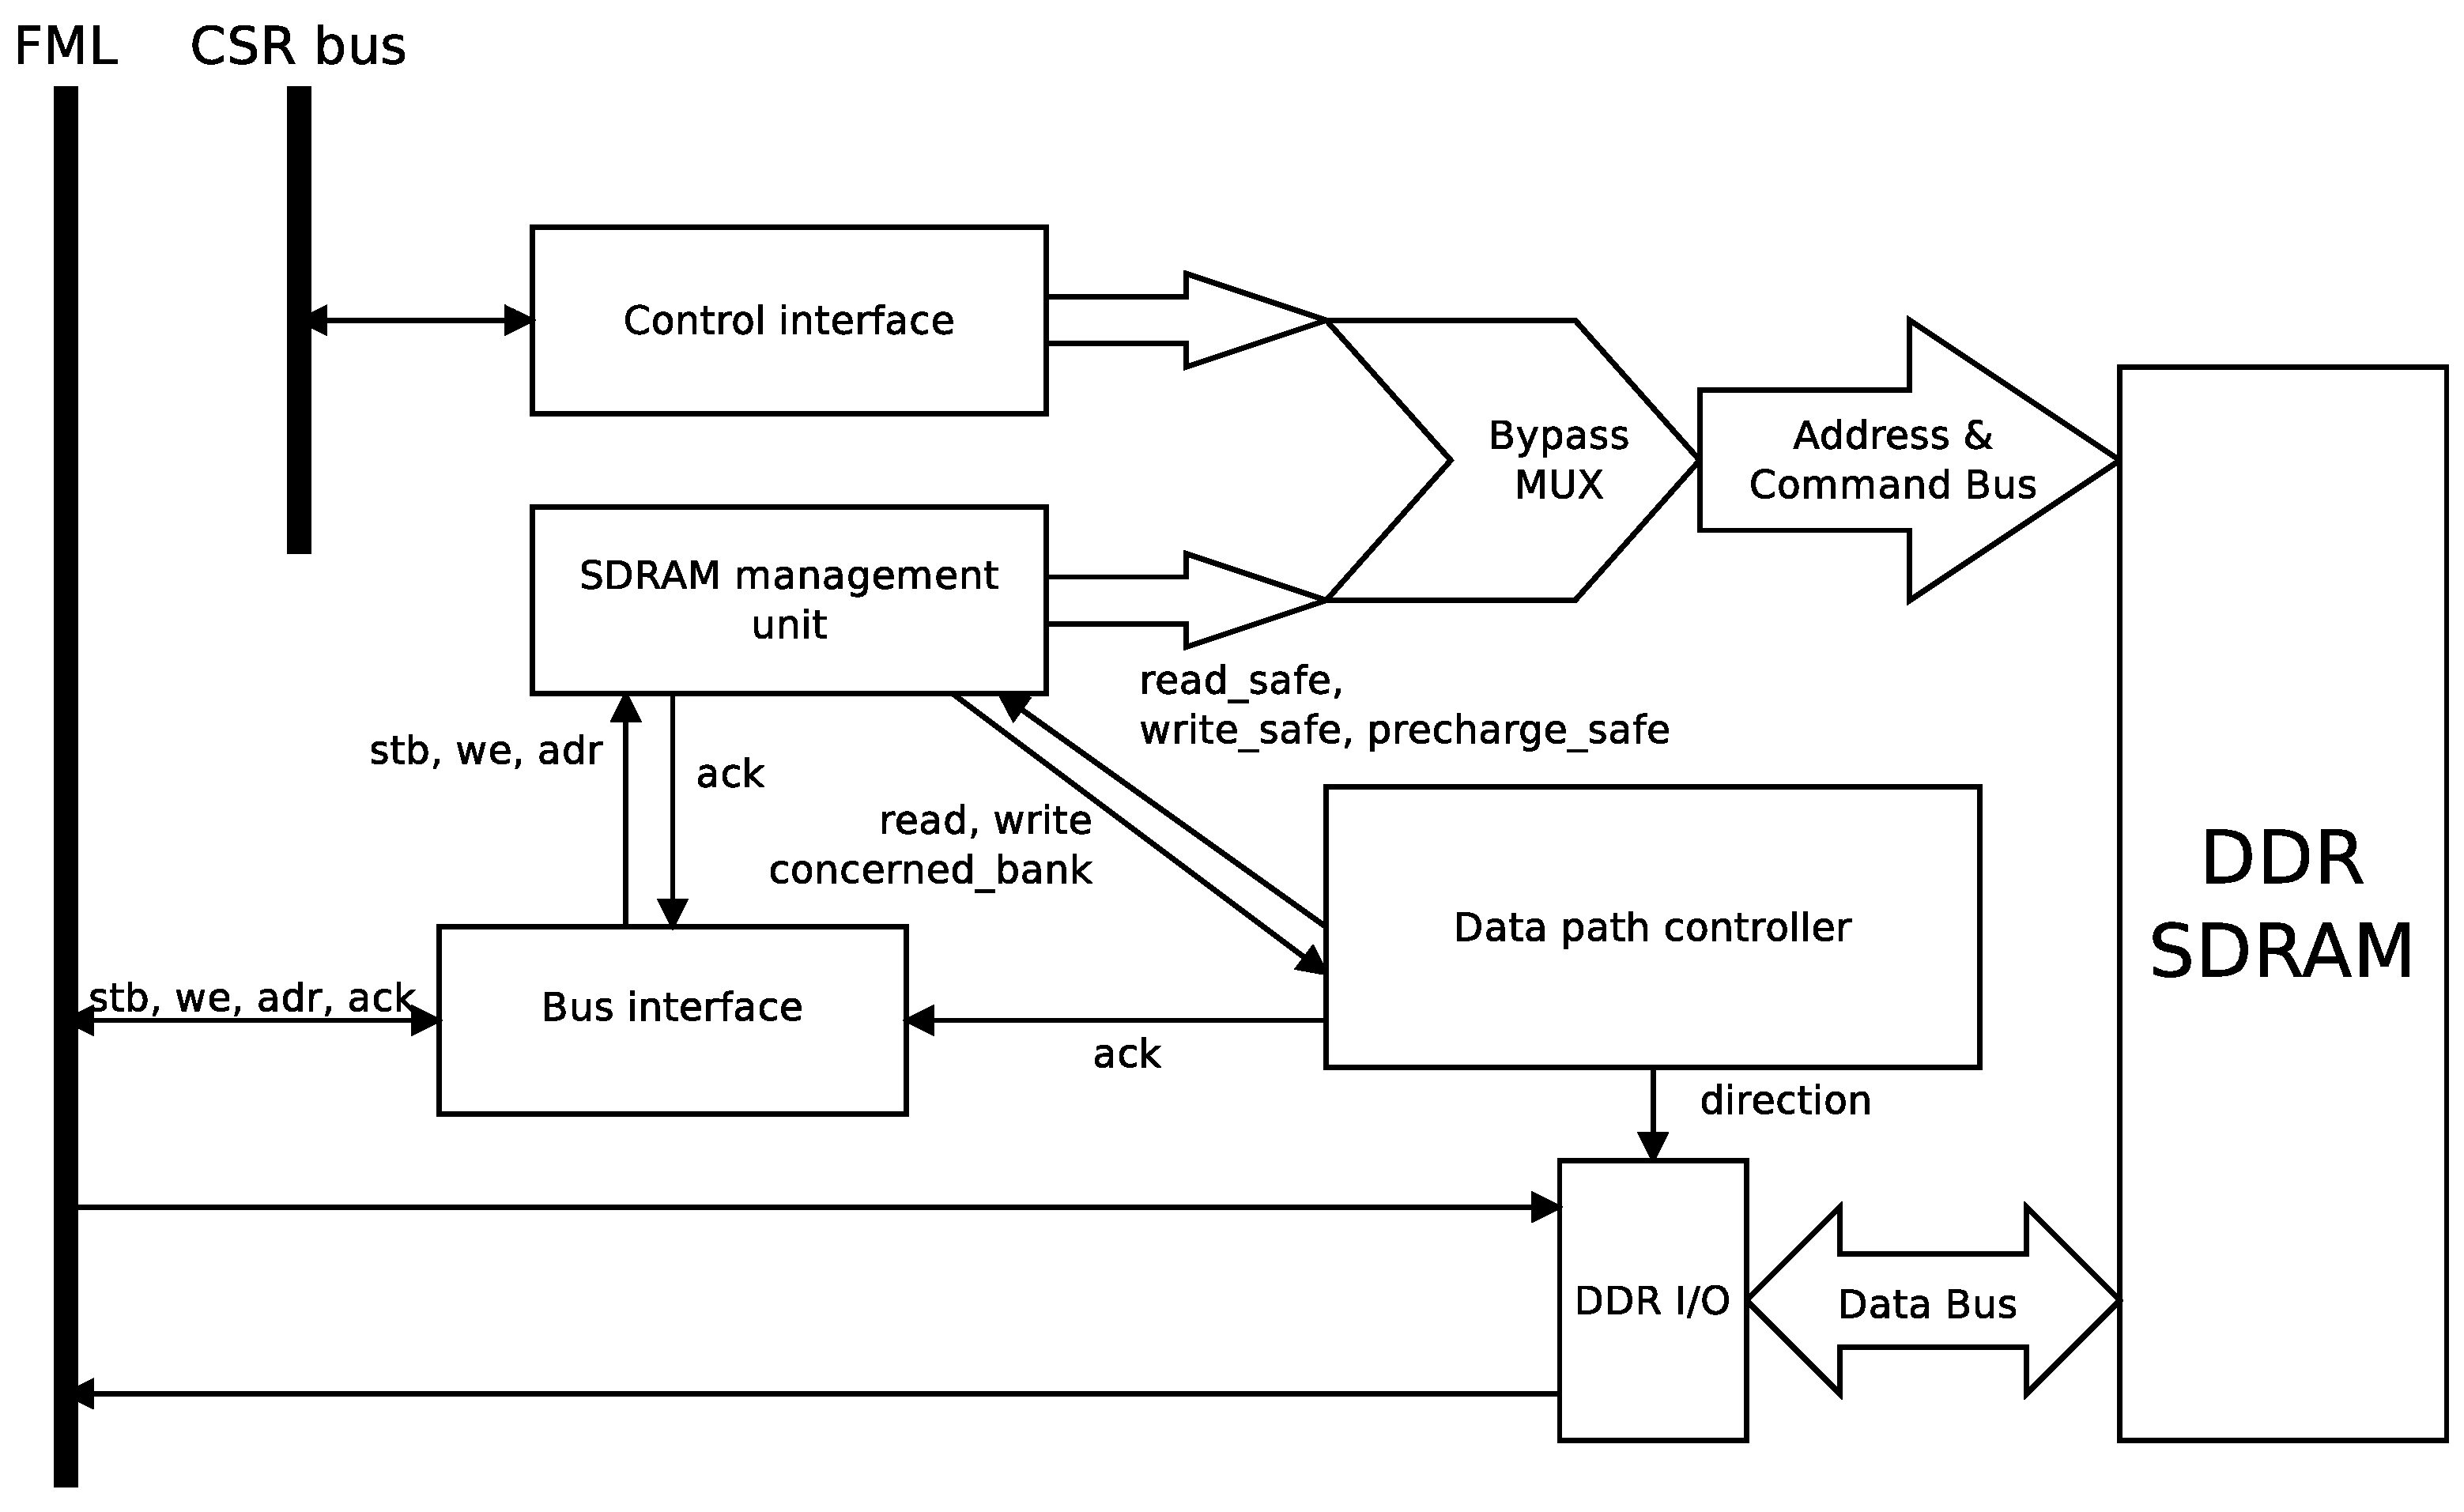
\includegraphics[height=85mm]{hpdmc_block.eps}
\caption{Block diagram of the HPDMC architecture.}\label{fig:hpdmc_block}
\end{figure}

The architecture of the memory controller, dubbed HPDMC (for ``High Performance Dynamic Memory Controller''), is outlined in figure~\ref{fig:hpdmc_block}.

The control interface is used by the system to configure the controller, and also to issue the start-up sequence to the SDRAM. Indeed, SDRAM chips require a sophisticated sequence of commands upon power-up. In many memory controller designs, a hardware finite state machine is used to issue this command sequence. In order to save hardware resources, the system used  here leaves this task to the software, and, for this purpose, includes a ``bypass MUX'' that routes directly a configuration and status register of HPDMC to the SDRAM command and address pins. Once the SoC has run a software routine that sends the correct initialization sequence to the SDRAM, it switches permanently the bypass MUX to the ``SDRAM management unit'' and can use off-chip memory normally.

The SDRAM management unit is a finite state machine that translates the two high-level memory commands ``read burst at address'' and ``write burst at address'' into a series of lower-level commands understandable by the SDRAM chips (precharge bank, select row, read from row, etc.). The management unit is responsible for keeping track of the open rows, detecting page hits, switching rows, and issuing periodic DRAM refresh cycles.

The management unit is connected to the ``data path controller'', that follows the activities performed by the management unit in order to decide the direction of the bidirectional I/O pins (they should be set as outputs for writes and as input for reads). The data path controller is also responsible for sending signals to the management unit that indicate if it is safe to perform certain low-level operations. For example, the \verb!read_safe! signal goes low immediately after a read command is issued, because if another one were sent immediately after, the two resulting bursts would overlap in time and this could not work because there is only one set of data pins. Eventually, the data path controller takes into account the SDRAM write and read latencies to generate an acknowledgement signal when the data is actually there (or needs to be sent to the SDRAM) after a ``read row'' or ``write row'' command has been sent to the SDRAM.

Finally, the bus interface is a piece of glue logic that connects the SoC pipelined memory bus (FML) to the data path controller and the management unit.

HPDMC has been implemented in Verilog HDL, tested and debugged in RTL simulation using a DDR SDRAM Verilog model from Micron, integrated into the SoC, synthesized into FPGA technology, and eventually calibrated and tested by software routines running on the actual hardware.

This design of memory controller, specifically crafted for the Milkymist project and released under the GNU GPL license on the internet, has been picked up by the NASA for a software defined radio project and may be put up onboard the international space station in 2011. Gregory Taylor, Electronics Engineer at the NASA Jet Propulsion Laboratory, wrote:

\textit{While searching for a suitable SDRAM controller for the Jet Propulsion Laboratory's Software-Defined Radio onboard NASA's CoNNeCT experiment, I found S\'ebastien's HPDMC SDRAM controller on OpenCores.org. We needed a controller that was both high performance and well documented. Though the original HPDMC controller was designed for DDR SDRAM with a 32-bit bus, S\'ebastien clearly explained the modifications necessary to adapt the controller to our Single Data Rate, 40-bit wide SDRAM chip. I found the code to be well documented and easy to follow. The performance has met our requirements and the FPGA size requirement is small.}

\textit{The Communication Navigation and Networking Reconfigurable Testbed (CoNNeCT) experiment to be installed onboard the ISS is designed for the next generation of SDRs conforming to the Space Telecommunications Radio Systems (STRS) open architecture standard. The HPDMC controller will likely find its way into one or more loadable waveform payloads in the JPL SDR, and perhaps be used in other NASA projects as well. It may eventually find its way into deep space.}

\section{Performance measurement}
\label{sec:memperf}
\subsection{Introduction}
We wanted to validate and characterize the memory system performance (actual latency and bandwidth) and get an upper bound of of its ability to sustain loads, by extrapolating the maximum bandwidth one could get assuming the memory access time remains constant.

Since the memory performance depends on the particular access pattern that the system makes (because of the controller taking the page mode gamble, we wanted to take the measurements on the real system while it is rendering video effects in order to get an accurate result.

\subsection{Method}
A logic core has been added to the SoC that snoops on the memory bus activity in order to report the average latency and bandwidth.

That logic core exploits properties of the FastMemoryLink signaling in order to reduce its complexity to two counters that measure, for a given time period, the number of cycles during which the strobe and acknowledgement signals are active. Several parameters can then be computed:
\begin{itemize}
\item the \textbf{net bandwidth} carried by the link (based on the amount of data that the link has actually transferred)
\item the \textbf{average memory access time}, which is the time, in cycles, between the request being made to the memory controller and the first word of data being transferred.
\item the \textbf{bus occupancy} which is the percentage of time during which the link was busy and therefore unavailable for a new request.
\end{itemize}

Every FastMemoryLink transaction begins with the assertion of the strobe signal. Then, after one or more wait cycles, the memory controller asserts the acknowledgement signal together with the first word of data being transferred. The next cycle, the strobe signal is deasserted (unless a new transaction begins) while the next word in the burst is being transferred. A new transaction can start with the assertion of the strobe signal even if a burst is already going on (pipelining). See figure~\ref{fig:fmltransactions} for an example.

\begin{figure}
\centering
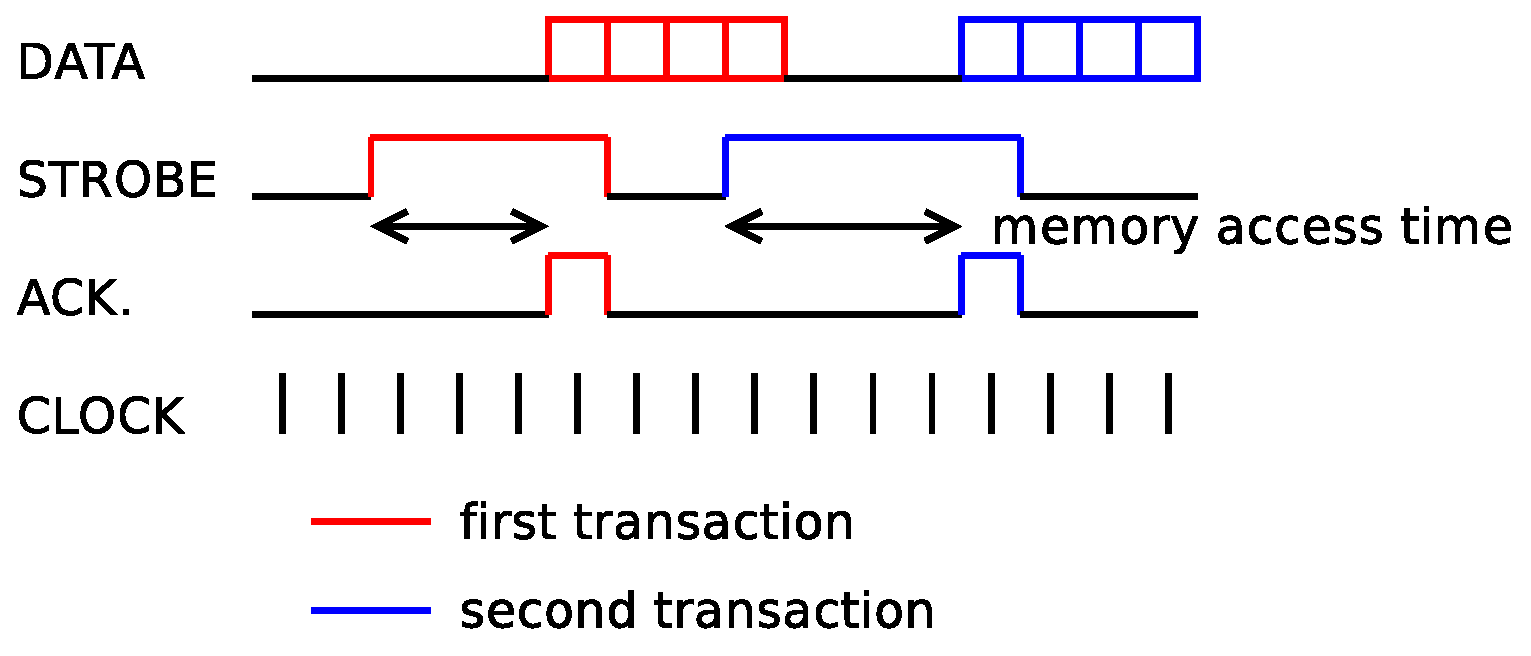
\includegraphics[height=40mm]{fmltransactions.eps}
\caption{FML transactions.} \label{fig:fmltransactions}
\end{figure}

In the equations that follow, these symbols are used:
\begin{itemize}
\item $f$ is the system clock frequency in Hz.
\item $T$ is the time during which the counters have been enabled.
\item $w$ is the width of a FML word in bits.
\item $n$ is the FML burst length.
\item $S$ is the number of cycles during which the strobe signal was active.
\item $A$ is the number of cycles during which the acknowledgement signal was active.
\end{itemize}

\paragraph{Net bandwidth.} By counting the number of cycles for which the acknowledgement signal was active, one gets the number of transactions. Since each transaction carries exactly a burst of data, which is $w \cdot n$ bits in size, the volume of data transferred is given by $w \cdot n \cdot A $. Thus, one can derive the net bandwidth as:
\begin{equation}
\beta = \frac{w \cdot n \cdot A}{T}
\end{equation}

\paragraph{Average memory access time.} On the bus, a master is waiting when the strobe signal is asserted but the acknowledgement signal is not. Therefore, the total number of wait cycles is given by $S-A$. The average memory access time can thus be computed as:
\begin{equation}
\Delta = \frac{S-A}{A}
\end{equation}

\begin{figure}
\centering
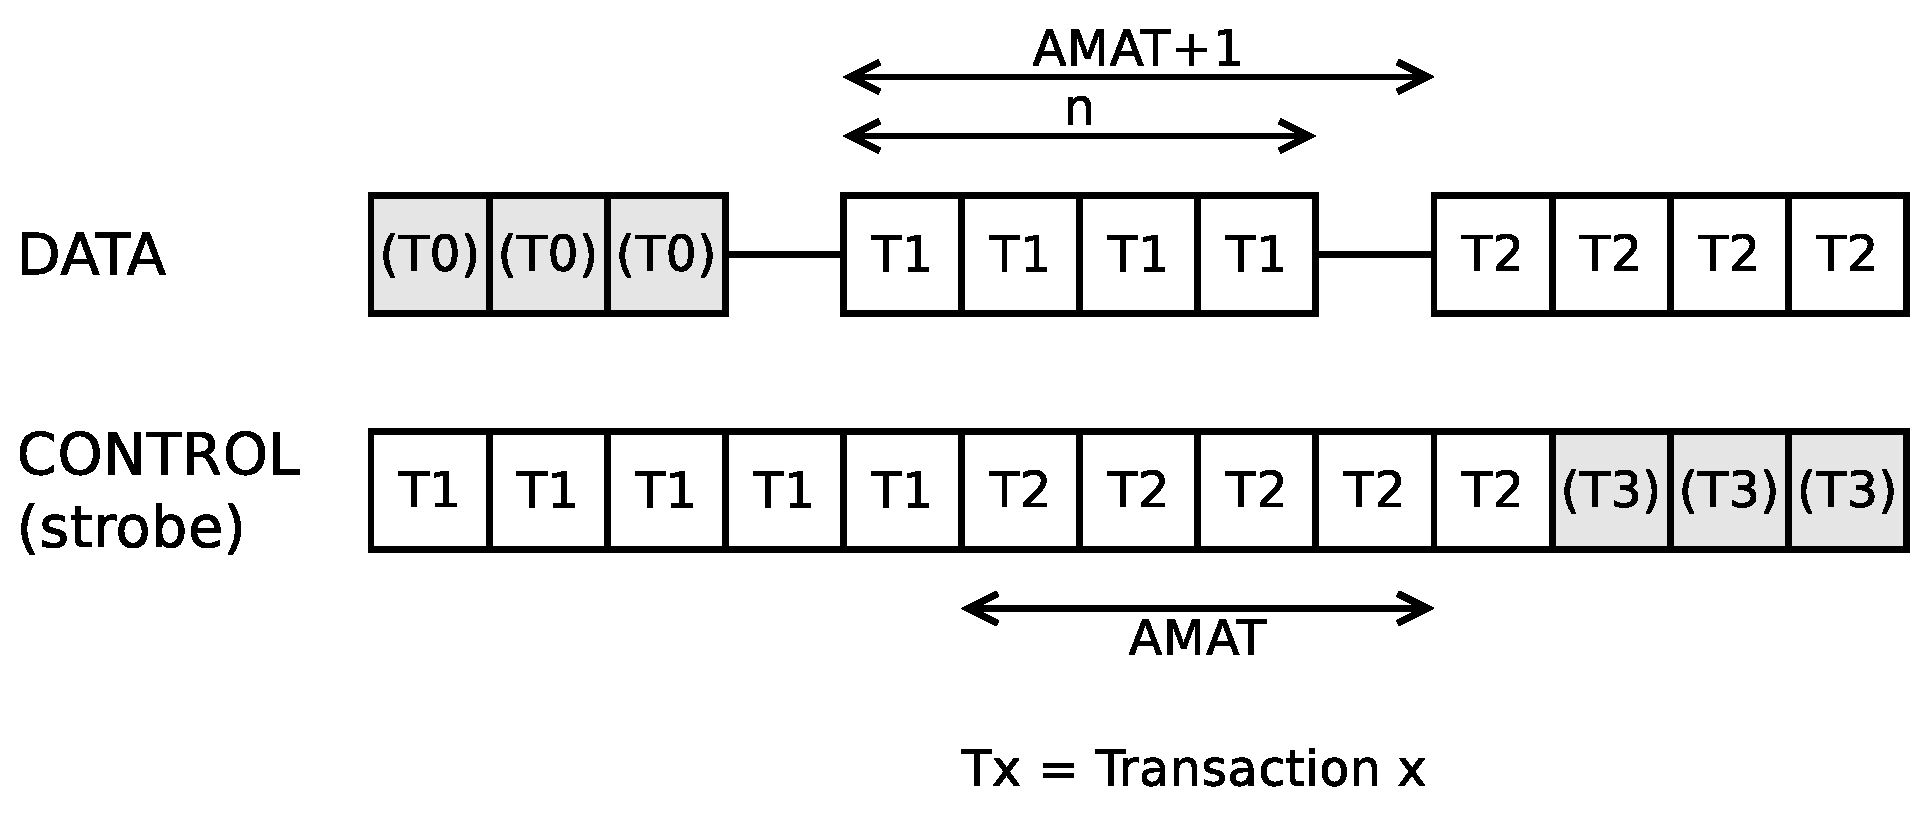
\includegraphics[height=45mm]{fmlmax.eps}
\caption{Maximum utilization of a FML bus.} \label{fig:fmlmax}
\end{figure}

The average memory access time can be used to derive an upper bound on the maximum bandwidth that the memory system can handle. Indeed, FML is a pipelined bus which supports only one outstanding (waiting) transaction, so the case that uses the most bandwidth for a given memory access time is when the strobe signal is always asserted (figure~\ref{fig:fmlmax}) so that a new transaction begins as soon as the first word of the previous trasaction is transferred.

Therefore, only a fraction $\alpha$ of the peak bandwidth $f \cdot w$ can be used at most, and we have:
\begin{equation}
\alpha = \textrm{max}(1, \frac{n}{\Delta+1})
\end{equation}

The maximum bandwidth is:
\begin{equation}
\beta_{max} = \alpha \cdot f \cdot w
\end{equation}

\paragraph{Bus occupancy.} The bus is busy when the strobe signal is asserted. The bus occupancy is therefore given by:
\begin{equation}
\epsilon = \frac{S}{T \cdot f}
\end{equation}

By using this method, a very simple piece of hardware added to the system can yield to the retrieval of interesting information about the performance of the memory system.

\subsection{Results}
Results are summarized in table~\ref{tab:memperformance}. The first line corresponds to a system running the demonstration firmware with the video output enabled at the standard VGA mode of 640x480 at 60Hz (therefore continuously scanning the screen with data from system memory), but not rendering a preset. The other lines represent the results while the demonstration firmware is rendering different MilkDrop presets, still at the same video resolution.

\begin{table}
\centering
\begin{tabular}{|l|l|l|l|l|}
\hline
\textbf{Preset} & $\beta$ & $\epsilon$ & $\Delta$ & $\alpha(\beta_{max})$ \\
\hline
Idle & 293 Mbps & 7 \% & 5.52 & 61 \% (3926 Mbps) \\
\hline
Geiss - Bright Fiber Matrix 1 & 1067 Mbps & 31 \% & 6.58 & 53 \% (3377 Mbps) \\
\hline
Geiss - Swirlie 3 & 1160 Mbps & 34 \% & 6.71 & 52 \% (3320 Mbps) \\
\hline
StudioMusic - Twisted Galaxy & 942 Mbps & 25 \% & 5.94 & 58 \% (3689 Mbps) \\
\hline
Geiss - Spacedust & 1024 Mbps & 30 \% & 6.67 & 52 \% (3338 Mbps) \\
\hline
Geiss - Anomaly 2 & 1127 Mbps & 33 \% & 6.58 & 53 \% (3377 Mbps) \\
\hline
Aderrasi - Candy Avian & 923 Mbps & 27 \% & 6.52 & 53 \% (3404 Mbps) \\
\hline
\end{tabular}
\caption{Memory performance in different conditions (Milkymist 0.5).}\label{tab:memperformance}
\end{table} % TODO: update these results

It is difficult to compare these results to those of other memory controllers as they are usually not published (or not measured at all).

However, two conclusions can be drawn:
\begin{itemize}
\item there are enough occupancy and bandwidth margins for the system to operate at higher resolutions and/or color depths than 640x480 and 16 bits per pixel. The 3.3 Gbps bandwidth requirement that was estimated in section~\ref{sec:memimpl} seems attainable, although challenging.
\item to go further, an ``out-of-order'' memory controller can be envisioned. Such a controller would have a split transaction bus (allowing a larger number of outstanding transactions, thus minimizing the impact that latency has on bandwidth) and would be able to reorder pending memory transactions to maximize the page hit rate.
\end{itemize}

\chapter{SoC interconnect}
\label{ch:intercon}
This chapter explains how the different interconnect busses work, what their features are, why they are there, and how they are communicate with each other.

The general SoC block diagram and its interconnect is outlined in figure~\ref{fig:block}.

\section{General SoC interconnect: the Wishbone bus}
Wishbone~\cite{wishbone} is a general purpose royalty-free SoC bus with open specifications, advocated by the maintainers of the OpenCores.org website.

Wishbone is a synchronous sequential bus with support for variable latency (wait states) through the use of an acknowledgement signal that marks the end of the transaction. Burst modes (automatic transfer of consecutive words) are supported and are configurable on a per-transaction basis (i.e. bursts of arbitrary lengths and single-word transactions can be freely mixed on the same bus). However, there is no pipelining.

Wishbone is used around the SoC's LatticeMico32 CPU core and for simple DMA masters which have modest requirements of bandwidth and of volume of transferred data. As will be explained in Section~\ref{sec:fmlbrg}, connecting DMA masters that transfer small amounts of data (which can fit in the L2 cache) to the same bus as the CPU simplifies dealing with cache coherency issues.

The data width used for the Wishbone bus is 32, yielding a peak bandwidth of 3.2Gbps when the system is running at 100MHz.

\section{Configuration and Status Registers: the CSR bus}
Milkymist uses memory-mapped I/O through configuration and status registers.

If these registers were directly accessed by the Wishbone CPU bus, two problems would arise:
\begin{itemize}
\item Connecting all peripherals on the same Wishbone bus involves large multiplexers and high fanout signals, posing routing and timing problems.
\item Wishbone requires the generation of an acknowledgement signal by each slave core. This signal is useful in many cases, as it supports peripherals with a variable latency. However, configuration and status register files are usually implemented with actual registers (flip flops) or SRAM, which can always be accessed in one clock cycle. Thus, there is no need for variable latency and the acknowledgement signal. Keeping this signal for the configuration and status registers wastes hardware resources and development time.
\end{itemize}

To alleviate these problems, the CSR bus has been developed~\cite{csr} and used in the system through a bus bridge.

The CSR bus is a simpler bus than Wishbone, where all transfers are done in one cycle. It has an interface similar to that of synchronous SRAM, consisting only of address, data in, data out and write enable pins and clocked by the system clock.

A bridge connects the CSR bus to the CPU Wishbone bus, to allow transparent memory-mapped access to the configuration and status registers by the software. This bridge includes registers for all the signals crossing the two busses, relaxing the timing constraints.

\section{High-throughput memory access bus: the FML bus}
FastMemoryLink (FML)~\cite{fml} was co-designed with HPDMC (the memory controller) as a on-chip bus tailored to access SDRAM memories at high speed while keeping the memory controller simple. Its key features are listed below.

\subsection{Variable latency}
SDRAM latency varies a lot depending on the state of the SDRAM at the time the request is issued on the bus. It depends on whether the SDRAM was in the middle of a refresh cycle, whether the bank needs to be precharged, and whether a new row needs to be activated. Therefore, FML provides support for a variable number of wait states, defined by the memory controller, through the use of an acknowledgement signal similar to that of Wishbone.

\subsection{Burst only}
SDRAM is best accessed in burst mode (see subsection~\ref{subsec:fmlburst}).

However, enabling or configuring burst mode is a relatively lengthy and complex operation, requiring a reload of the SDRAM mode register which takes several cycles. Furthermode, supporting multiple burst lengths makes the scheduling of the transfers more complex to avoid ``overlapping'' transfers that would create conflicts at the data pins.

Therefore, in order to greatly simplify the memory controller, all transfers on FML are made using a fixed and pre-defined burst length.

\subsection{Burst reordering}
This was discussed in subsection~\ref{subsec:fmlborder}.

\subsection{Pipelining}
The benefits of this feature have already been discussed in subsection~\ref{subsec:fmlpipe}.

Pipelined requests may come from the same core that issued the initial transfer, or from another core. The FML arbiter would then pipeline the request coming from the other core.

\subsection{Usage}
The data width used for the FML bus is 64, yielding a peak bandwidth of 6.4Gbps when the system is running at 100MHz. This is twice the peak bandwidth of the Wishbone bus. Furthermore, this bus provides a short path to the memory controller, reducing latency and therefore potentially further increasing effective bandwidth, as discussed in Section~\ref{sec:memorywall}.

Peripherals directly connected to FML are typically those which transfer large amounts of data (that would exceed the capacity of the L2 cache presented in Section~\ref{sec:fmlbrg}) and which have high bandwidth requirements (and therefore can take advantage of the bandwidth and latency improvement compared to Wishbone).

In the Milkymist SoC, they are comprised of:
\begin{itemize}
\item the VGA output controller, which needs to continously scan a framebuffer up to several megabytes in size to generate the video signal.
\item the (planned) video input, which writes, every second, dozens of digitized video frames weighting hundreds of kilobytes each.
\item the texture mapping unit (Chapter~\ref{ch:tmu}), which needs to deal with large textures at high speed.
\end{itemize}

\section{Bridging Wishbone to FML}
\label{sec:fmlbrg}
For Wishbone masters (like the CPU) to access SDRAM transparently, it is necessary to bridge the FML bus to the Wishbone bus.

FML is a burst-only bus with a fixed burst length, while with Wishbone, bursts are optional and configured on a per-transaction basis. To be efficient, the bridge must therefore be able to store data and slice it to meet the transfer size requirements of the Wishbone and FML transactions.

A traditional write-back cache with a line length equal to the FML burst length provides an elegant solution to this problem. This cache is referred to as the ``L2 cache'', because, from the CPU point of view, it provides a second level of cache relative to its integrated instruction and data caches.

\section{Cache coherency}
\label{sec:coherency}
\subsection{Coherency issues around the CPU (L1) cache}
The LatticeMico32 CPU (section~\ref{sec:mico32}) uses a write-through cache without hardware coherency. Thus, the following operations must be done by the software to ensure cache coherency:
\begin{itemize}
\item Before reading DMA data from a peripheral using shared memory, the L1 cache should be cleared as it may hold an outdated copy of the data.
\item When writing DMA data to a peripheral using shared memory on the Wishbone bus, no precaution should be taken. The CPU writes go directly to the bus, and end up in the L2 cache or the SDRAM where the peripheral will correctly retreive them.
\end{itemize}

It is noteworthy that the CSR address space is non-cacheable, therefore no cache-related precaution should be taken when reading or writing CSRs.

\subsection{Coherency issues around the Wishbone-FML (L2) cache}
The Wishbone-FML bridge provides very limited support for cache coherency. Cache coherency issues arise because of the masters directly connected to the FML bus:
\begin{itemize}
\item The CPU may read a cached copy of a data that has been modified by a FML master.
\item A FML master may read a value that has been modified by the CPU in the cache (dirty line) but not flushed to the SDRAM.
\item A FML master may update a value in SDRAM but not in the cache. The line may then go dirty, and, when flushed, will erase the value written by the FML master.
\end{itemize}

Because cache coherency is expensive to implement in hardware, the task of managing the coherency of caches has been moved almost entirely to the software. The bridge exposes an interface for the software to invalidate cache lines, flushing them to the SDRAM if they are dirty. On the software side, device drivers should use this interface appropriately when transferring data with hardware units that use shared memory.

The only form of hardware cache coherency the system has is related to the video framebuffer. The VGA signal generator is connected directly to the SDRAM bus, because the framebuffer is continuously scanned and is too large to fit entirely in the cache.

However, it is very common that software modifies only a few pixels on the screen. If there was no hardware cache coherency at all, it would be tricky to implement a software mechanism that flushes the bridge cache at appropriate times. A solution can be to flush the cache every time a pixel or a group of pixels are written (which can be extremely slow if only small regions of the screen are modified at a time). Another solution would be to periodically check if the framebuffer had been modified and flush the cache if it was.

Since those solutions are difficult to implement as they require a significant support from both the operating system and applications, it was chosen to make framebuffer read transactions by the VGA signal generator coherent with respect to the bridge cache. Every time the VGA signal generator fetches a burst of pixels, it first searches the bridge cache. If the data is in the cache, it is used. If not, the VGA signal generator fetches it from SDRAM (but does not replace any cache line).

This also makes it easier to write Milkymist framebuffer drivers within the frameworks of common operating systems, such as Linux (figure~\ref{fig:linux}).

\chapter{Texture mapping unit}
\label{ch:tmu}
High performance texture mapping was perhaps the most challenging and interesting part of the SoC design project. This chapter begins with the design of an efficient algorithm and continues with the hardware implementation of it, and in particular how it was pipelined and how its memory references are handled.

\section{Algorithm}
\subsection{Two-dimensional interpolation}
As outlined in section~\ref{sec:tm}, we need to interpolate linearly on a 2D polygon the X and Y texture coordinates according to known values on the vertices of the polygon.

Traditional GPUs use the triangle as the primitive polygon, because it allows them to draw any other polygon by splitting it into a series of triangles. We do not need such flexibility. For rendering MilkDrop presets, the surface to be drawn is always a mesh of rectangles whose edges are parallel to the borders of the screen (traditional GPUs draw the surface using a triangle decomposition similar to the one shown in figure~\ref{fig:tridec}). We can therefore choose, as the primitive polygon, the rectangle with edges parallel to the borders of the screen, which is much simpler to draw than arbitrary triangles.

\begin{figure}[htp]
\centering
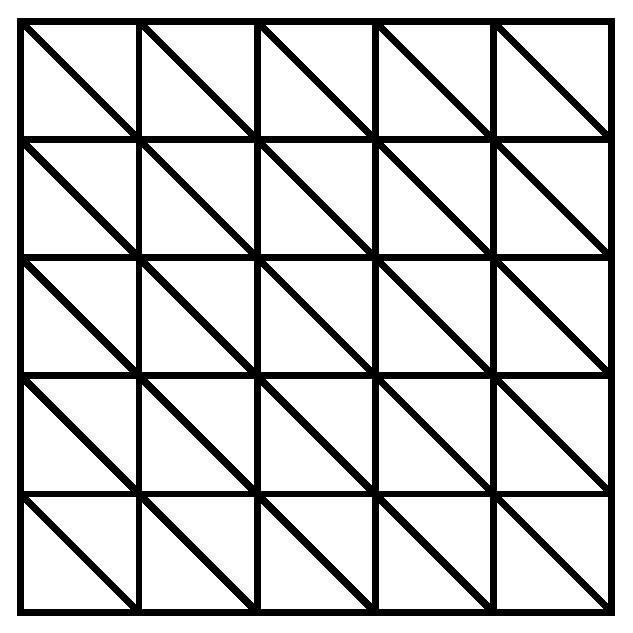
\includegraphics[height=50mm]{tridec.eps}
\caption{Typical decomposition into triangular primitives of the MilkDrop rendering surface.}
\label{fig:tridec}
\end{figure}

We then split the 2D interpolation problem into 1D interpolation problems as follows:
\begin{itemize}
\item The X and Y texture coordinates are interpolated independently.
\item First, each coordinate is interpolated on the vertical edges of the rectangles (vertical interpolation) for each integer value of the ordinate.
\item For each integer value of the ordinate, the results from the vertical interpolation are interpolated again for each integer value of the abscissa (horizontal interpolation). This scans all the pixels within the rectangle.
\end{itemize}
The process is illustrated in figure~\ref{fig:rectinter}.

One could obtain the same result by starting with an horizontal interpolation followed by several vertical interpolations. However, when using a linear scan framebuffer (as Milkymist does), doing it in the proposed way yields output pixels whose memory addresses are consecutive in most cases (except when going to the next ordinate), which works well with the bursty nature of SDRAM accesses (subsection~\ref{subsec:fmlburst}) and the traditional organization of a cache.

\begin{figure}[htp]
\centering
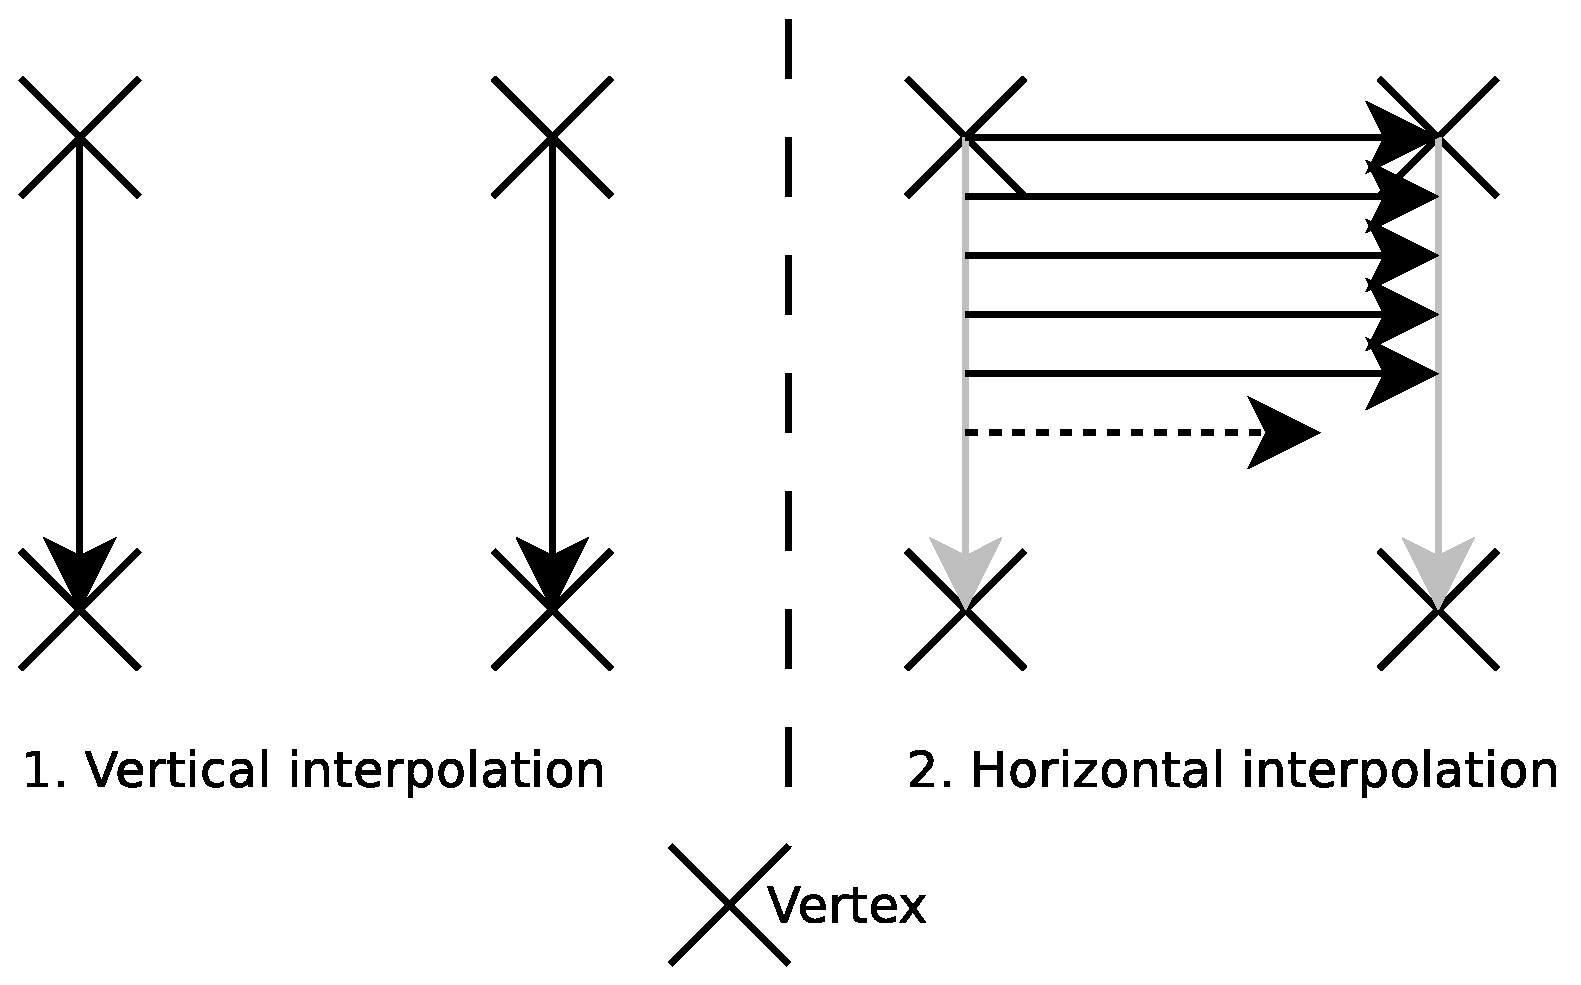
\includegraphics[height=70mm]{rectinter.eps}
\caption{2D linear interpolation on a rectangle.}
\label{fig:rectinter}
\end{figure}

\subsection{One-dimensional interpolation}
The problem now boils down to performing one-dimensional linear interpolations. Given two points $A(x_{0}, y_{0})$ and $B(x_{1}, y_{1})$ with integer coordinates, we need to compute the ordinate $y$ of $M(x, y) \in (AB)$ for all the integer values of $x$ between $x_{0}$ and $x_{1}$. For now, we are not interested in bilinear filtering, so what we actually want is the best integer approximation $[y]$ of $y$ so that the texture is sampled to the nearest pixel.

In figure~\ref{fig:interalgo} we propose a fast and integer-only\footnote{And thus more suited to a resource-constrained hardware implementation.} algorithm, which was inspired by Bresenham's line drawing algorithm~\cite{bresenham}. Without loss of generality, we suppose that $x_{0} \leq x_{1}$ (the points can be reordered if this was not the case). We also suppose that $y_{0} \leq y_{1}$ (it is easy to modify the algorithm to handle the $y_{0} > y_{1}$ case as well\footnote{See the Verilog implementation in Milkymist (cores/tmu2/rtl/tmu2\_geninterp18.v).}).

\begin{figure}
\centering
\begin{boxedminipage}{13cm}
\begin{math}
Dy \leftarrow y_{1} - y_{0} \\
Dx \leftarrow x_{1} - x_{0} \\
Q \leftarrow Dy / Dx \footnote{/ is the integer division operator} \\
R \leftarrow Dy \% Dx \footnote{\% is the integer modulo operator}  \\
x \leftarrow x_{0} \\
\hspace{0cm} [y] \leftarrow y_{0} \\ % WA: latex doesn't like lines starting with [
e \leftarrow 0 \\
\textrm{result(x)} \leftarrow [y] \\
\textrm{\textbf{while}~} x < x_{1} \\
\textrm{~~~~~} x \leftarrow x + 1 \\
\textrm{~~~~~} [y] \leftarrow [y] + Q \\
\textrm{~~~~~} e \leftarrow e + R \\
\textrm{~~~~~\textbf{if}~} 2\cdot e > Dx \\
\textrm{~~~~~~~~~~} [y] \leftarrow [y] + 1 \\
\textrm{~~~~~~~~~~} e \leftarrow e - Dx \\
\textrm{~~~~~\textbf{end}} \\
\textrm{~~~~~result(x)} \leftarrow [y] \\
\textrm{\textbf{end}}
\end{math}
\end{boxedminipage}
\caption{One-dimensional linear interpolation algorithm.}
\label{fig:interalgo}
\end{figure}

The correctness of the algorithm lies in the fact that every time the result is being written, those conditions are verified (from which it can be derived that $[y]$ is the best integer approximation of $y$):
\begin{enumerate}
\item $|e| \leq \frac{Dx}{2}$ (which implies $|\frac{e}{Dx}| \leq \frac{1}{2}$)
\item The perfect (rational) interpolated value $y$ is equal to $y = [y] + \frac{e}{Dx}$.
\end{enumerate}

These conditions can be proven true by recursion:
\begin{enumerate}
\item For $x = x_{0}$, $e = 0$ therefore $|e| \leq \frac{Dx}{2}$. Let us now suppose that the hypothesis is true for a certain value of $x \geq x_{0}$, and prove that it is true for $x+1$.

The instructions that affect $e$ between two consecutive values of $x$ are $e \leftarrow e + R$ and, if $2\cdot e > Dx$, $e \leftarrow e - Dx$.

After the first instruction:
\begin{itemize}
\item if $e$ was negative or zero, we have $-\frac{Dx}{2} \leq e < Dx < \frac{3 \cdot Dx}{2} $ (because $0 \leq R < Dx$ and the recursion hypothese).
\item if $e$ was positive, it was inferior or equal to $\frac{Dx}{2}$ (because of the recursion hypothese), therefore we have $0 < e < \frac{3 \cdot Dx}{2} $.
\end{itemize}
After the second instruction, if we had $e > \frac{Dx}{2}$, we'll have $e < \frac{3 \cdot Dx}{2} - Dx$. Therefore, $e \leq \frac{Dx}{2}$. $\Box$

\item We need to prove that every time the result is being written, the following equation is verified:
\begin{equation}
\hspace{0cm} [y] + \frac{e}{Dx} = y_{0} + \frac{y_{1}-y_{0}}{x_{1}-x_{0}} \cdot (x - x_{0})
\end{equation}
For $x = x_{0}$, $[y] + \frac{e}{Dx} = y_{0}$, so the equation is verified. Let us now suppose that it is verified for a certain value of $x \geq x_{0}$, and prove that it is true for $x+1$.

It can be noted that the instructions within the ``if'' do not change the value of $[y] + \frac{e}{Dx}$. The only instructions that change the result between two consecutive values of $x$ are $[y] \leftarrow [y] + Q$ and $e \leftarrow e + R$. Therefore, after the loop iteration, we have:
\begin{equation}
\hspace{0cm} [y] + \frac{e}{Dx} = y_{0} + \frac{y_{1}-y_{0}}{x_{1}-x_{0}} \cdot (x - x_{0}) + Q + \frac{R}{Dx}
\end{equation}
\begin{equation}
\hspace{0cm} [y] + \frac{e}{Dx} = y_{0} + \frac{y_{1}-y_{0}}{x_{1}-x_{0}} \cdot (x - x_{0}) + \frac{y_{1}-y_{0}}{x_{1}-x_{0}} \\
\end{equation}
\begin{equation}
\hspace{0cm} [y] + \frac{e}{Dx} = y_{0} + \frac{y_{1}-y_{0}}{x_{1}-x_{0}} \cdot ((x + 1) - x_{0})
\end{equation}
$\Box$
\end{enumerate}

\subsection{Bilinear filtering}
\label{subsec:bilfpformat}
As outlined in section~\ref{sec:tm}, bilinear filtering is needed to obtain good rendering results.

We will therefore try to improve the previous algorithm so that we get a more precise, non-integer interpolation result. Preferably, the result should be in fixed point format so that it can be easily handled for the actual filtering stage (weighted average of adjacent pixels colors).

The first thing that comes to mind is to try to use the error value $\frac{e}{Dx}$. However, this would require an integer to fixed point division to be performed at each interpolated result (the horizontal interpolation alone would require two such operations per pixel), which is expensive.

A more elegant solution consists in multiplying all the texture coordinates by a power of 2, noted S (this is an inexpensive operation, as it can be implemented with a bit shift). Since the interpolation process is linear, the outputs are also multiplied by S --- but the precision is increased. In other words, the output of the interpolation stages comes directly in fixed point format, with $log_{2}(S)$ digits after the radix point.

Figure~\ref{fig:filtfromfp} illustrates how the bilinear filtering is done using the fixed point texture coordinates. The texture coordinates are noted X.i, X.f, Y.i and Y.f, with ``i'' denoting the integer part of the fixed point number (bits before the radix point) and ``f'' denoting the fractional part (bits after the radix point).

\begin{figure}[htp]
\centering
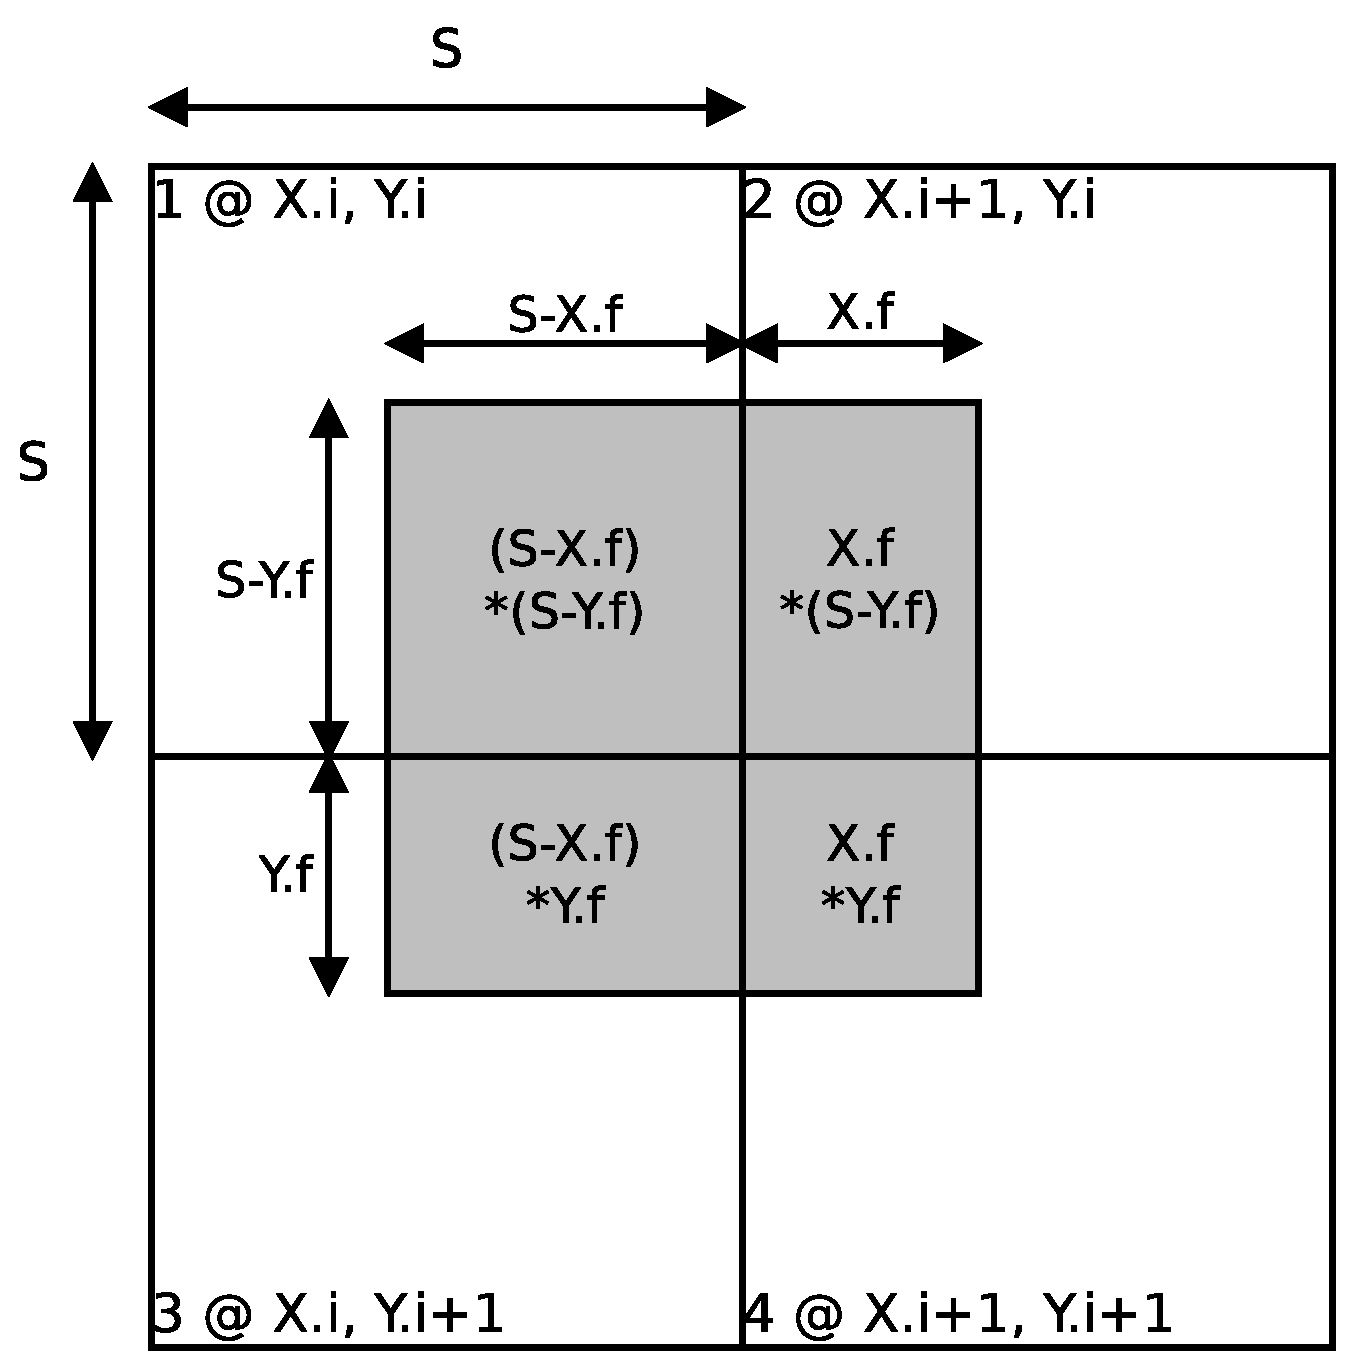
\includegraphics[height=85mm]{filtfromfp.eps}
\caption{Bilinear filtering using the fixed point texture coordinates.}
\label{fig:filtfromfp}
\end{figure}

The weights in the average should be proportional to the surface that the texel to be sampled with non-integer coordinates (the grey box on the figure) covers in each of the real texture pixels (numbered 1 to 4 on the figure). Thus, if $c_{1}$, $c_{2}$, $c_{3}$ and $c_{4}$ are respectively the color vectors of the texture pixels 1 to 4 and $c$ is the color vector of the result, we have:
\begin{equation}\label{eq:bfilter}
c = \frac{(S-X.f)(S-Y.f) \cdot c_{1} + X.f(S-Y.f) \cdot c_{2} + (S-X.f)Y.f \cdot c_{3} + X.fY.f \cdot c_{4}}{S^{2}}
\end{equation}

Since we are working with the RGB565 color format, having more than 6 extra bits of precision would not make a difference for the filtering. Therefore, we choose $S = 2^{6} = 64$.

\section{Performance considerations}
\subsection{Context}
\label{subsec:perfcontext}
To motivate the implementation choice of the texture mapping, we will study its execution time in the following  situation:
\begin{itemize}
\item The size of the source (texture) and destination pictures is 512x512.
\item The size of the primitive rectangles is 16x16.
\item We need at least 120 runs per second. Indeed, the renderer needs to distort the image, include live video, scale it, and apply the video echo effect 30 times per second (subsection~\ref{subsec:mdprinciple}). We therefore have approximately 8 ms of processing time at most (which corresponds to 31 megapixels per second). This is a very optimistic estimate: since scaling, inclusion of live video and the video echo effect work with resolutions greater than 512x512, these processes are expected to take more time than the 512x512 $\rightarrow$ 512x512 distortion.
\item The system clock is 100MHz.
\item The $2\cdot e > Dx$ test is always false (which is optimistic).
\item We optimistically do not take into account the extra instructions needed to handle interpolations with a negative slope ($y_{0} > y_{1}$).
\end{itemize}

For a software implementation, we use the cost estimates of table~\ref{tab:swcost}.

\begin{table}
\centering
\begin{tabular}{|l|l|}
\hline
\textbf{Operation} & \textbf{Cost} \\
\hline
Addition or subtraction & 1 cycle \\
\hline
Multiplication & 2 cycles \\
\hline
Division or modulo & 32 cycles \\
\hline
Bit shift & 1 cycle \\
\hline
Test (<, >, =, etc.) & 1 cycle \\
\hline
Conditional jump & 3 cycles \\
\hline
Assignment & free (which is optimistic) \\
\hline
Reading or writing to the framebuffer & 2 cycles \\
\hline
\end{tabular}
\caption{Estimates of the cost of common software operations.}\label{tab:swcost}
\end{table}

\subsection{Execution time of the interpolation algorithm}
For each 1D interpolation with n steps, we need the amount of time detailed in table~\ref{tab:intertime}. The steps are in the same order as in figure~\ref{fig:interalgo}.

\begin{table}
\centering
\begin{tabular}{|l|l|}
\hline
\textbf{Operation} & \textbf{Cycles} \\
\hline
2 subtractions & $2$ \\
\hline
Division & $32$ \\
\hline
Modulo & $32$ \\
\hline
Test & $n$ \\
\hline
Conditional jump & $3 \cdot n$ \\
\hline
3 additions & $3 \cdot n$ \\
\hline
Bit shift (multiply by 2) & $n$ \\
\hline
Test & $n$ \\
\hline
Conditional jump & $3 \cdot n$ \\
\hline
\textbf{Total} & $66 + 12 \cdot n$ \\
\hline
\end{tabular}
\caption{Detailed estimate of the execution time of the interpolation algorithm.}\label{tab:intertime}
\end{table}

\subsection{Total execution time}
Using the above formula with $n=15$, we can compute an estimate of the execution time of a software implementation (table~\ref{tab:swtmutime}).

1D interpolations need to be done twice, once for each texture coordinate.

The number of framebuffer reads is computed by considering that for each pixel written to the 512x512 destination picture, 4 pixels must be read from the source picture.

The cost of bilinear filtering is computed, for each destination pixel, with 4 subtractions, 8 multiplications, 4 additions and 1 bit shift times 3 color channels, which yields 75 cycles. This is optimistic as it does not take into account the time needed to decode the fixed point format.

\begin{table}
\centering
\begin{tabular}{|l|l|l|}
\hline
\textbf{Operation} & \textbf{Cycles} & \textbf{Time} \\
\hline
Vertical interpolation & 503808 & 5 ms \\
\hline
Horizontal interpolation & 8060928 & 81 ms \\
\hline
Framebuffer reads & 2097152 & 21 ms \\
\hline
Bilinear filtering & 19660800 & 197 ms \\
\hline
Framebuffer writes & 524288 & 5 ms \\
\hline
\textbf{Total} & 30846976 & 308 ms \\
\hline
\end{tabular}
\caption{Optimistic estimate of the execution time of software texture mapping.}\label{tab:swtmutime}
\end{table}

According to this (yet optimistic) estimate, it becomes clear that a software implementation could not suffice, as the required performance is 8 ms. Even the vertical interpolation can hardly be implemented in software, as it would use alone more than 60\% of the CPU power (which is needed for other tasks). We need an overall speedup by a factor of more than 40, using hardware acceleration.

\section{Pipelined hardware implementation}
\subsection{Strategy}
\label{subsec:tmustrategy}
Given the performance constraints and the slowness of software implementations, we decided to implement the complete texture mapping process in hardware.

It is expected that the memory latency for reading the framebuffer would be a performance-limiting factor. Instead of trying to alleviate its effects by using complex and potentially resource-intensive techniques such as advanced prefetching or non-blocking caches, we simply use a direct-mapped blocking texel cache providing simplicity and fast hit times, and design the rest of the mapping unit so that the memory read latency becomes the \textit{only} limiting factor.

With a direct-mapped texel cache having a hit rate of 90\%, a hit time of 1 cycle and a miss penalty of 9 cycles, the average memory access times is 1.8 cycles. With a 100MHz system clock, such a cache has a throughput of 55 megapixels per second, well above the optimistic estimate made in subsection~\ref{subsec:perfcontext}.\footnote{This is a quick estimate assuming a normal cache that does not support bilinear filtering. To implement bilinear filtering, the situation is more complex as the cache needs to look up 4 pixels at once. This will be discussed in subsection~\ref{subsec:texelcache}.}

To make sure that the memory access time is the only limiting factor, it was chosen that the rest of the system should be designed to support a throughput of approximately one output pixel per clock cycle. This heuristic was influenced by the fact that it corresponds to a spatial implementation of the algorithm (i.e. with little or no time-based resource sharing of the hardware components) but does not require resource-intensive duplication of large hardware units either. A spatial implementation requires more area than a time-shared one, but it is simpler to understand, and needs fewer multiplexers and is less prone to routing congestions, making it easier to achieve timing closure in FPGAs.

A deeply pipelined implementation of the texture mapping algorithm was thus chosen, whose block diagram is depicted in figure~\ref{fig:tmublock}. Many of the stages have internal pipeline sub-stages, and they are detailed below.

\begin{figure}[htp]
\centering
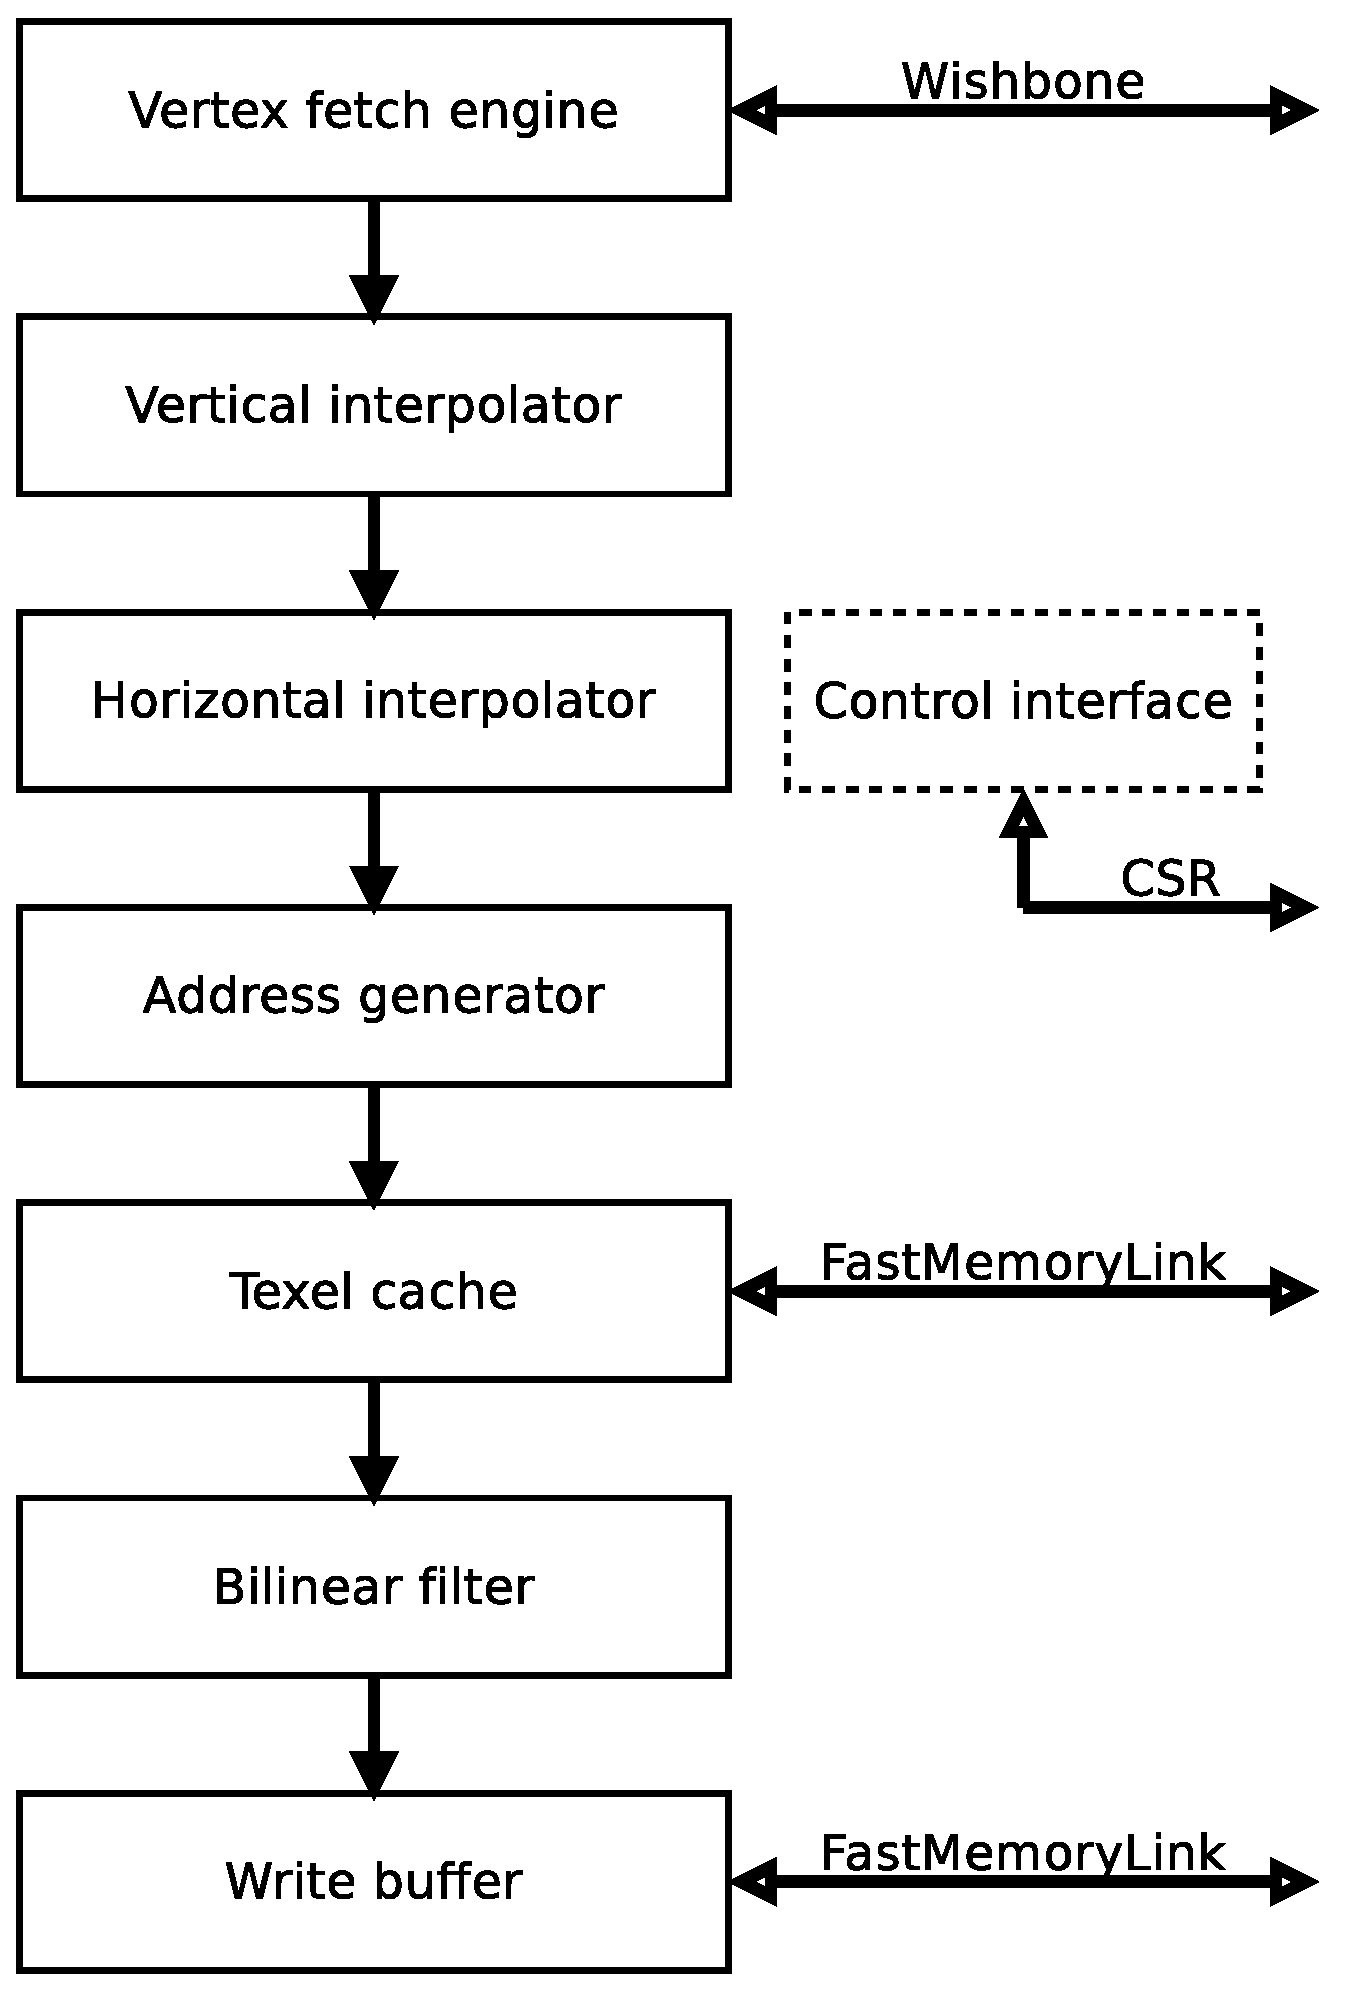
\includegraphics[height=165mm]{tmublock.eps}
\caption{Block diagram of the texture mapping unit architecture.}
\label{fig:tmublock}
\end{figure}

\subsection{Vertex fetch engine}
There is not much to say about this stage, which is a straightforward finite state machine-based Wishbone bus master that fetches the texture coordinates of each vertex from the system memory, and sends them down the pipeline to the vertical interpolator.

The vertex fetch engine is connected to the lower-bandwidth Wishbone bus because this saves resources compared to FML (which has a wider datapath) and makes it easier to handle cache coherency issues (section~\ref{sec:coherency}).

\subsection{Interpolators}
The horizontal and vertical interpolators are both implemented in the same way. They are vector interpolators, which contain two scalar interpolators (figure~\ref{fig:vectinter}, one for each texture coordinate). Each scalar interpolator contains additional internal pipeline sub-stages, as described in figure~\ref{fig:pipeinter}.

The vertical interpolator contains two vector interpolators, one for each vertical edge of the rectangle.

\begin{figure}[htp]
\centering
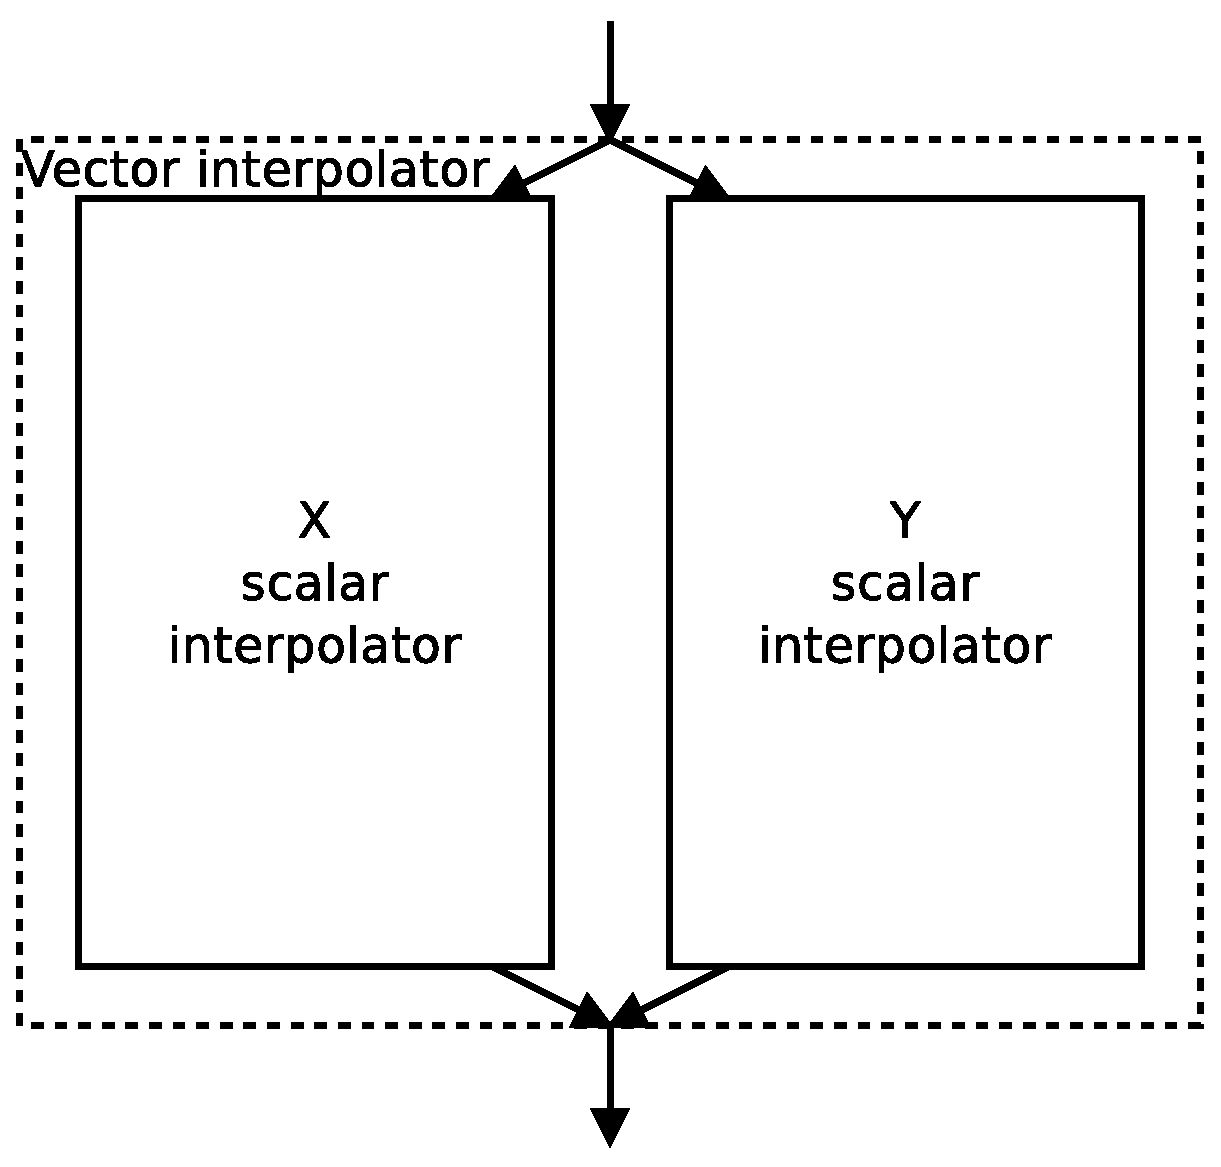
\includegraphics[height=70mm]{vectinter.eps}
\caption{Vector interpolator.}
\label{fig:vectinter}
\end{figure}

\begin{figure}[htp]
\centering
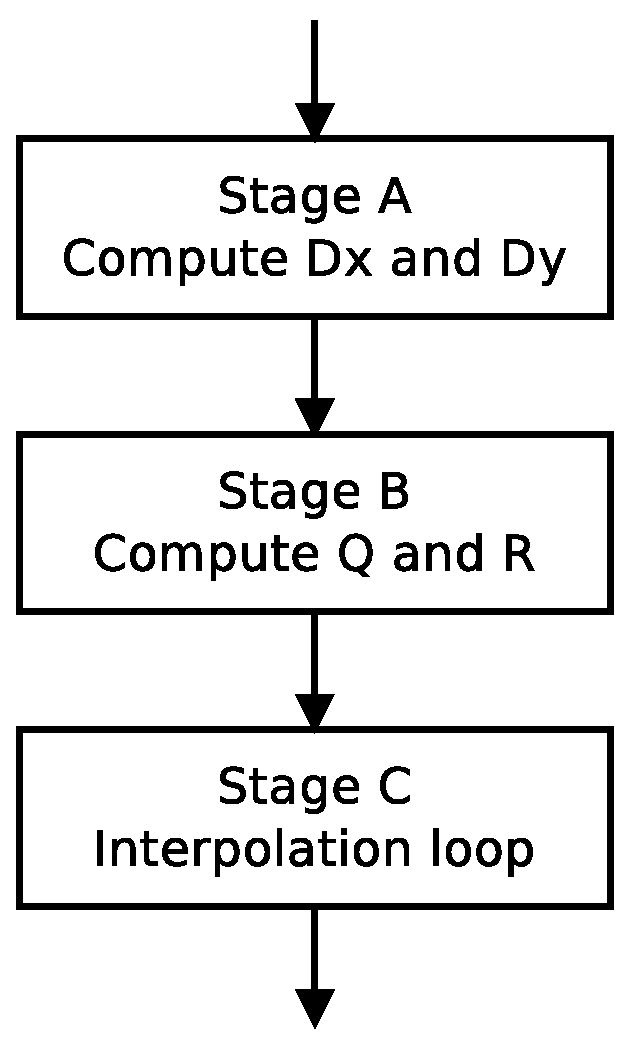
\includegraphics[height=85mm]{pipeinter.eps}
\caption{Pipelined scalar interpolator.}
\label{fig:pipeinter}
\end{figure}

\subsubsection{Stages of the scalar interpolator}
\paragraph{Stage A: Dx and Dy computation.} This stage computes the two differences $y_{1} - y_{0}$ and $x_{1} - x_{0}$. It is based on simple registered arithemetic combinatorial functions, which compute the two differences in one clock cycle.

\paragraph{Stage B: Q and R computation.} The next operation is to perform the Euclidian division of Dy by Dx. The hardware does so by using the restoring division method~\cite{restdiv}, which takes as many cycles as there are quotient digits (our implementation has 18).

In order to keep the resource usage low, the divider is not pipelined. After operands are sent to it, it will stall transmissions from the upstream stage for several cycles until the division is complete.

\paragraph{Stage C: Interpolation loop.}
Finally, the core of the algorithm (the ``while'' loop from figure~\ref{fig:interalgo}) is implemented in the last stage. This unit receives the Q and R values from the dividers, as well as the start $y_{0}$ value and the range $x_{0}$ to $x_{1}$ (which are forwarded through the previous stages). It then sends the series of interpolated values $[y]$ for $x_{0} \leq x < x_{1}$.

The throughput of the stage is one interpolation point per clock cycle. While the interpolation is taking place, transmission of new parameters from the upstream stage is stalled. This justifies the choice of a slow but low-area restoring divider in stage B: with a typical rectangle size of 16, the processing times of the interpolation loop and of the divider are roughly the same, making the pipeline balanced.

\subsection{Clamping/wrapping}
This unit processes interpolated texture points whose coordinates are beyond the boundaries of the texture (i.e. they are negative or exceed the texture's horizontal or vertical resolution).

There are two, selectable, ways of dealing with them:
\begin{itemize}
\item \textit{clamping}, which consists in replacing an out-of-range coordinate with 0 (if it was negative) or with the horizontal or vertical resolution of the texture minus one (if it was too large).
\item \textit{wrapping}, which repeats the texture and consists in computing the positive modulo of each coordinate with respect to the horizontal or vertical texture resolution. In order to avoid using an expensive fast divider, only textures whose sizes are a power of 2 are supported for wrapping. This enables the replacement of the divider with a bitwise AND operation, which is way less expensive. The problem of negative texture coordinates is solved by simply masking out the sign bit, which yields the correct result as the coordinates are represented in two's complement format.
\end{itemize}

This stage is implemented by simple arithmetic combinatorial functions, which are registered and pipelined on two sub-stages to meet timing requirements.

\subsection{Address generator}
The address generator is a simple arithmetic circuit that turns the floating point texture coordinates into the four memory addresses of the pixels they cover, and the destination coordinate into the corresponding memory address in the destination framebuffer. It is pipelined on three sub-stages to meet timing goals.

The formula used to convert a coordinate $(x,y)$ into a pixel address $A$ within a 16bpp framebuffer starting at $A_{base}$ and with an horizontal resolution $H$ is the following:
\begin{equation}\label{eq:fbadr}
A = A_{base} + (H \cdot y + x) \cdot 2
\end{equation}

\subsection{Texel cache}
\label{subsec:texelcache}
\subsubsection{Presentation}
Once the addresses of the four texture pixels have been computed, the next step is to retrieve data from the memory. This should be done fast: to meet the performance goal of 31 megapixels per second at the output of the texture mapping unit, the texel cache must be able to fetch at least 124 megapixels per second. This is, on average, at least 1.24 pixel per clock cycle with a 100MHz system clock.

In consistence with the heuristic made at subsection~\ref{subsec:tmustrategy} that consists in designing the system for a performance of one output pixel per clock cycle in the absence of memory read delays, the texel cache should be able to service the four request ports (called \textit{channels}) in one clock cycle if all the channels hit the cache.

Channel are numbered as follows (see figure~\ref{fig:bilinear}):
\begin{itemize}
\item Channel 1 fetches the \textit{base} pixel, that is to say, the pixel at the coordinates obtained by flooring the non-integer texture coordinates. It is always active.
\item Channel 2 fetches the pixel at the right of the base pixel. It is active when the X texture coordinate has a non-zero fractional part.
\item Channel 3 fetches the pixel at the bottom of the base pixel. It is active when the Y texture coordinate has a non-zero fractional part.
\item Channel 4 fetches the pixel at the bottom-right of the base pixel. It is active when both the X and Y texture coordinate have a non-zero fractional part.
\end{itemize}

\subsubsection{Separate vs. shared caches}
The obvious solution seems have one separate cache per channel. However, this solution is not optimal in terms of speed and memory efficiency. For example, let us take the case when the texture mapping consists in zooming the texture by a factor of 2 (the texture coordinates at each vertex are the vertex coordinates divided by 2). Assuming an empty cache at the beginning, the sequence of events is as follows:
\begin{enumerate}
\item The interpolated fixed-point texture coordinates are (0, 0). Channel 1 misses its cache for a fetch of the pixel at (0, 0). Since the coordinates are integer, channels 2, 3 and 4 are idle and do not need to fetch data.
\item The texture coordinates become (0.5, 0). Channel 1 hits its cache for the pixel at (0, 0). However, channel 2 misses its cache for the pixel at (1, 0) and a new memory request needs to be performed, even though the pixel at (1, 0) is in the cache of channel 1 (it was part of the burst that fetched the (0, 0) pixel). Channels 3 and 4 are idle, since the Y coordinate is integer.
\end{enumerate}
The problem repeats every time the X texture coordinate crosses a memory burst boundary, and is also present in the Y direction with channels 3 and 4. In total, the texel cache uses \textit{four times} as much memory bandwidth as it would use if it were able to share data between the channels' respective caches.\footnote{Assuming at least two complete horizontal lines of pixels from a primitive rectangle fit in the cache, which is generally the case.} Zooming (locally or globally) is a very common operation, so the issue needs to be addressed.

A more efficient solution, which has been retained, consists therefore in having a single multi-ported data store.

\subsubsection{Implementation}
Our implementation is based on the traditional direct-mapped cache, but using quad-port SRAM for the data and tag stores. Quad-port SRAM can be mapped to FPGA technologies at a moderate cost by using two primitive dual-port SRAMs in which the data is replicated. During normal operation (hits), each port serves one channel, and, when refilling the cache on a miss, reading is disabled and two of the ports (one per primitive dual-port SRAM) are used to feed the data into the RAMs.

A simplified block diagram of the texel cache is given in figure~\ref{fig:tcarch}. This block diagram does not include all of the logic needed to handle pipeline stalls and lacks the ``valid'' bits of the tags.

\begin{figure}[htp]
\centering
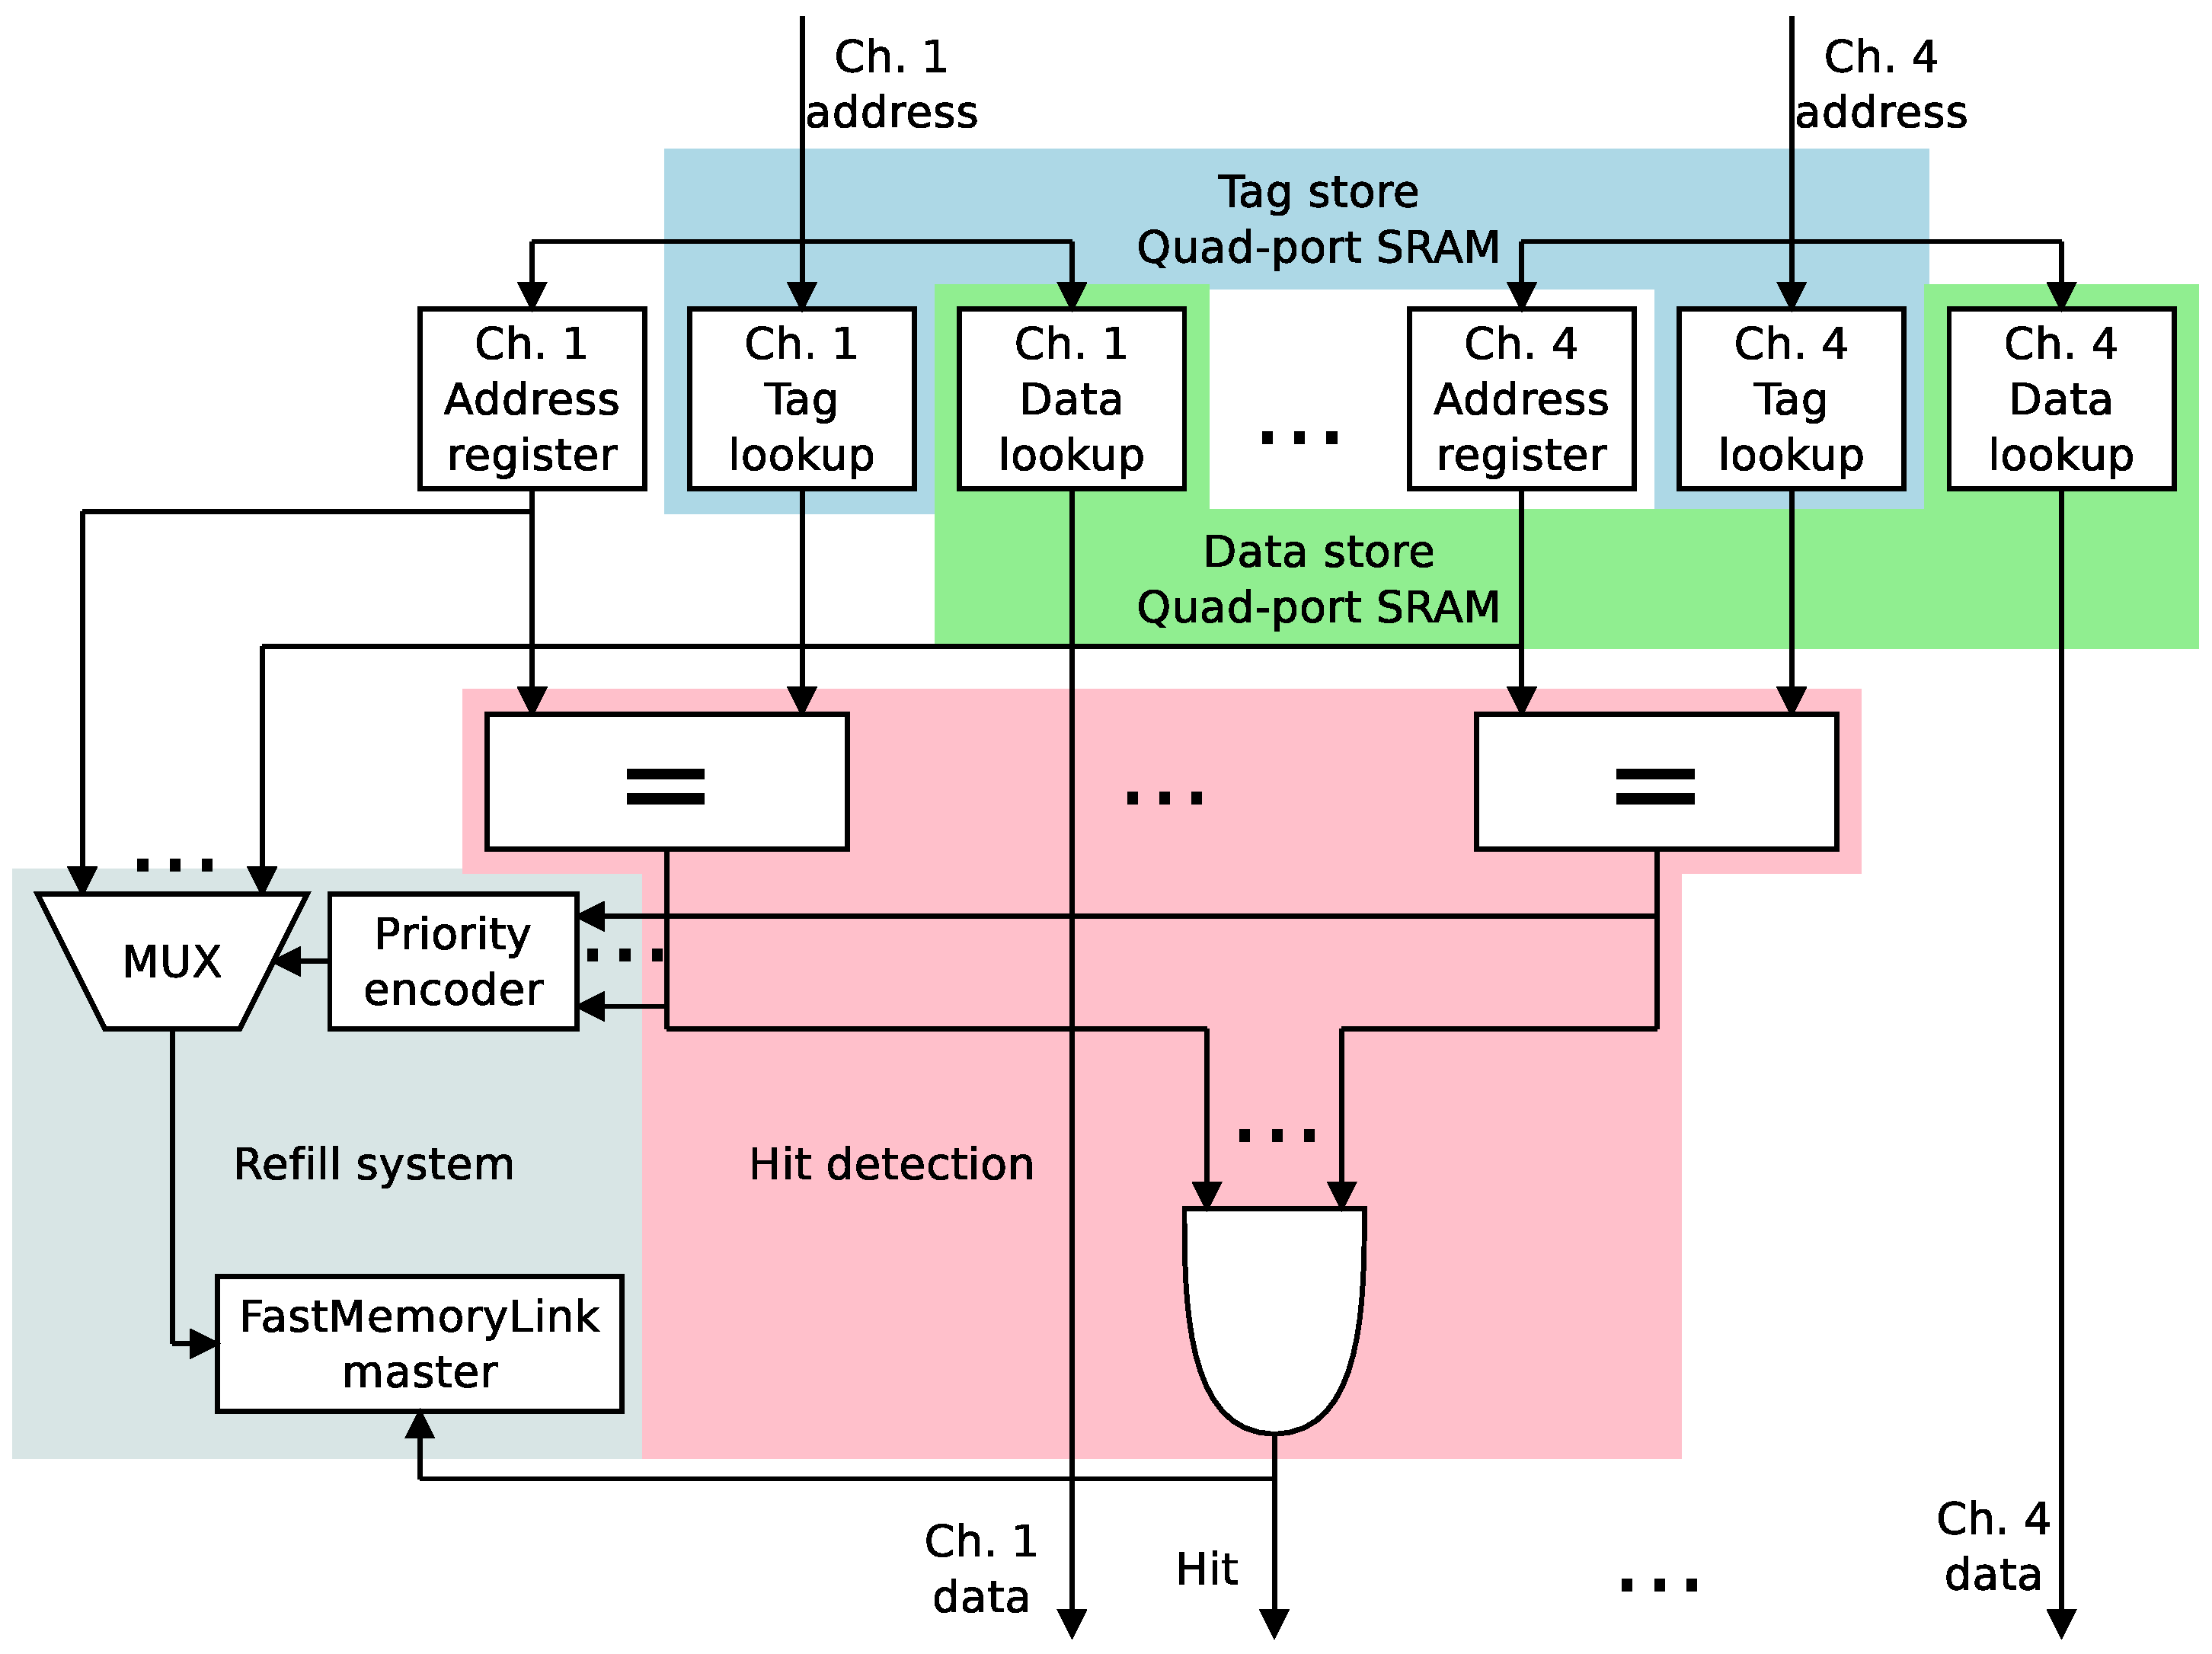
\includegraphics[height=100mm]{tcarch.eps}
\caption{Architecture of the four-channel texel cache.}
\label{fig:tcarch}
\end{figure}

At each clock cycle, the texel cache processes, in a pipelined manner\footnote{The SRAMs are registered, in order to improve timing and to map to the block RAMs of common modern FPGAs which always contain an internal register.}, four memory addresses from each channel if they hit the caches. The ``hit'' signal is kept high and the pipeline is always running.

In case of a miss, the ``hit'' signal goes low (stalling the pipeline), and the priority encoder and the multiplexer (MUX) select one of the missed addresses (there can be one or many). The FastMemoryLink master issues a memory transaction to retrieve the data from the system memory, replaces the contents of the cache line and rewrites the tag. The address now becomes a cache hit. If no other address misses the cache, the texel cache has successfully handled the 4-channel transaction and the ``hit'' signal goes high again to proceed to the next. Otherwise, the process repeats until all addresses hit the cache.

\subsubsection{Inter-channel cache conflicts}
An \textit{inter-channel cache conflict} (ICCC) occurs when two or more channels request different addresses that have different tags but map to the same cache line.

This condition is not desirable. With our implementation, the texel cache would go into an infinite loop fetching data from the memory in an attempt to make all channels hit the cache --- which it can never achieve --- until it is manually reset.\footnote{As a safety measure, it is therefore recommended that software drivers for the texture mapping unit check for the possibility of ICCC conditions before running the TMU and report an error.}

This choice has been made for two reasons: first, adding hardware to deal with ICCCs would yield poor performance anyway as some memory bursts would be there only for retrieving one pixel and solving the conflict\footnote{This is true only if we keep a direct-mapped cache. With a multiple-way set-associative cache and a smart replacement policy that allocates one specific way to each conflicting channel when an ICCC occurs, the hardware can both deal with ICCCs and yield high performance. However, it is more complex and expensive. Furthermore, when keeping a direct-mapped cache, it makes sense to add hardware that would deal with infrequent cases of ICCCs such as those arising when wrapping at texture boundaries.}, second, ICCCs are easy to avoid for our purposes, and we will see how.

For simplicity, we use the pixel (2 bytes) as unit. In the equations that follow:
\begin{itemize}
\item $H$ is the horizontal texture resolution in pixels.
\item $V$ is the vertical texture resolution in pixels.
\item $N_{l}$ is the number of pixels a cache line can hold. It is equal to the line size in bytes divided by 2.
\item $N_{c}$ is the total number of pixels the texel cache can hold. It is equal to the cache size in bytes (not counting the tag memory) divided by 2.
\end{itemize}

\paragraph{Characterization of cache conflicts.} A pixel at address $a_{p}$ (measured in pixels, i.e. 2-byte words) is mapped to the cache line indexed by:
\begin{equation}
l_{p} = \left\lfloor \frac{a_{p}}{N_{l}} \right\rfloor \pmod{\frac{N_{c}}{N_{l}}}
\end{equation}
Thus, two pixels at addresses $a_{1}$ and $a_{2}$ will conflict in the cache if and only if:
\begin{equation}\label{eq:cacheconflict}
\begin{cases}
|a_{1}-a_{2}| \geq N_{l} \\
\left\lfloor \frac{a_{1}}{N_{l}} \right\rfloor \equiv \left\lfloor \frac{a_{2}}{N_{l}} \right\rfloor \pmod{\frac{N_{c}}{N_{l}}}
\end{cases}
\end{equation}

Texture clamping only causes one or more channel addresses to be equal, and therefore does not introduce additional cases of ICCCs. However, texture wrapping does introduce new dispositions of the channels within the texture, and new ICCC conditions.

\paragraph{Conflicts between channels 1 and 2 (or 3 and 4).}
\begin{figure}[htp]
\centering
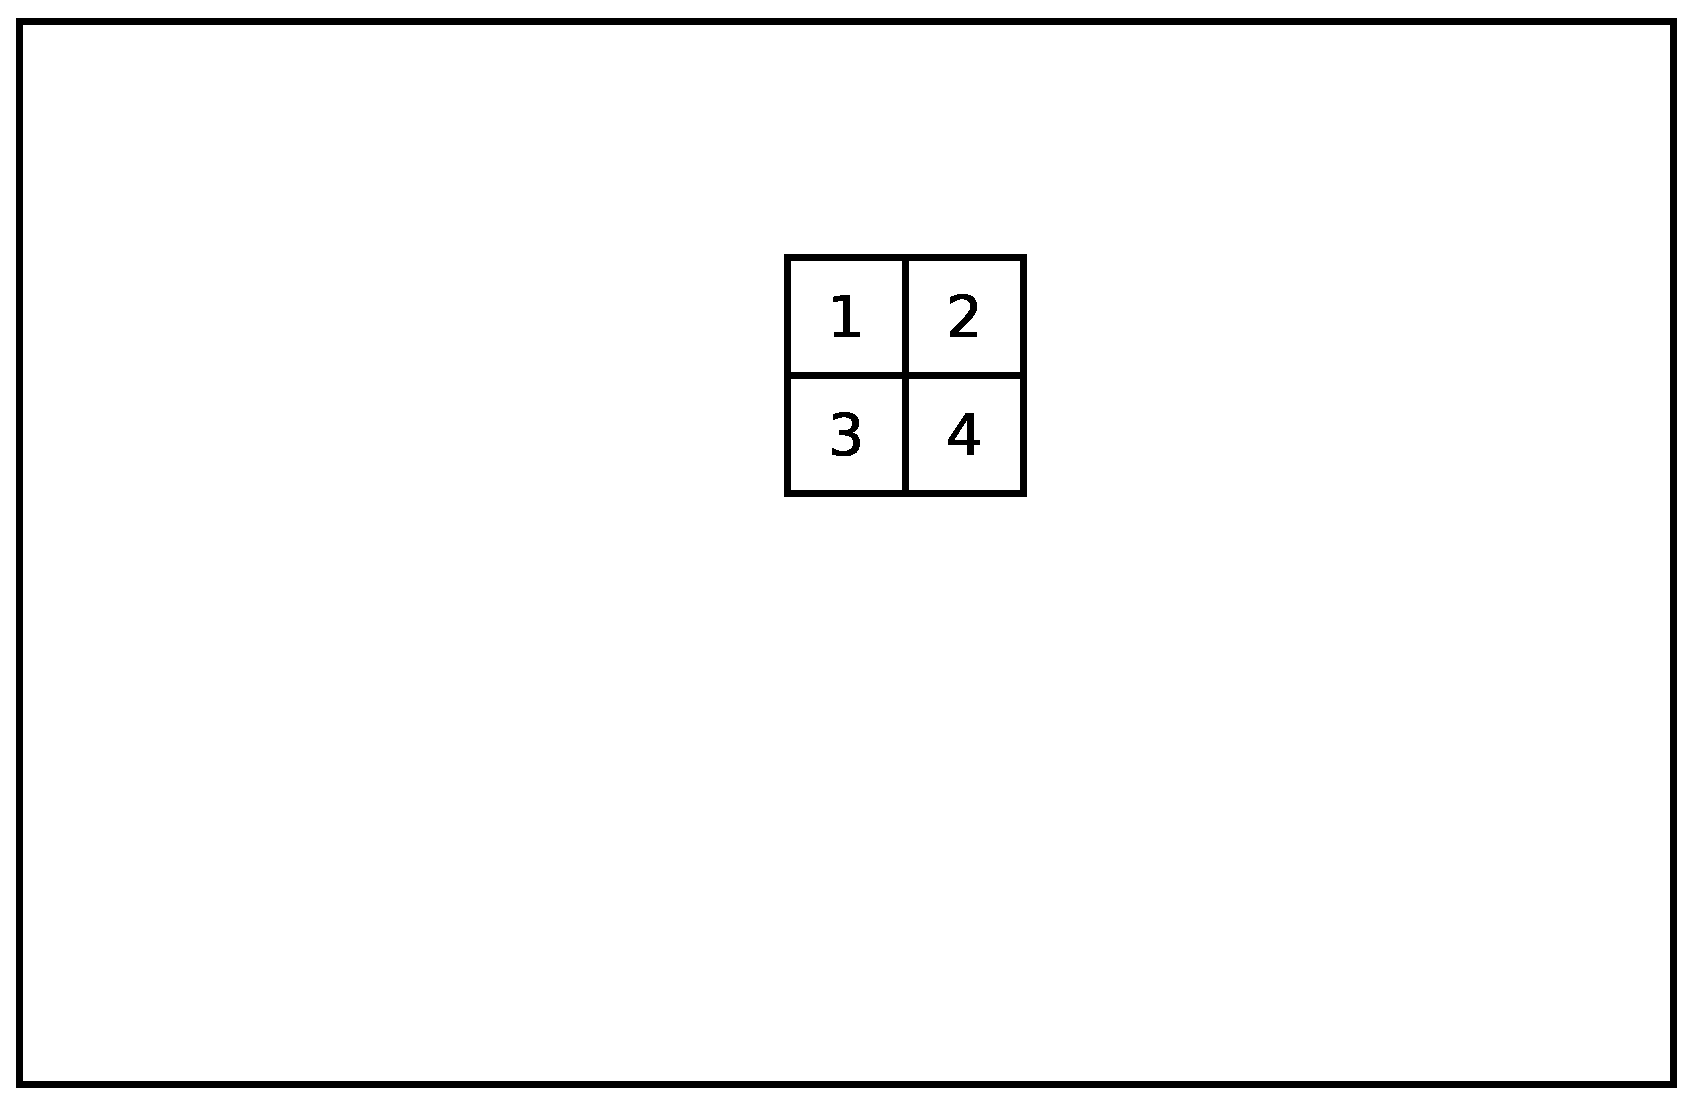
\includegraphics[height=55mm]{chdisp_common.eps}
\caption{Disposition of the channels within the texture, general case.}\label{fig:chdispcommon}
\end{figure}
\begin{figure}[htp]
\centering
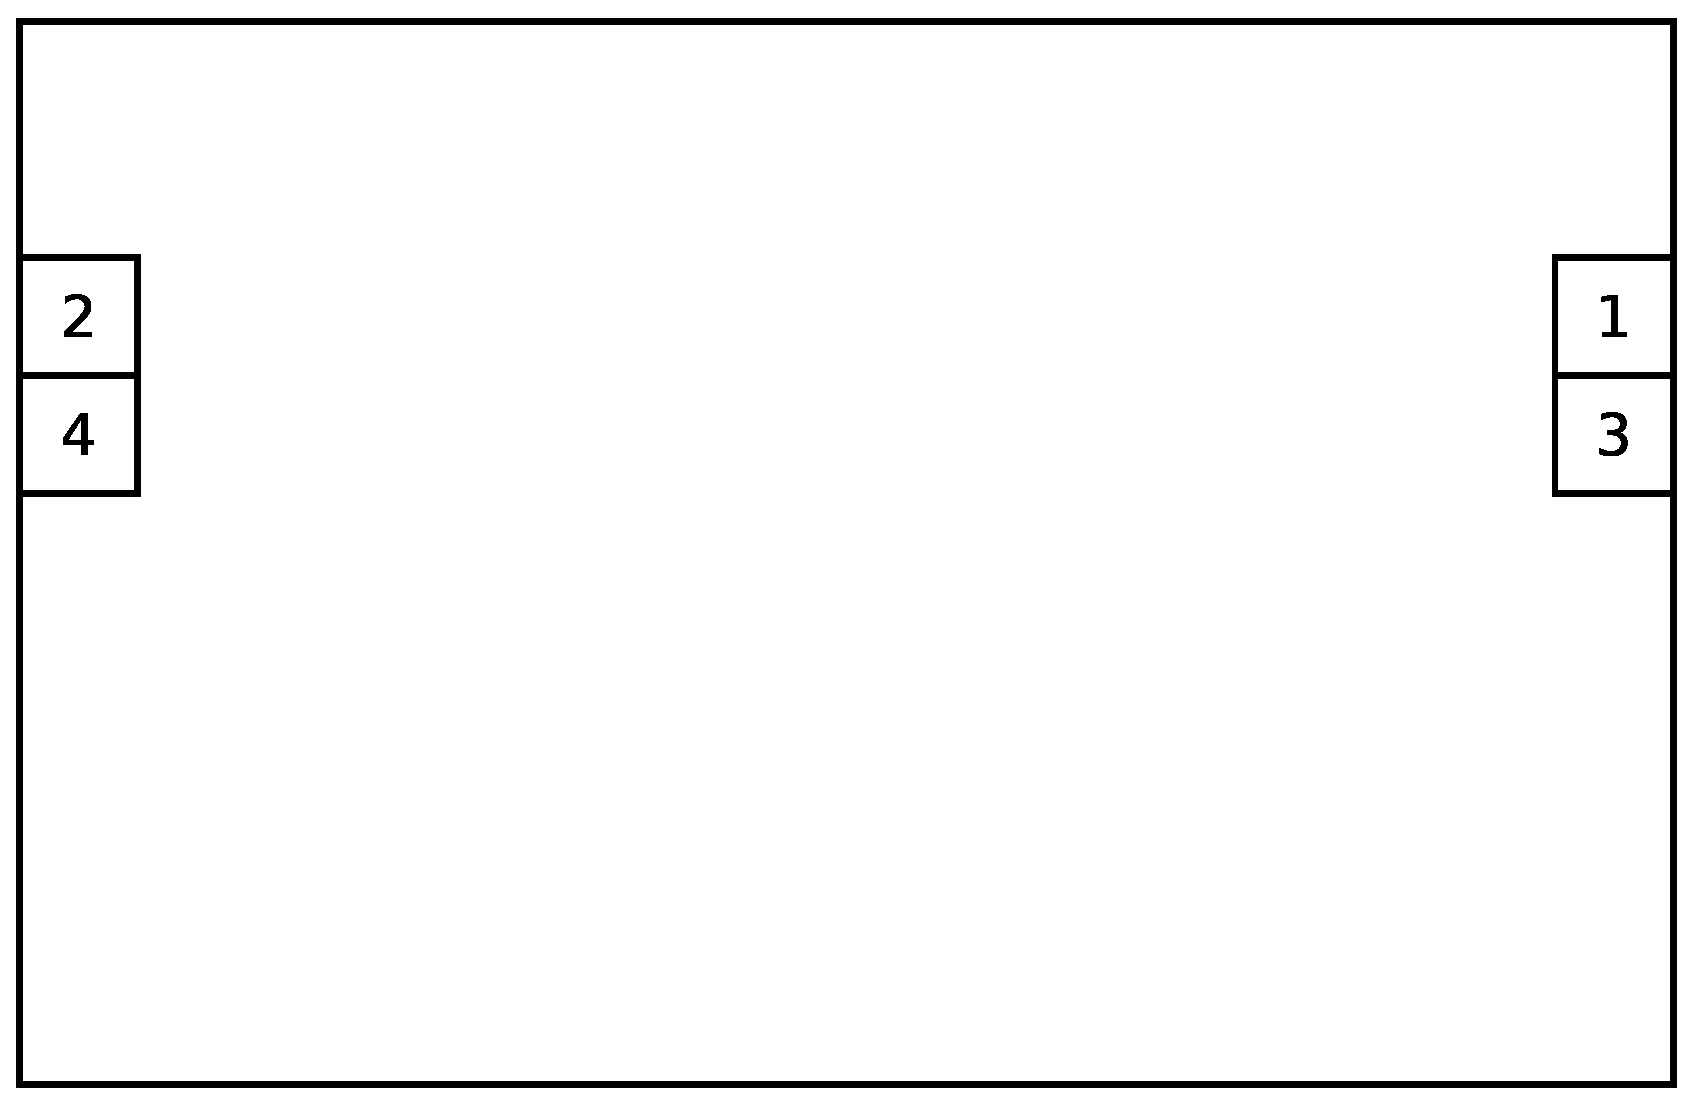
\includegraphics[height=55mm]{chdisp_vwrap.eps}
\caption{Disposition of the channels within the texture, vertical wrapping.}\label{fig:chdispvwrap}
\end{figure}
The addresses $a_{A}$ and $a_{B}$ of these two channels can be separated by either:
\begin{itemize}
\item 1 pixel in the most common case (sampling in the middle of the texture, see figure~\ref{fig:chdispcommon}). This cannot cause inter-channel cache conflicts.
\item $H-1$ pixels if texture wrapping is enabled and the texture is sampled at one of its vertical edges (figure~\ref{fig:chdispvwrap}). In this case, the condition $|a_{A}-a_{B}| \geq N_{l}$ is often verified (except for small textures where $H-1 < N_{l}$). To make sure that there will be no ICCC, we must thus make sure that the following condition is also verified:
\begin{equation}\label{eq:noconflictwrap1}
\left\lfloor \frac{a_{A}}{N_{l}} \right\rfloor \not \equiv \left\lfloor \frac{a_{A}+H-1}{N_{l}} \right\rfloor \pmod{\frac{N_{c}}{N_{l}}}
\end{equation}

To make sure that this condition is verified for all possible pixel addresses, it is sufficient to check that:
\begin{equation}
\forall a \in \{0, 1, ... N_{l}-1\}, \left\lfloor \frac{a+H-1}{N_{l}} \right\rfloor \not \equiv 0 \pmod{\frac{N_{c}}{N_{l}}}
\end{equation}
Indeed, by division by $N_{l}$ we have $a_{A} = k \cdot N_{l} + a$ with $0 \leq a \leq N_{l}-1$, which transforms equation~\ref{eq:noconflictwrap1} into:
\begin{equation}
k + \left\lfloor \frac{a}{N_{l}} \right\rfloor \not \equiv k + \left\lfloor \frac{a+H-1}{N_{l}} \right\rfloor \pmod{\frac{N_{c}}{N_{l}}}
\end{equation}
which leads easily to the result, considering that $\left\lfloor \frac{a}{N_{l}} \right\rfloor = 0$.

This can be further simplified:
\begin{equation}~\label{eq:noconflictwrap2}
\begin{cases}
\left\lfloor \frac{H-1}{N_{l}} \right\rfloor \not \equiv 0 \pmod{\frac{N_{c}}{N_{l}}} \\
1 + \left\lfloor \frac{H-1}{N_{l}} \right\rfloor \not \equiv 0 \pmod{\frac{N_{c}}{N_{l}}}
\end{cases}
\end{equation}
\end{itemize}

\paragraph{Conflicts between channels 1 and 3 (or 2 and 4).}
\begin{figure}[htp]
\centering
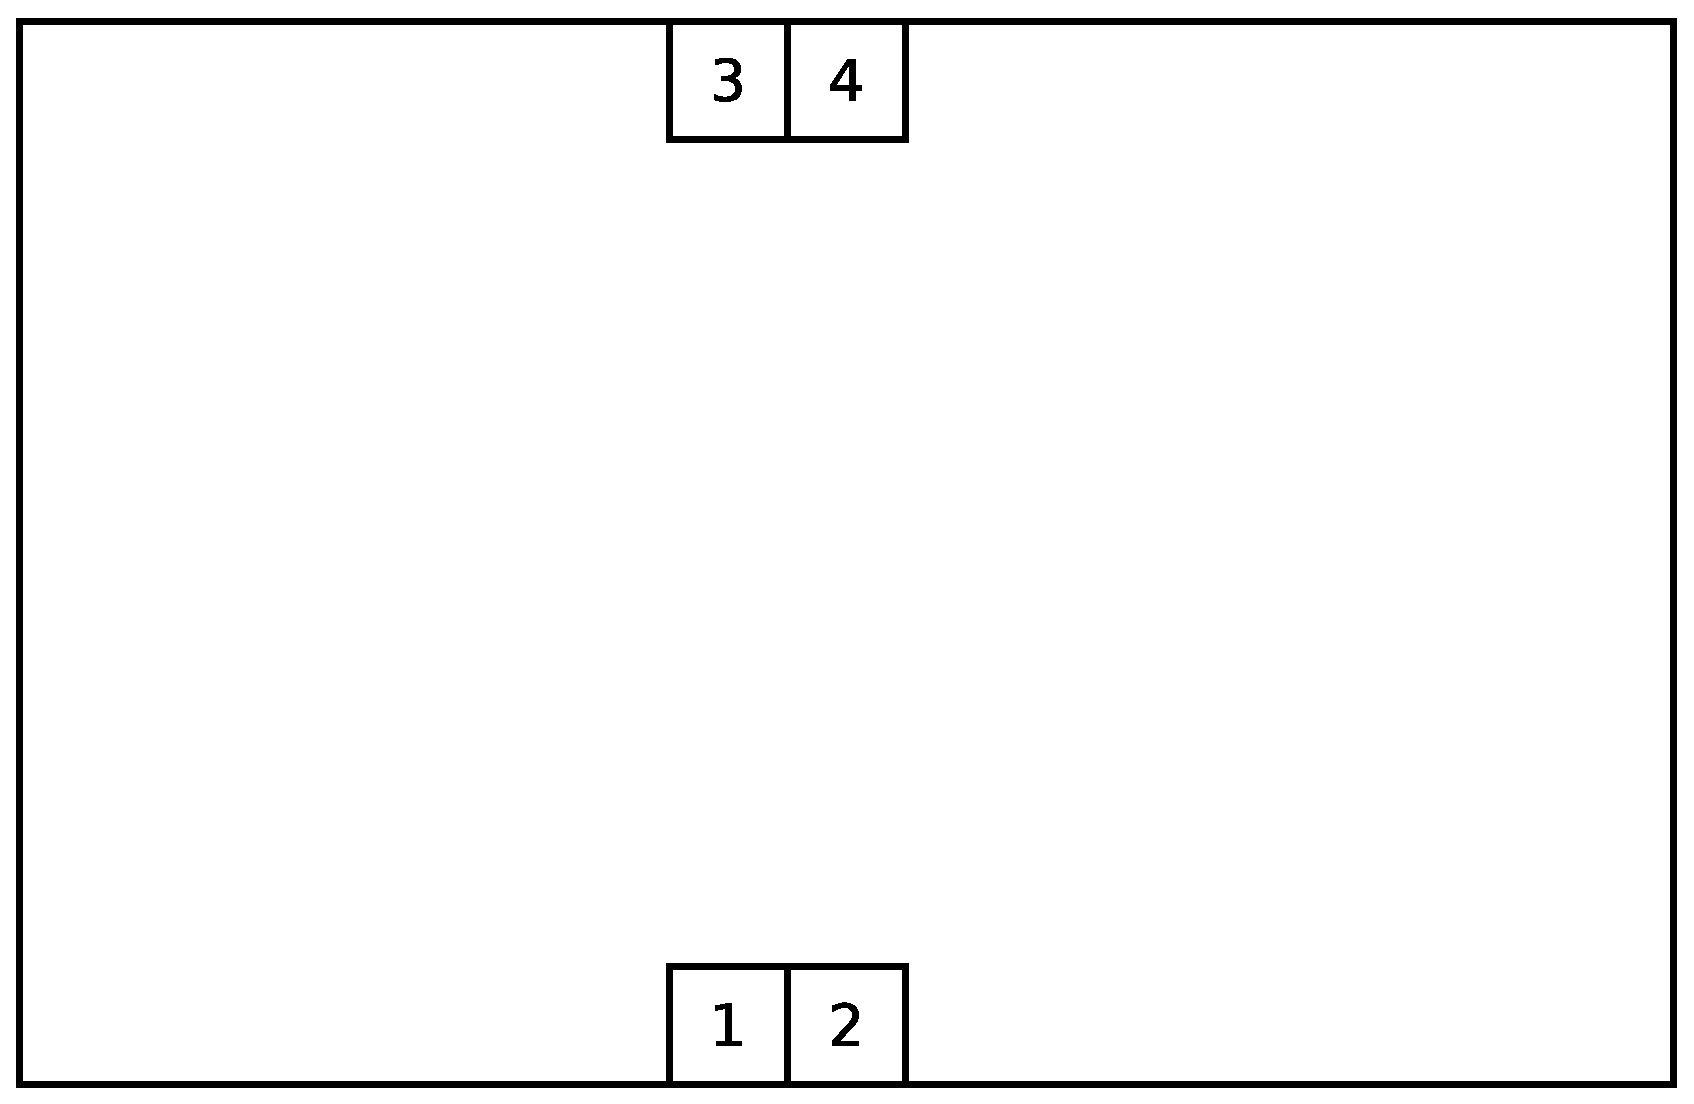
\includegraphics[height=55mm]{chdisp_hwrap.eps}
\caption{Disposition of the channels within the texture, horizontal wrapping.}\label{fig:chdisphwrap}
\end{figure}
The separation between the channels' addresses can be:
\begin{itemize}
\item $H$ pixels (according to equation~\ref{eq:fbadr}) in the general case (figure~\ref{fig:chdispcommon}). Using the same reasoning from above, we can deduce that it is sufficient to check that $H < N_{l}$ or:
\begin{equation}
\begin{cases}
\left\lfloor \frac{H}{N_{l}} \right\rfloor \not \equiv 0 \pmod{\frac{N_{c}}{N_{l}}} \\
1 + \left\lfloor \frac{H}{N_{l}} \right\rfloor \not \equiv 0 \pmod{\frac{N_{c}}{N_{l}}}
\end{cases}
\end{equation}
\item $H \cdot (V-1)$ pixels if texture wrapping is enabled and the texture is sampled at one of its horizontal edges (figure~\ref{fig:chdisphwrap}). Again, it is sufficient to check that $H \cdot (V-1) < N_{l}$ or:
\begin{equation}
\begin{cases}
\left\lfloor \frac{H \cdot (V-1)}{N_{l}} \right\rfloor \not \equiv 0 \pmod{\frac{N_{c}}{N_{l}}} \\
1 + \left\lfloor \frac{H \cdot (V-1)}{N_{l}} \right\rfloor \not \equiv 0 \pmod{\frac{N_{c}}{N_{l}}}
\end{cases}
\end{equation}
\end{itemize}

\paragraph{Conflicts between channels 1 and 4.}
\begin{figure}[htp]
\centering
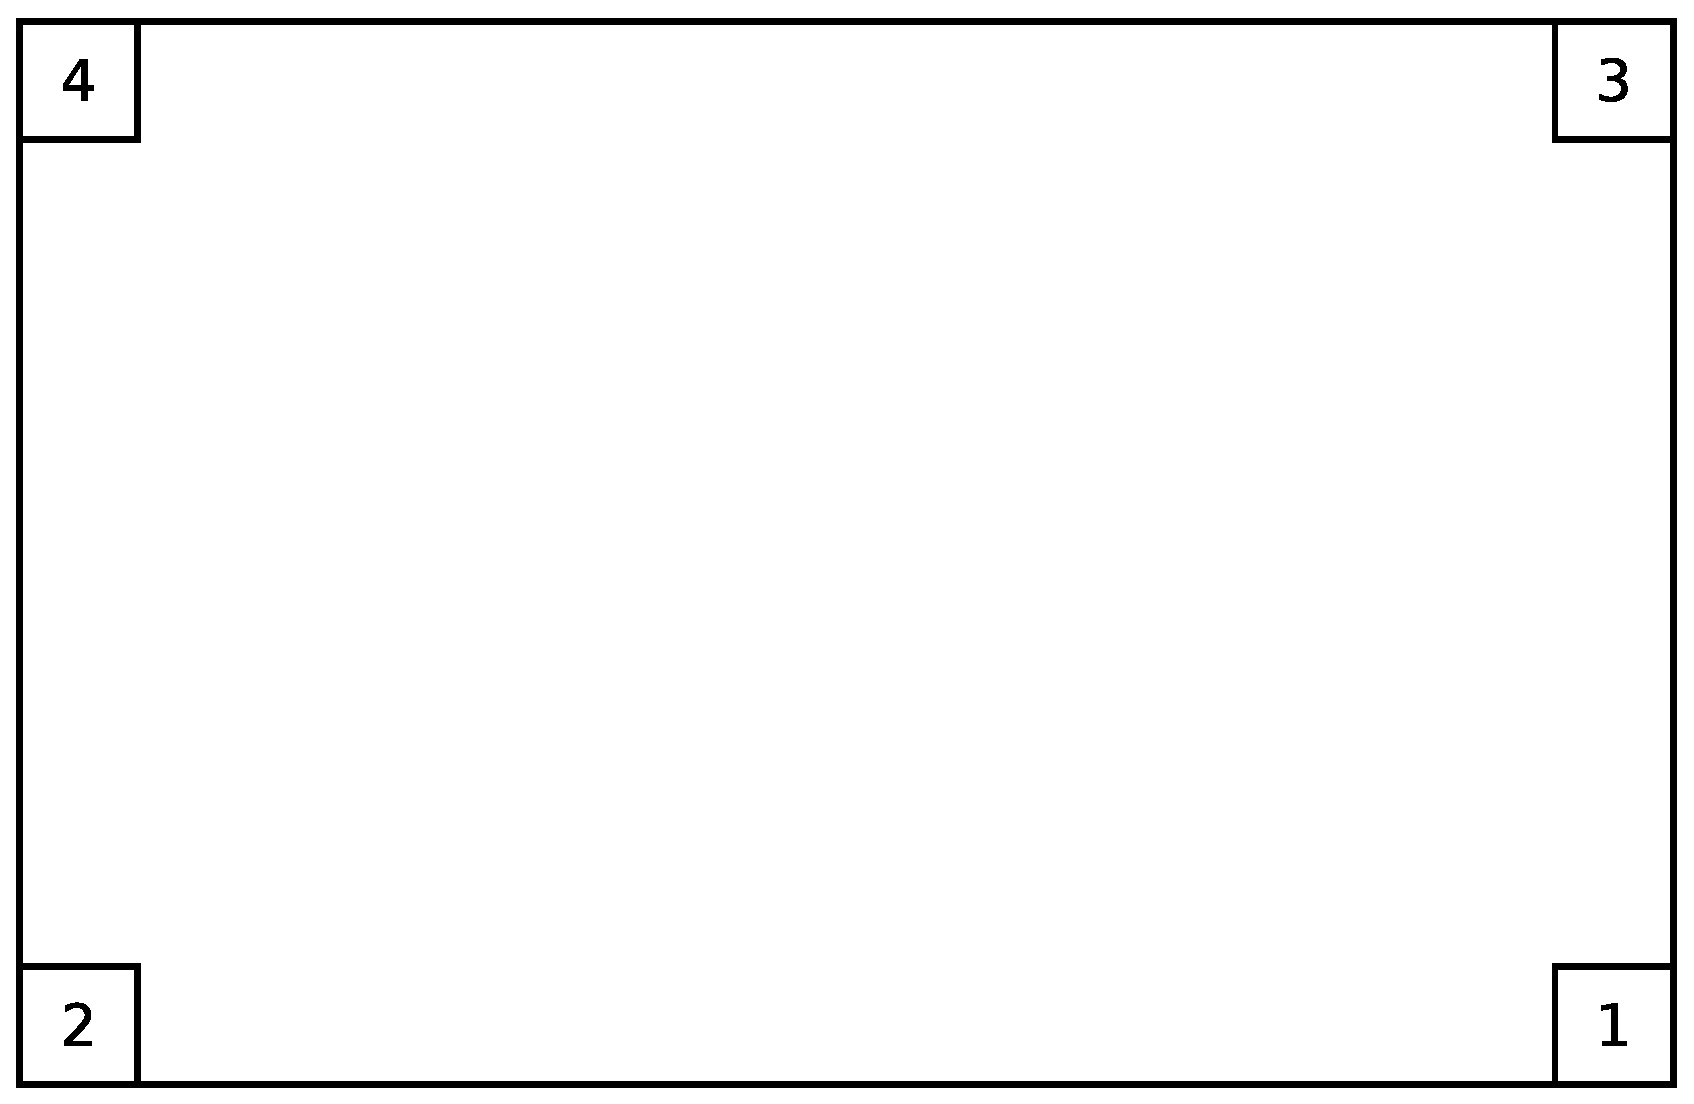
\includegraphics[height=55mm]{chdisp_hvwrap.eps}
\caption{Disposition of the channels within the texture, horizontal and vertical wrapping.}\label{fig:chdisphvwrap}
\end{figure}
The channels' addresses can be separated by:
\begin{itemize}
\item $H + 1$ pixels (according to equation~\ref{eq:fbadr}) in the general case (figure~\ref{fig:chdispcommon}). It is therefore sufficient to check that $H+1 < N_{l}$ or:
\begin{equation}
\begin{cases}
\left\lfloor \frac{H+1}{N_{l}} \right\rfloor \not \equiv 0 \pmod{\frac{N_{c}}{N_{l}}} \\
1 + \left\lfloor \frac{H+1}{N_{l}} \right\rfloor \not \equiv 0 \pmod{\frac{N_{c}}{N_{l}}}
\end{cases}
\end{equation}
\item 1 pixel in case of vertical wrapping (figure~\ref{fig:chdispvwrap}). This cannot cause ICCCs.
\item $H \cdot (V-1) - 1$ pixels in case of horizontal wrapping (figure~\ref{fig:chdisphwrap}). Similarly, we can check that $H \cdot (V-1) - 1 < N_{l}$ or:
\begin{equation}
\begin{cases}
\left\lfloor \frac{H \cdot (V-1) - 1}{N_{l}} \right\rfloor \not \equiv 0 \pmod{\frac{N_{c}}{N_{l}}} \\
1 + \left\lfloor \frac{H \cdot (V-1) - 1}{N_{l}} \right\rfloor \not \equiv 0 \pmod{\frac{N_{c}}{N_{l}}}
\end{cases}
\end{equation}
\item $H \cdot V - 1$ in case of wrapping in both directions (figure~\ref{fig:chdisphvwrap}). We can check that $H \cdot V - 1 < N_{l}$ or:
\begin{equation}
\begin{cases}
\left\lfloor \frac{H \cdot V - 1}{N_{l}} \right\rfloor \not \equiv 0 \pmod{\frac{N_{c}}{N_{l}}} \\
1 + \left\lfloor \frac{H \cdot V - 1}{N_{l}} \right\rfloor \not \equiv 0 \pmod{\frac{N_{c}}{N_{l}}}
\end{cases}
\end{equation}
\end{itemize}

\paragraph{Conflicts between channels 2 and 3.}
Like above, we can check that $H-1 < N_{l}$ or:
\begin{equation}~\label{eq:noconflictwrap2}
\begin{cases}
\left\lfloor \frac{H-1}{N_{l}} \right\rfloor \not \equiv 0 \pmod{\frac{N_{c}}{N_{l}}} \\
1 + \left\lfloor \frac{H-1}{N_{l}} \right\rfloor \not \equiv 0 \pmod{\frac{N_{c}}{N_{l}}}
\end{cases}
\end{equation}

Furthermore, if texture wrapping is enabled, the differences between pixel addresses can become (resulting in similar conditions to check for):
\begin{itemize}
\item $2 \cdot H - 1$ (vertical wrapping, figure~\ref{fig:chdispvwrap}).
\item $H \cdot (V - 1) + 1$ (horizontal wrapping, figure~\ref{fig:chdisphwrap}).
\item $H \cdot (V - 2) + 1$ (wrapping in both directions, figure~\ref{fig:chdisphvwrap}).
\end{itemize}

\paragraph{Summary.}
To avoid inter-channel cache conflicts, when texture clamping is used, it is sufficient to check that (all equivalences are modulo $\frac{N_{c}}{N_{l}}$):
\begin{equation}
\boxed{
\begin{cases}
H-1 < N_{l} & \textrm{ or } \begin{cases}
\left\lfloor \frac{H-1}{N_{l}} \right\rfloor \not \equiv 0 \\
1 + \left\lfloor \frac{H-1}{N_{l}} \right\rfloor \not \equiv 0
\end{cases} \\
H < N_{l} & \textrm{ or } \begin{cases}
\left\lfloor \frac{H}{N_{l}} \right\rfloor \not \equiv 0 \\
1 + \left\lfloor \frac{H}{N_{l}} \right\rfloor \not \equiv 0
\end{cases} \\
H+1 < N_{l} & \textrm{ or } \begin{cases}
\left\lfloor \frac{H+1}{N_{l}} \right\rfloor \not \equiv 0 \\
1 + \left\lfloor \frac{H+1}{N_{l}} \right\rfloor \not \equiv 0
\end{cases}
\end{cases}
}
\end{equation}

If texture wrapping is used, additional conditions appear:
\begin{equation}
\boxed{
\begin{cases}
H \cdot (V-1) - 1 < N_{l} & \textrm{ or } \begin{cases}
\left\lfloor \frac{H \cdot (V-1) - 1}{N_{l}} \right\rfloor \not \equiv 0 \\
1 + \left\lfloor \frac{H \cdot (V-1) - 1}{N_{l}} \right\rfloor \not \equiv 0
\end{cases} \\
H \cdot (V-1) < N_{l} & \textrm{ or } \begin{cases}
\left\lfloor \frac{H \cdot (V-1)}{N_{l}} \right\rfloor \not \equiv 0 \\
1 + \left\lfloor \frac{H \cdot (V-1)}{N_{l}} \right\rfloor \not \equiv 0
\end{cases} \\
H \cdot (V-1) + 1 < N_{l} & \textrm{ or } \begin{cases}
\left\lfloor \frac{H \cdot (V-1) + 1}{N_{l}} \right\rfloor \not \equiv 0 \\
1 + \left\lfloor \frac{H \cdot (V-1) + 1}{N_{l}} \right\rfloor \not \equiv 0
\end{cases} \\
H \cdot (V-2) + 1 < N_{l} & \textrm{ or } \begin{cases}
\left\lfloor \frac{H \cdot (V-2) + 1}{N_{l}} \right\rfloor \not \equiv 0 \\
1 + \left\lfloor \frac{H \cdot (V-2) + 1}{N_{l}} \right\rfloor \not \equiv 0
\end{cases} \\
2 \cdot H - 1 < N_{l} & \textrm{ or } \begin{cases}
\left\lfloor \frac{2 \cdot H - 1}{N_{l}} \right\rfloor \not \equiv 0 \\
1 + \left\lfloor \frac{2 \cdot H - 1}{N_{l}} \right\rfloor \not \equiv 0
\end{cases} \\
H \cdot V - 1 < N_{l} & \textrm{ or } \begin{cases}
\left\lfloor \frac{H \cdot V - 1}{N_{l}} \right\rfloor \not \equiv 0 \\
1 + \left\lfloor \frac{H \cdot V - 1}{N_{l}} \right\rfloor \not \equiv 0
\end{cases}
\end{cases}
}
\end{equation}

\subsubsection{Cache size}
We must now determine an optimal size for the texel cache. The size must represent a compromise between hit rate (and, thus, performance) and costly utilization of on-chip RAM. Furthermore, it must be chosen so that inter-channel cache conflicts do not occur for our use cases.

To study the impact of the cache size on the hit rate, we simulated the complete Verilog code of texture mapping unit with different cache sizes. The CSR interface of the texture mapping unit (subsection~\ref{subsec:tmucsr}) supports eight registers that measure, for each channel, the number of requests\footnote{As outlined above, channels are only active (i.e. issue a cache request) when needed (i.e. when the interpolated texture coordinates are not integer). Channel 1 is always active and therefore makes as many accesses as there are pixels in the output picture. Its accesses are however still counted as a means to check that the texture mapping unit is operating correctly.} and how many of those requests hit the cache. Those registers are still present after logic synthesis, and can be used to validate the performance of the texel cache in the real system.\footnote{The reason why we performed the tests using Verilog simulations instead of the real FPGA-based system is because logic synthesis --- needed for each tested cache size --- takes a long time, and some cache configurations may cause resource shortages or timing problems that would need to be manually addressed.}

The source and destination images have a resolution of 512x512 pixels, and are tesselated with 16x16 rectangles forming a 32x32 mesh --- which matches the configuration used for distortions by the renderer program. Different sets of texture coordinates were used at each vertex, according to table~\ref{tab:tcsets}. Texture coordinates are multiplied by 64 to perform the conversion of integers into the fixed point format used throughout the linear interpolation process (see subsection~\ref{subsec:bilfpformat}). $x$ and $y$ refer to the indices of the vertex in the mesh. Texture wrapping was enabled, as it puts more load on the cache than texture clamping.

The sets were chosen for the following reasons:
\begin{itemize}
\item \textit{copy} does not introduce any distortion and is meant to test the performance of the TMU as a blitter, that could be used e.g. for GUI acceleration. It is also a very simple case that verifies the consistency of the results.
\item \textit{zoomin} scales up the picture. This tests the TMU in a favorable case: as the amount of zoom is important, the texels are swept across slower than output pixels are drawn. This is expected to generate a lot of cache hits.
\item \textit{zoomout} scales down and repeats the picture. This is a detrimental case: the texels are swept across faster than the output pixel are drawn, and some values from the cache lines read from memory will have to be discarded. This is expected to generate a lot of cache misses.
\item \textit{rotozoom} slightly scales down and rotates the picture. This is an intermediate case that reflects what MilkDrop typically does: rotation and slight scale-down are common preset effects.
\end{itemize}

\begin{table}
\centering
\begin{tabularx}{13cm}{|c|c|X|X|}
\hline
\textbf{Set name} & \textbf{Output picture} & \textbf{X} & \textbf{Y} \\
\hline
copy & Figure~\ref{fig:tmuoutcopy} & $x \cdot 16 \cdot 64$ & $y \cdot 16 \cdot 64$ \\
\hline
zoomin & Figure~\ref{fig:tmuoutzoomin} & $x \cdot 10 \cdot 64$ & $y \cdot 10 \cdot 64$ \\
\hline
zoomout & Figure~\ref{fig:tmuoutzoomout} & $x \cdot 40 \cdot 64$ & $y \cdot 40 \cdot 64$ \\
\hline
rotozoom & Figure~\ref{fig:tmuoutrotozoom} & $(x\cdot16-256)\cdot67 - (y\cdot16-256)\cdot28+256\cdot64$ & $(x\cdot16-256)\cdot28 + (y\cdot16-256)\cdot67+256\cdot64$ \\
\hline
\end{tabularx}
\caption{Texture coordinate sets used for benchmarking the texel cache.}\label{tab:tcsets}
\end{table}

\begin{figure}[htp]
\centering
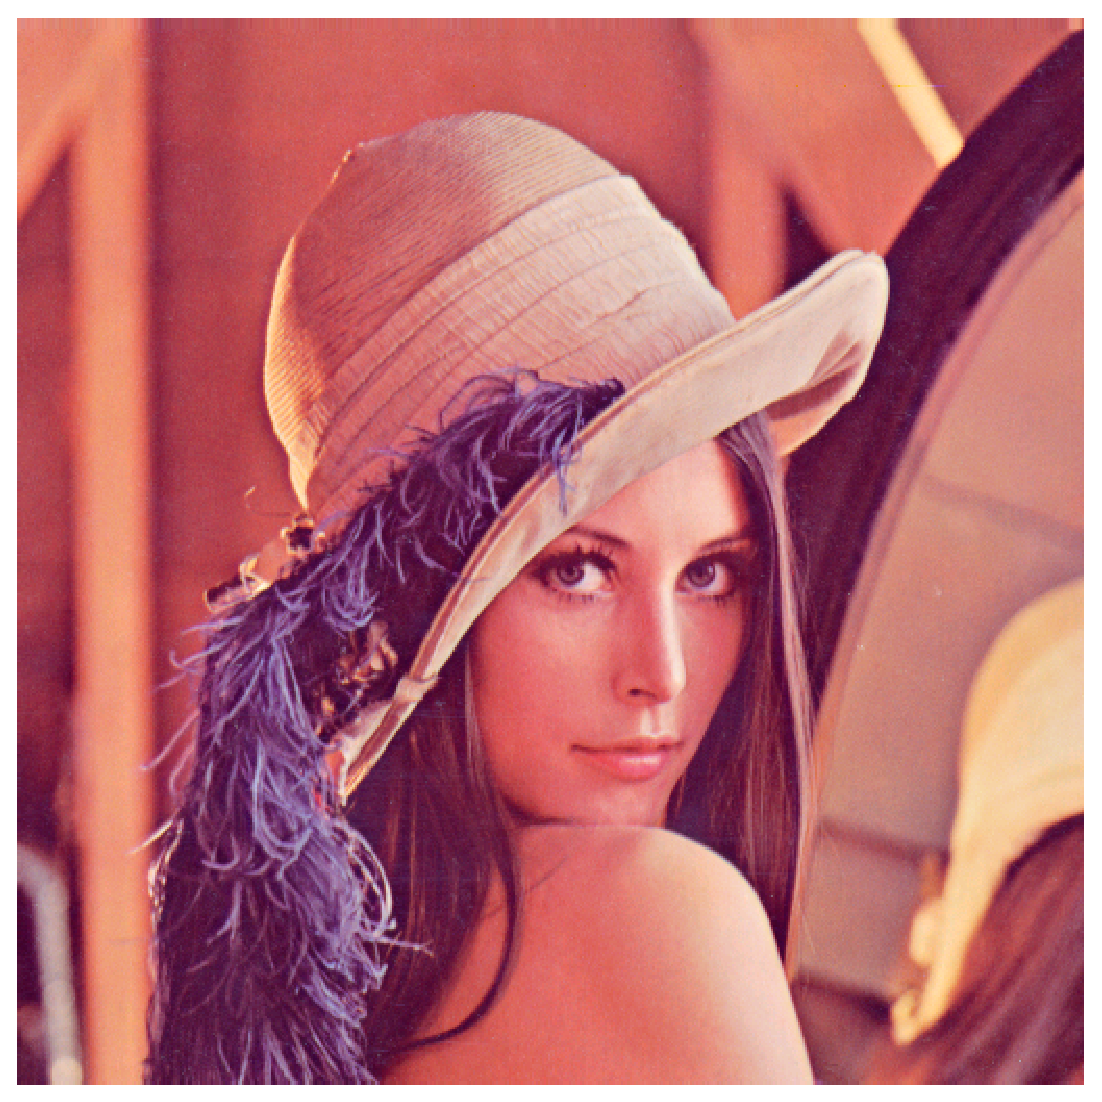
\includegraphics[height=85mm]{tmuout_copy.eps}
\caption{TMU output picture for the ``copy'' set (original picture).}
\label{fig:tmuoutcopy}
\end{figure}

\begin{figure}[htp]
\centering
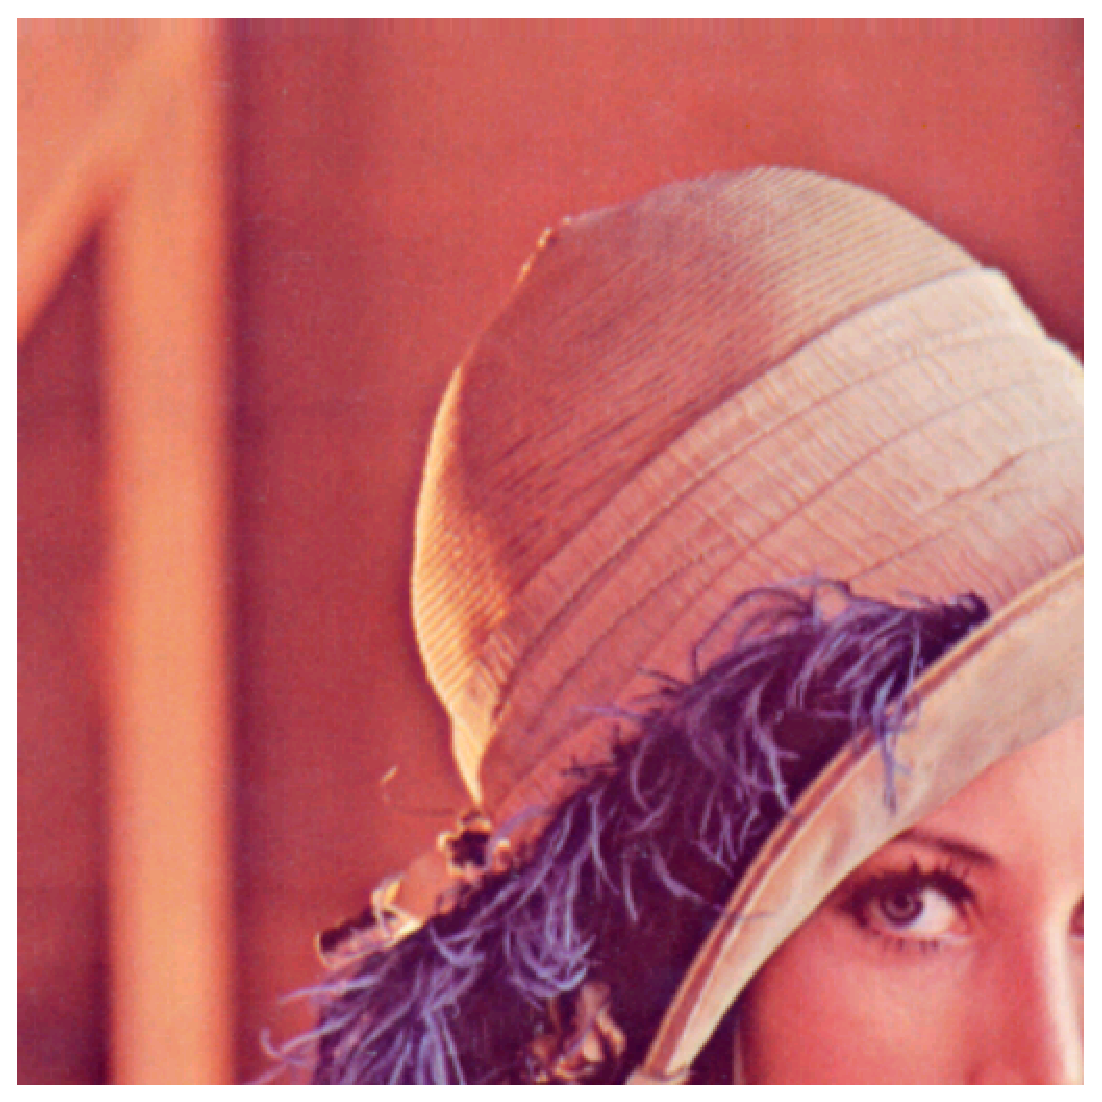
\includegraphics[height=85mm]{tmuout_zoomin.eps}
\caption{TMU output picture for the ``zoomin'' set.}
\label{fig:tmuoutzoomin}
\end{figure}

\begin{figure}[htp]
\centering
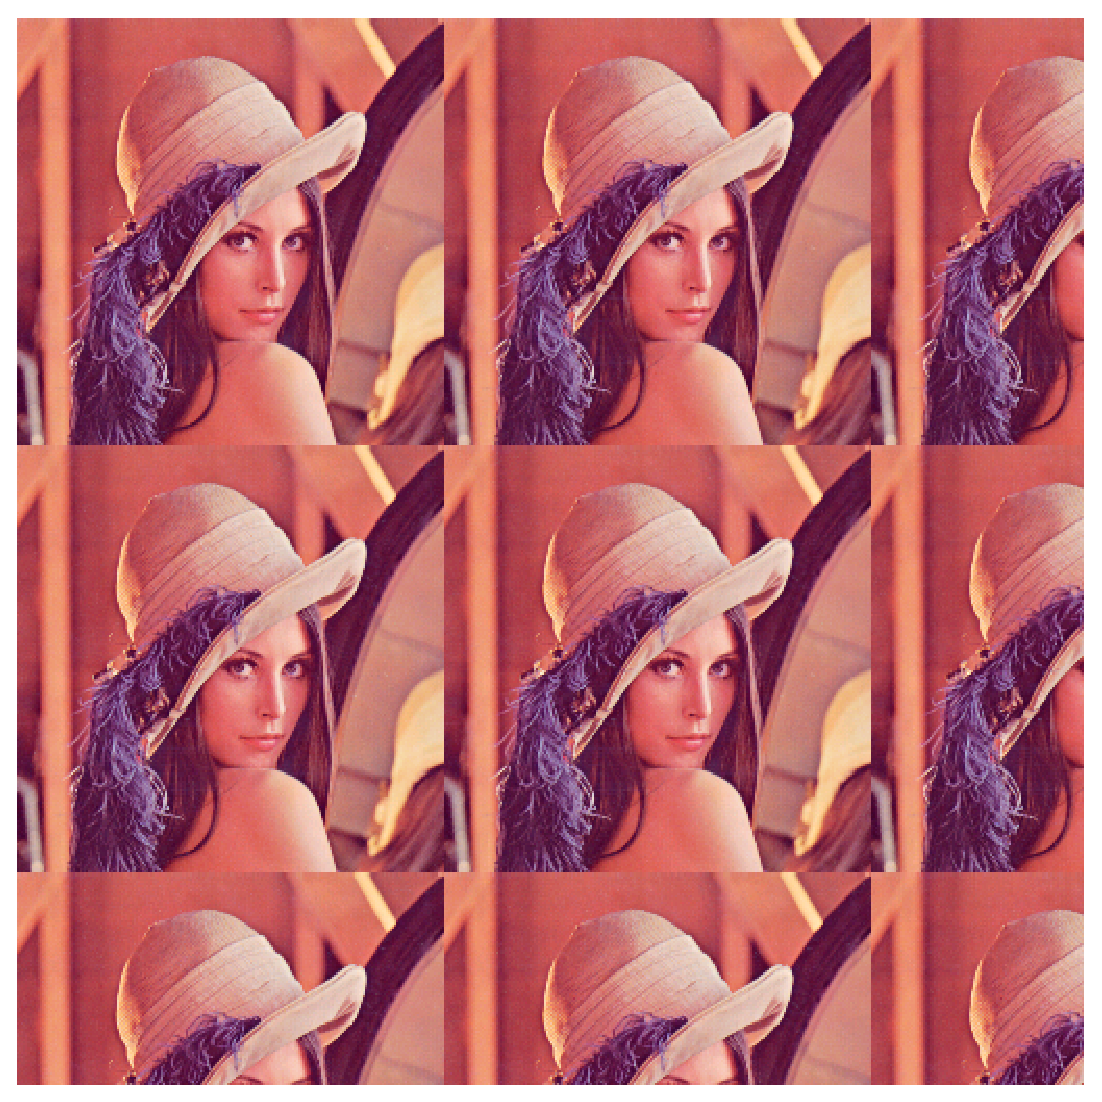
\includegraphics[height=85mm]{tmuout_zoomout.eps}
\caption{TMU output picture for the ``zoomout'' set.}
\label{fig:tmuoutzoomout}
\end{figure}

\begin{figure}[htp]
\centering
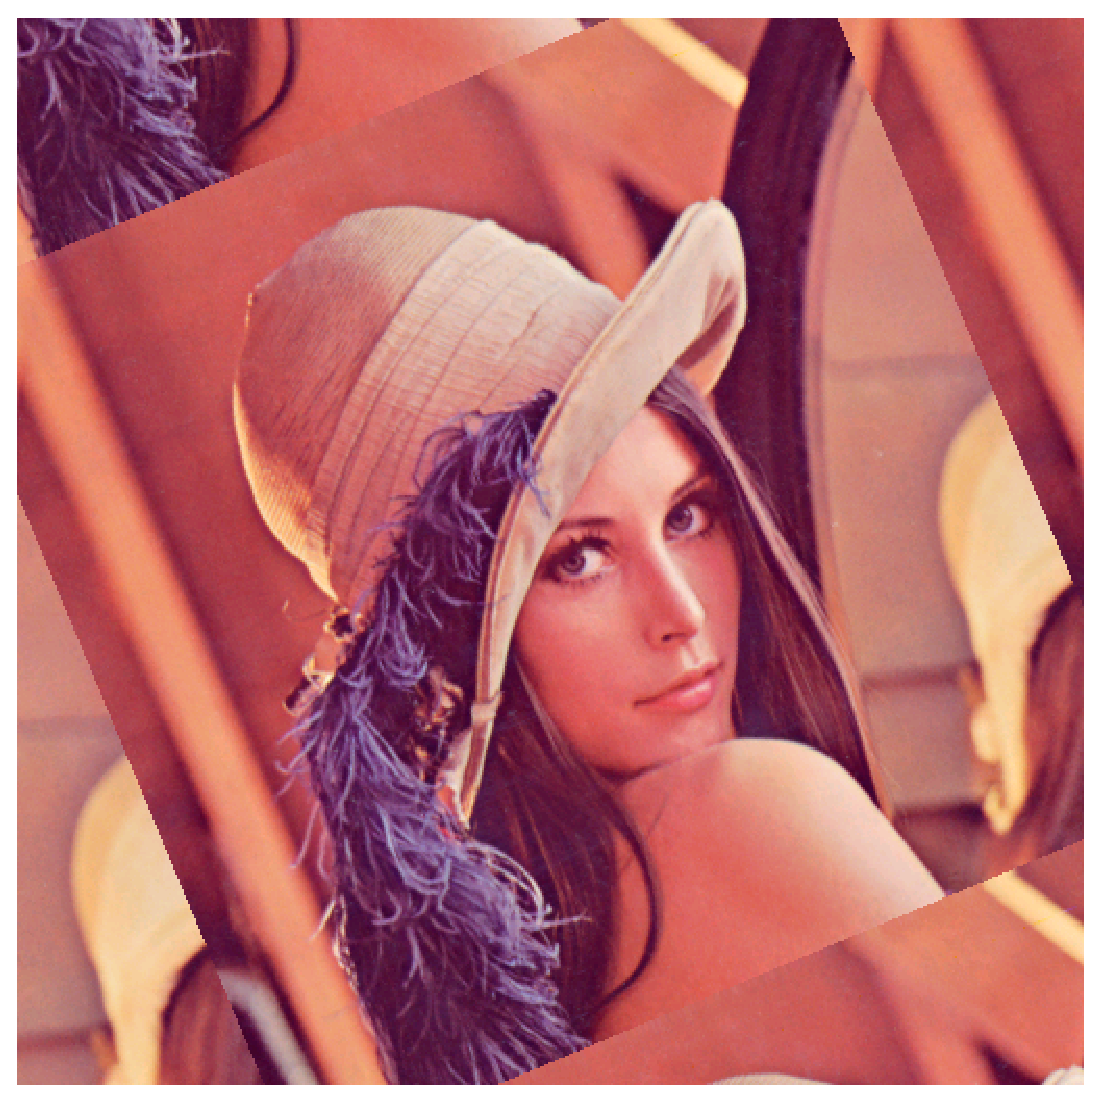
\includegraphics[height=85mm]{tmuout_rotozoom.eps}
\caption{TMU output picture for the ``rotozoom'' set.}
\label{fig:tmuoutrotozoom}
\end{figure}

The length of the cache line is set to the length of a FML burst in the SoC (4 words of 64 bits each) for simplicity of the design.

Simulations were carried out using the free GPL Cver Verilog simulator~\cite{gplcver}. To visually inspect the results of the distortions stemming from each set of texture coordinates, the simulation reads and writes input and output picture files thanks to a Verilog VPI~\cite{vpi} plug-in.\footnote{This was also part of the usual test bench used to debug the Verilog implementation of the texture mapping unit.} A typical simulation trace is reproduced in figure~\ref{fig:tmusimtrace}. Even though GPL Cver is relatively slow\footnote{Its runtime is between one and three minutes on a Intel Core 2 Duo 2.5GHz machine.} to carry out such a complex simulation, it produced consistent results, which supports the idea that it is a viable alternative to proprietary and expensive simulators commonly taught in university courses.

\begin{figure}
\centering
\begin{boxedminipage}{13cm}
\begin{verbatim}
$ make TB=tb_tmu2.v
cver +loadvpi=./vpi_images.so:vpi_register tb_tmu2.v
(...)
GPLCVER_2.12a of 05/16/07 (Linux-elf).
Copyright (c) 1991-2007 Pragmatic C Software Corp.
  All Rights reserved.  Licensed under the GNU General Public
  License (GPL).
  See the 'COPYING' file for details.  NO WARRANTY provided.
Today is Tue May  4 14:46:22 2010.
PLI Image I/O functions registered
Compiling source file "tb_tmu2.v"
Compiling source file "../rtl/tmu2_adrgen.v"
(...)

Opening input picture...
Configuring TMU...
CSR write: 0000002c=01000000
CSR write: 00000004=00000020
(...)
CSR write: 00000044=00000010
CSR write: 00000048=0000003f
Starting TMU...
CSR write: 00000000=00000001
Received DONE IRQ from TMU!
Gathering texel cache statistics...
CSR read : 00000050=00040000
CSR read : 00000054=0003c000
(...)
CSR read : 00000068=00000000
CSR read : 0000006c=00000000
Channel A:      245760 /      262144 hits (93.750000 %)
Channel B:           0 /           0 hits (nan %)
Channel C:           0 /           0 hits (nan %)
Channel D:           0 /           0 hits (nan %)
GLOBAL   :      245760 /      262144 hits (93.750000 %)
Writing output picture...
All done!
Halted at location **tb_tmu2.v(367) time 4585546 from call
to $finish.
  There were 0 error(s), 32 warning(s), and 402 inform(s).
\end{verbatim}
\end{boxedminipage}
\caption{Typical TMU simulation trace (excerpt).}
\label{fig:tmusimtrace}
\end{figure}

Results are reported in table~\ref{tab:tcresults} and figure~\ref{fig:tcresultsgraph}. Only the \textit{global} hit rate is reported, which is computed as the global number of hits over the global number of accesses. The global number of hits (respectively  accesses) is the sum of the number of hits (respectively accesses) for all channels. The reported cache size is the size of the data store only (not counting the tag memory).

\begin{table}
\centering
\begin{tabular}{|c|c|c|c|c|}
\hline
\textbf{Cache size} & \textbf{copy} & \textbf{zoomin} & \textbf{zoomout} & \textbf{rotozoom} \\
\hline
2KB & 93.75 \% & 98.08 \% & 83.33 \% & 73.06 \% \\
\hline
4KB & 93.75 \% & 98.08 \% & 83.33 \% & 82.94 \% \\
\hline
8KB & 93.75 \% & 98.62 \% & 83.33 \% & 93.73 \% \\
\hline
16KB & 93.75 \% & 99.27 \% & 86.94 \% & 95.74 \% \\
\hline
32KB & 93.75 \% & 99.27 \% & 91.44 \% & 96.02 \% \\
\hline
64KB & 93.75 \% & 99.27 \% & 94.14 \% & 96.02 \% \\
\hline
128KB & 93.75 \% & 99.27 \% & 94.14 \% & 96.15 \% \\
\hline
\end{tabular}
\caption{Hit rates for each set of texture coordinates and different cache sizes.}\label{tab:tcresults}
\end{table}

\begin{figure}[htp]
\centering
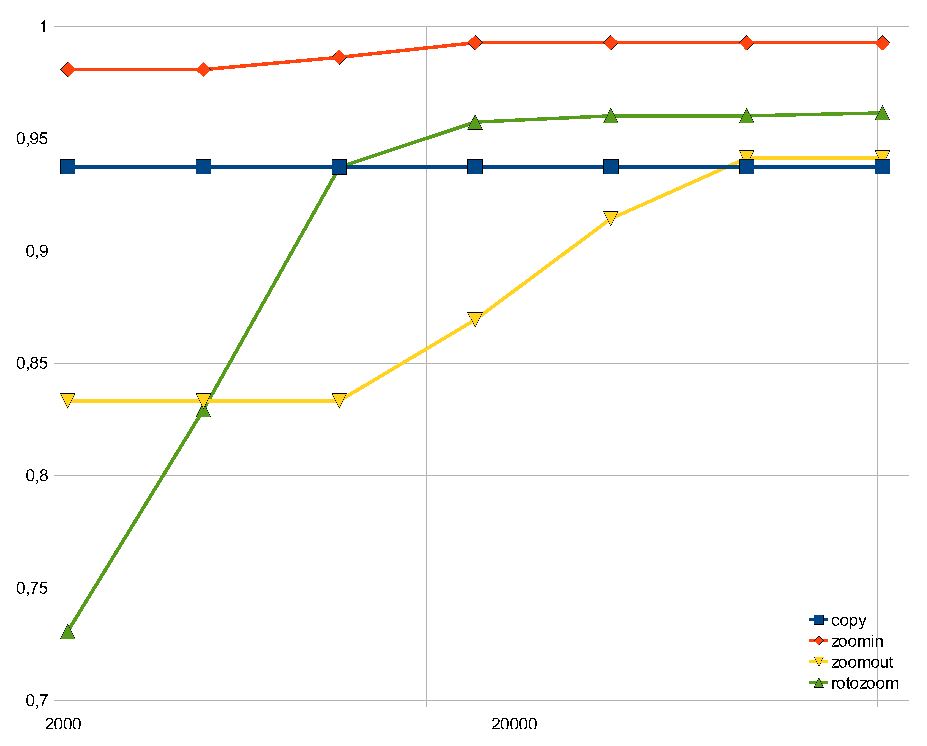
\includegraphics[height=95mm]{tcresultsgraph.eps}
\caption{Hit rates versus texel cache size. The X axis (cache size) uses a logarithmic scale.}
\label{fig:tcresultsgraph}
\end{figure}

Before we go on choosing a texel cache size, a few comments on these results can be made.
TODO

\subsection{Bilinear filter}
The bilinear filter is a straightforward arithmetic circuit that implements equation~\ref{eq:bfilter} with five pipeline sub-stages.

\subsection{Write buffer}
The write buffer is in charge of gathering the final pixels produced by the algorithm, assemble them into FML bursts and write them to the memory.

The write buffer has enough memory capacity to store two bursts on-chip. This storage space is used for a ``double buffering'' technique: while the first burst buffer receives pixels from the pipeline, the other buffer can transmit data to the memory controller. Bursts can be complete, which means that all data in them is valid, or incomplete, which means that the write buffer has not received a value for all the pixels within the burst but still needs to move the partial burst data it has off-chip because it does not have space to store it. Incomplete bursts are performed using the data mask (DM) signals of FML that will prevent some bytes from being written to the memory during the burst. Incomplete bursts should be avoided as they waste memory bandwidth and reduce performance.

This small amount of on-chip memory is enough to perform well. Indeed, the algorithm scans the rectangles one by one horizontally and then vertically (figure~\ref{fig:rectinter}) and consecutive pixels on the same horizontal line are contiguous in memory (equation~\ref{eq:fbadr}). Thus, if the destination framebuffer is aligned to the start of a FML burst and if the horizontal size of the rectangles is a multiple of the number of pixels in a FML burst, the burst buffers will be used very efficiently, with complete bursts only. This is the recommended mode of operation for the texture mapping unit.

Under this assumption, what limits the throughput of the write buffer is the time it takes to empty the second burst buffer into the memory. This time is equal to the memory write access time plus the length of the FML burst.

In the equations that follow, these symbols are used:
\begin{itemize}
\item $f$ is the system clock frequency in Hz.
\item $w$ is the width of a FML word in bits.
\item $n$ is the FML burst length.
\item $\Delta_{w}$ is the memory write access time.
\item $d$ is the number of bits per pixel.
\item $T$ is the throughput of the write buffer, in pixels per second.
\end{itemize}

We therefore have:
\begin{equation}
T = \frac{f \cdot n \cdot w}{d \cdot (\Delta_{w} + n)}
\end{equation}

Thus, the write buffer can achieve a throughput of one pixel per clock cycle ($T = f$) if the memory write access time verifies:
\begin{equation}
\Delta_{w} \leq \frac{n \cdot w}{d} - n
\end{equation}

In Milkymist, the color format uses 16 bits per pixel and the FML bus is based on bursts of four 64-bit words. Therefore, the write buffer can tolerate write latencies of up to 12 cycles while maintaining excellent performance, which seems perfectly achievable even when taking into account the delays due to bus arbitration.

\subsection{Control interface}
\label{subsec:tmucsr}
The texture mapping unit is completely under software control thanks to a CSR interface through which the CPU can configure and control it using a set of configuration and status registers. The texture mapping unit has one interrupt line to signal completion of the process to the CPU.

\section{Extra features}
Beyond this basic principle of operation, the texture mapping unit supports several features which are implemented as additional pipeline stages (not shown in figure~\ref{fig:tmublock}):
\begin{itemize}
\item Fade to black. To implement the ``decay'' effect of MilkDrop, the output picture can be darkened by multiplying all its color components by a 6-bit fixed point number between 0 and 1.
\item Chroma key. Texels of a given color can be ignored (not drawn in the output framebuffer). This is not used in normal rendering, but makes it possible to draw quickly text or symbols with transparent areas on the screen.
\item Semi-transparency (alpha blending). The output can be made semi-transparent with 64 transparency levels. This is accomplished by reading the destination picture, mixing each pixel with the output of the texture mapping (by computing a weighted average) and writing the result back to memory. If transparency is not desired, the texture mapping unit will skip reading the destination picture in order to use less memory bandwidth and avoid blocking on unneeded memory references.
\end{itemize}

\section{Implementation results}
TODO

\chapter{Floating point coprocessor}
\label{ch:pfpu}
TODO

\chapter{Software}
\label{ch:sw}
\section{LatticeMico32}
\label{sec:mico32}
The heart of the software execution capabilities of the SoC is the LatticeMico32 microprocessor core~\cite{mico32}. It is a classic 6-stage in-order pipelined RISC processor (figure~\ref{fig:lm32arch}) with a custom instruction set supported by the GNU (GCC-based) compiler toolchain. It supports separate instruction and data caches with up to two ways. There are an optional barrel shifter, pipelined multiplier and multi-cycle divider.

\begin{figure}[htp]
\centering
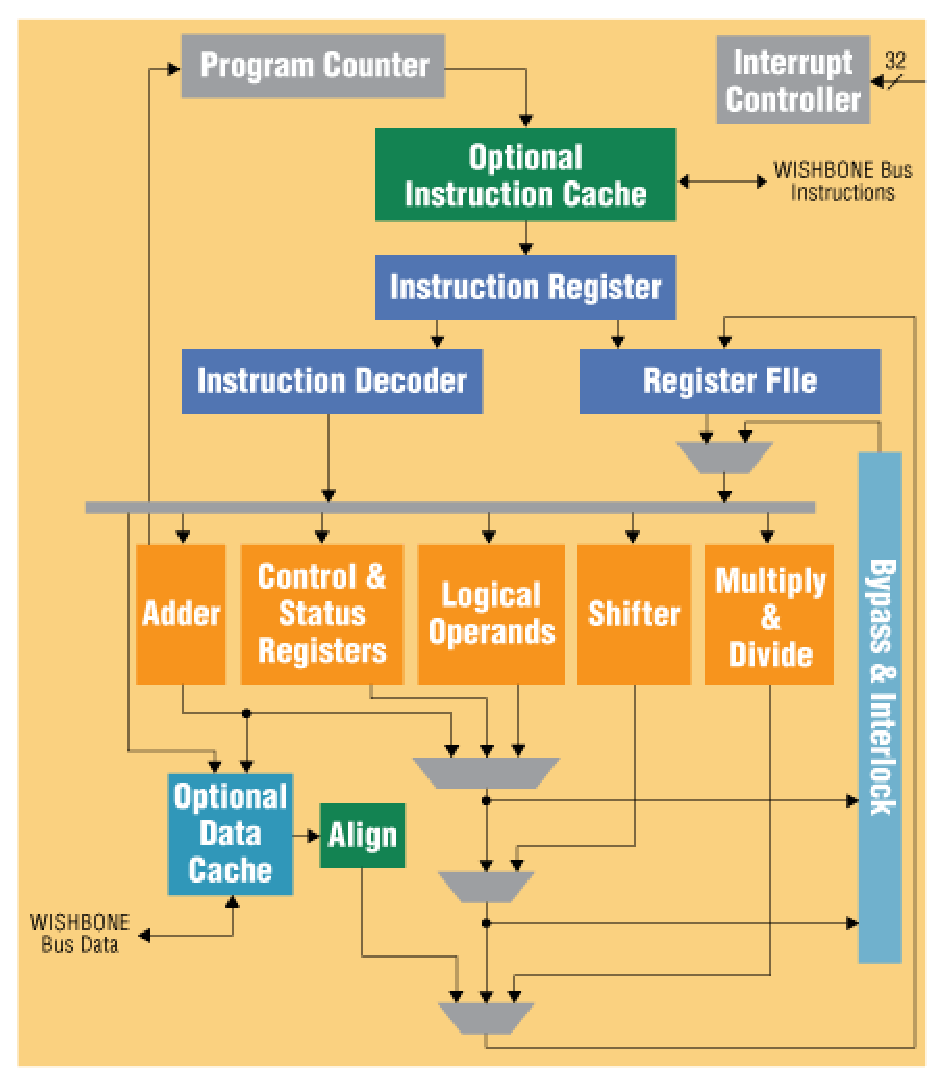
\includegraphics[height=90mm]{lm32arch.eps}
\caption{LatticeMico32 architecture (Lattice Semiconductor).}
\label{fig:lm32arch}
\end{figure}

The Milkymist system-on-chip uses LatticeMico32 with 2-way caches of 16KB each, and all the optional features enabled.

At the time this thesis is written, LatticeMico32 is the only hardware component that we have not developed specifically for the Milkymist project.

\section{Capabilities}
The ``nommu'' version of Linux has been ported to the Milkymist SoC (figure~\ref{fig:linux}). Since this is a community effort with a significant contribution by Takeshi Matsuya from Keio University, the details are not covered in this master thesis. Still, this demonstrates the ability of the platform to run complex software.

\begin{figure}[htp]
\centering
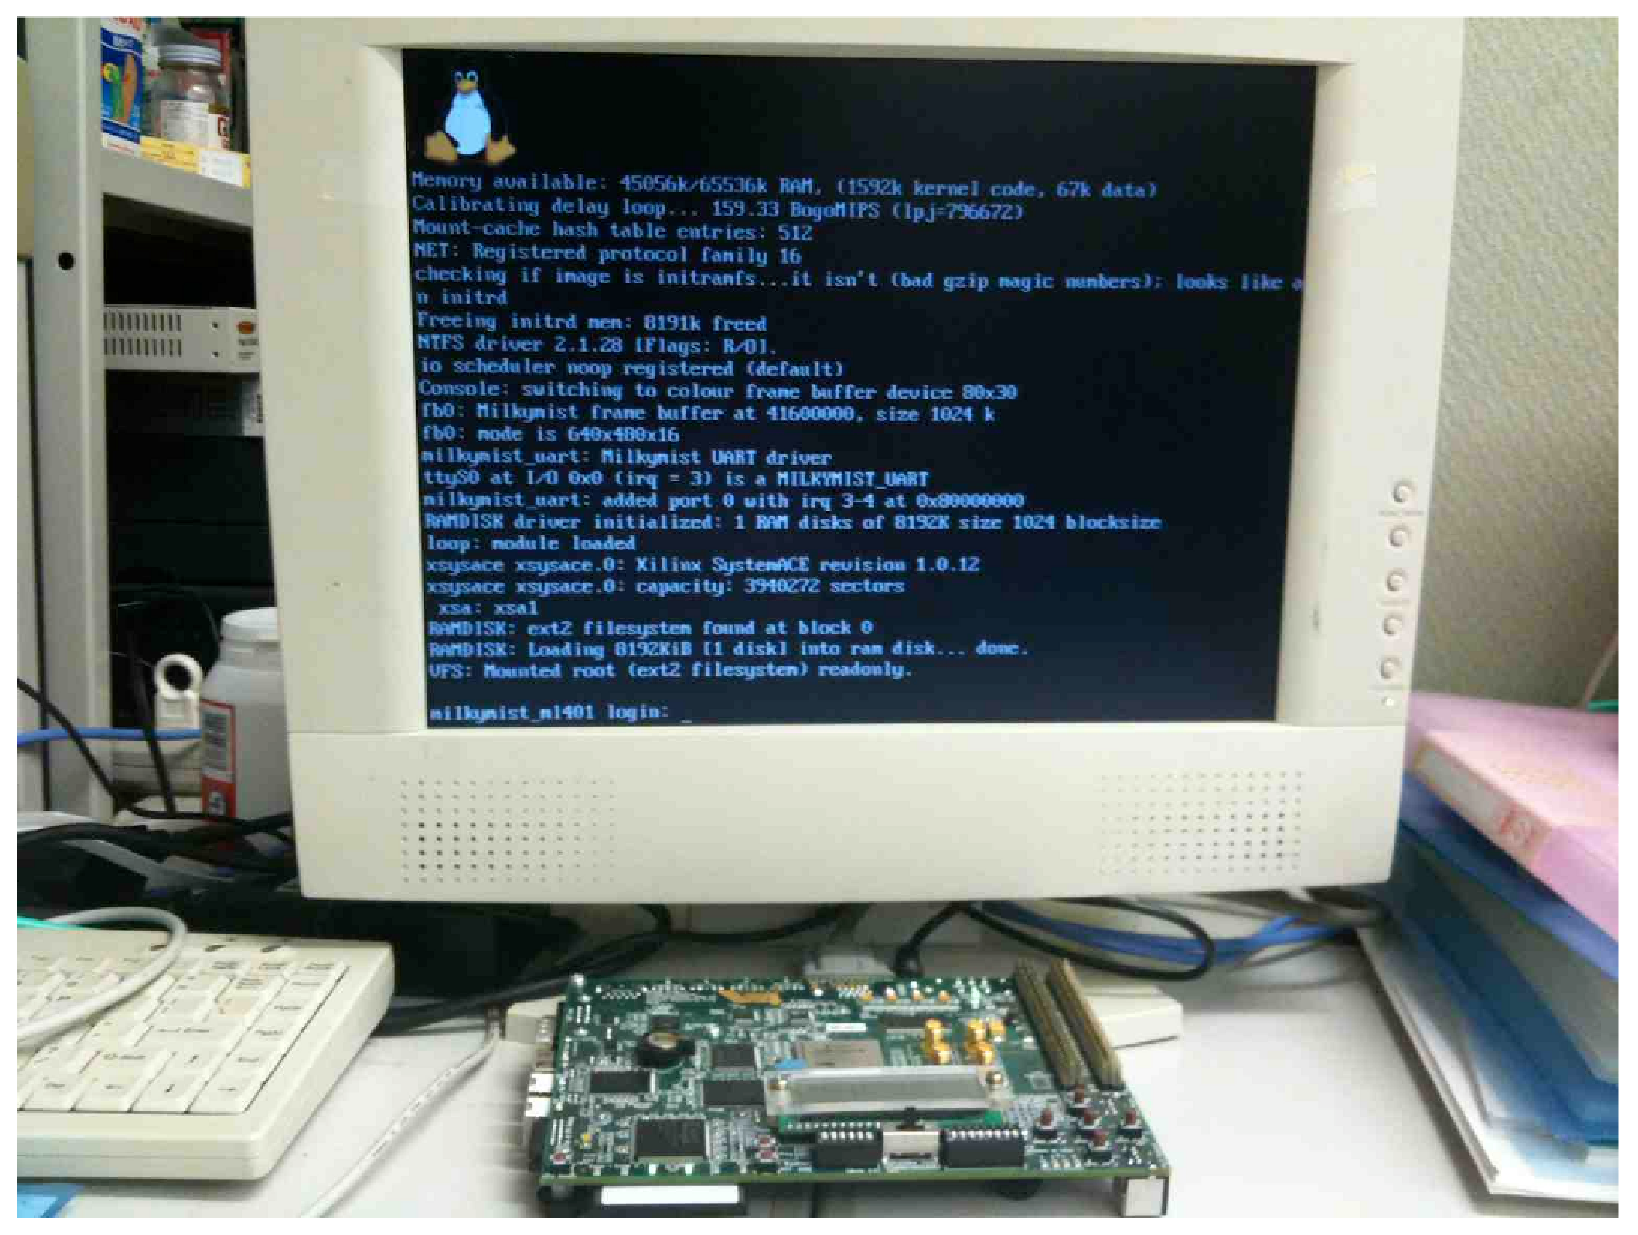
\includegraphics[height=100mm]{linux.eps}
\caption{Linux booting on the Milkymist SoC.}
\label{fig:linux}
\end{figure}

\section{Benchmarking}
The performance of the Milkymist SoC was compared to Microblaze~\cite{microblaze}, the proprietary Xilinx softcore SoC platform.

The benchmark used was the ``consumer'' MiBench~\cite{mibench} suite. By contrast to traditional benchmarks such as SPEC, MiBench is tailored to typical workloads of embedded systems. Only two benchmarks are missing from the ``consumer'' set: \verb!tiff2rgba! (it tried to use too much contiguous memory for the nommu Milkymist/Linux allocator to handle) and \verb!lame! (it crashed on Microblaze).

\begin{figure}[htp]
\centering
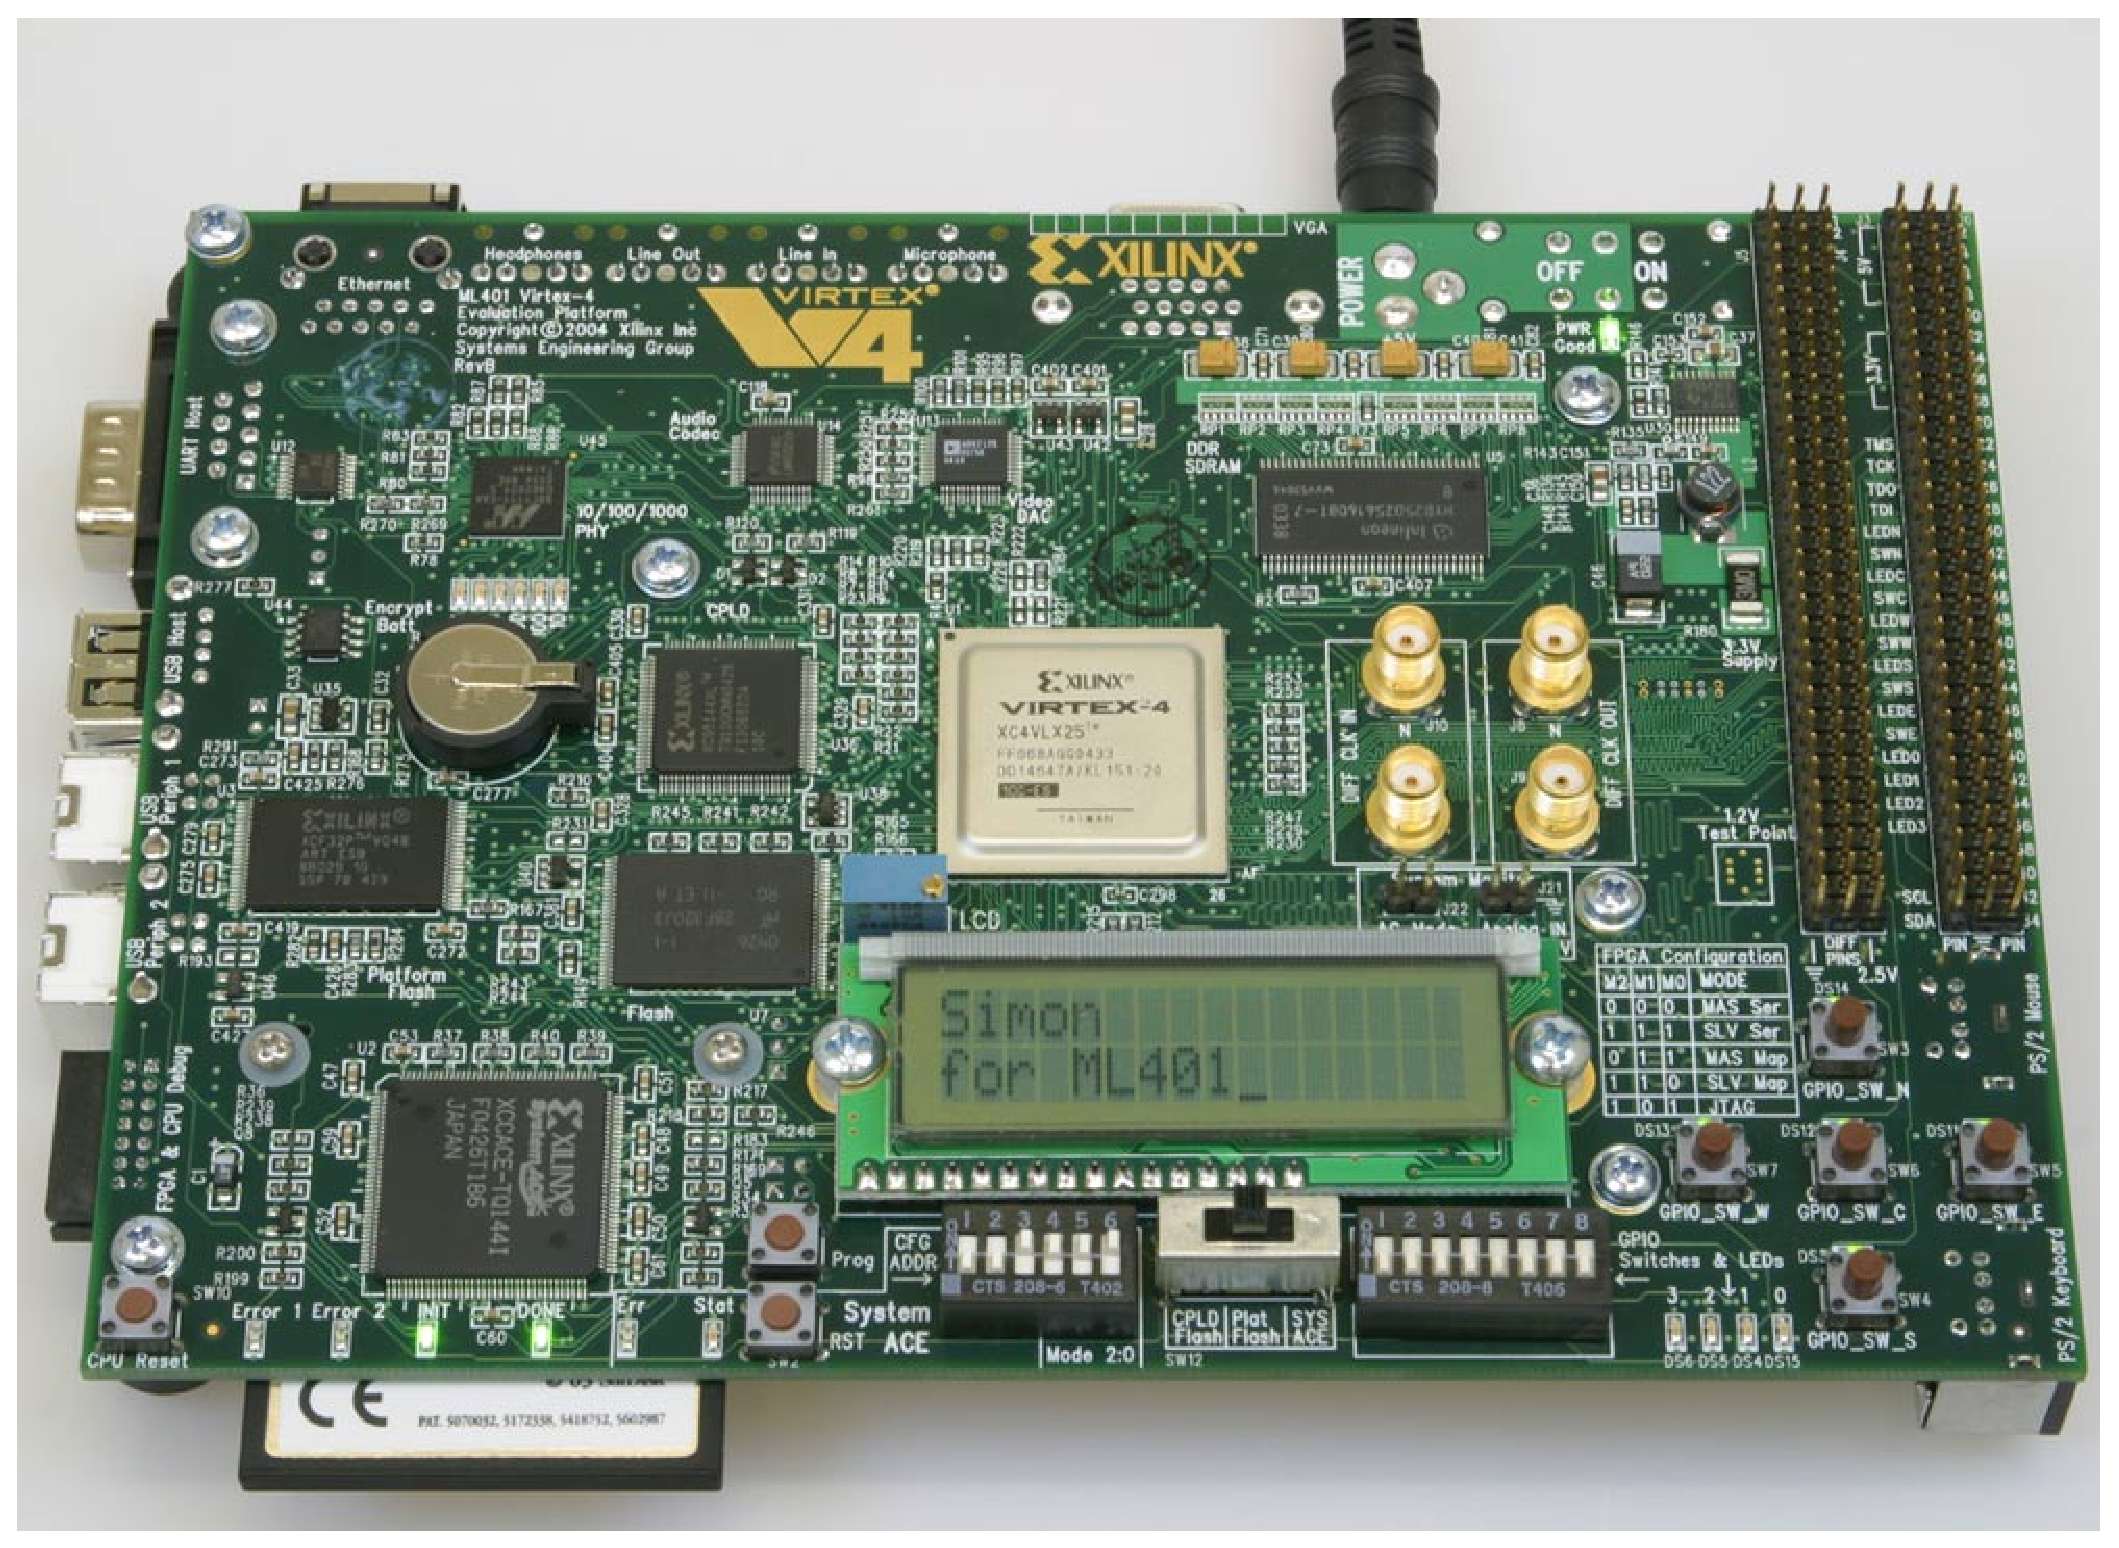
\includegraphics[height=100mm]{ml401.eps}
\caption{Xilinx ML401 development board.}
\label{fig:ml401}
\end{figure}

All tests were run on a Xilinx ML401 (XC4VLX25 FPGA, see figure~\ref{fig:ml401}) development board, with a system frequency of 100MHz.

For Milkymist, the configuration used was the default one of the port to the ML401 board:
\begin{itemize}
\item Processor with hardware multiplier, divider and barrel shifter
\item 16KB L1 instruction and data (write-through) cache (2-way set-associative)
\item No memory management unit (LatticeMico32 does not have one)
\item 16KB FML bridge write-back L2 cache (direct mapped)
\item HPDMC DDR SDRAM controller, 32-bit SDRAM bus width
\item 100MHz DDR SDRAM clock
\item Video output running at standard VGA resolution, consuming approximately 300MBps of memory bandwidth
\item Software: GCC 4.2.1 and Linux 2.6.23.
\end{itemize}

For Microblaze, the configuration is as follows:
\begin{itemize}
\item Processor with hardware multiplier, divider and barrel shifter
\item 16KB L1 instruction and data (write-through) cache (direct mapped, multi-way caches are not supported)
\item Full memory management unit
\item No L2 cache (not supported)
\item MPMC DDR SDRAM controller, 32-bit SDRAM bus width
\item 100MHz DDR SDRAM clock
\item No video output
\item Software: GCC 4.1.2 and Linux 2.6.32.4.
\end{itemize}

The comparison seems clearly in favor of Milkymist, with a rough 15\%-35\% (depending on the benchmark) reduction in execution time. Details are shown in figure~\ref{fig:mmvsmb} and in tables \ref{tab:milkymistspeed} and \ref{tab:microblazespeed}. Deviation is computed as:
\begin{equation}
\frac{|t_{1}-t_{2}|}{\textrm{min}(t_{1}, t_{2})}
\end{equation}
It is meant to check that the results are deterministic and reproducible.

\begin{figure}[htp]
\centering
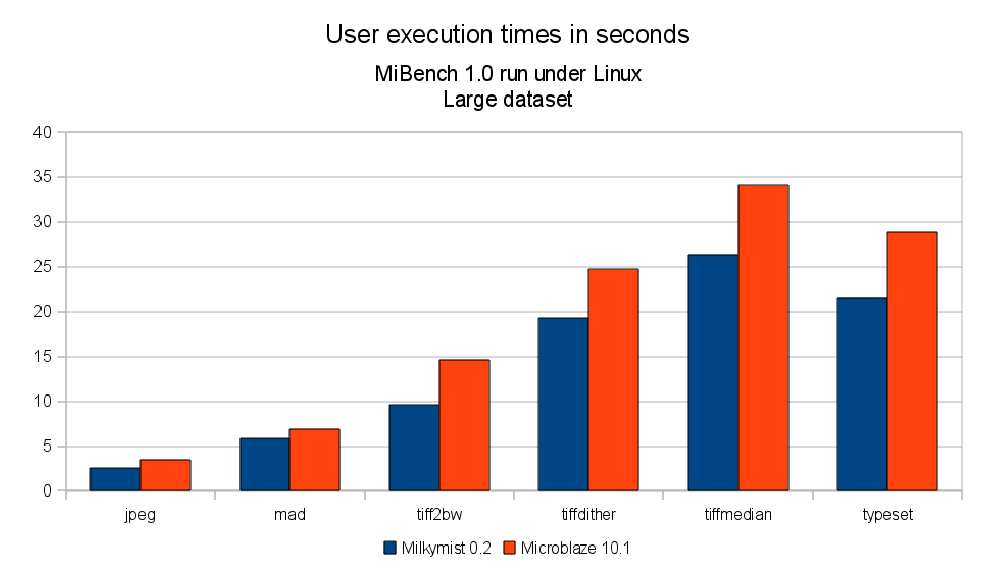
\includegraphics[height=75mm]{mm_vs_mb.eps}
\caption{Comparative MiBench results of Milkymist and Microblaze.}
\label{fig:mmvsmb}
\end{figure}

\begin{table}
\centering
\begin{tabular}{|l|l|l|l|l|}
\hline
\textbf{Benchmark} & \textbf{Run 1} & \textbf{Run 2} & \textbf{Average} & \textbf{Deviation}  \\
\hline
jpeg & 2.57 s & 2.54 s & 2.56 s & 1.18 \% \\
\hline
mad & 5.84 s & 5.87 s & 5.86 s & 0.51 \% \\
\hline
tiff2bw & 9.51 s & 9.69 s & 9.6 s & 1.89 \% \\
\hline
tiffdither & 19.28 s & 19.3 s & 19.29 s & 0.10 \% \\
\hline
tiffmedian & 26.48 s & 26.26 s & 26.37 s & 0.84 \% \\
\hline
typeset & 21.44 s & 21.79 s & 21.62 s & 1.63 \% \\
\hline
\end{tabular}
\caption{User execution times on Milkymist 0.2.}\label{tab:milkymistspeed}
\end{table}

\begin{table}
\centering
\begin{tabular}{|l|l|l|l|l|}
\hline
\textbf{Benchmark} & \textbf{Run 1} & \textbf{Run 2} & \textbf{Average} & \textbf{Deviation}  \\
\hline
jpeg & 3.42 s & 3.58 s & 3.5 s & 4.68 \% \\
\hline
mad & 6.72 s & 7.11 s & 6.92 s & 5.80 \% \\
\hline
tiff2bw & 15.19 s & 14.12 s & 14.66 s & 7.58 \% \\
\hline
tiffdither & 24.72 s & 24.68 s & 24.7 s & 0.16 \% \\
\hline
tiffmedian & 35.02 s & 33.05 s & 34.04 s & 5.96 \% \\
\hline
typeset & 28.91 s & 28.83 s & 28.87 s & 0.28 \% \\
\hline
\end{tabular}
\caption{User execution times on Microblaze 10.1.}\label{tab:microblazespeed}
\end{table}

The root causes of this performance improvement were not investigated; but since LatticeMico32 and Microblaze share a very close architecture, it is suspected that these differences are vastly explained by the combination of the low-latency HPDMC controller and the improved caches.

The main point of this comparison is to confirm the viability of Milkymist as a powerful SoC platform, that can withstand the competition with proprietary solutions.

\section{Design of a MilkDrop-like rendering program}
TODO HW/SW partitioning

\chapter{Conclusion}
TODO

\bibliography{thesis}{}
\bibliographystyle{plain}

\end{document}
